\documentclass[binding=0.6cm, LaM]{sapthesis}
\usepackage{microtype}
\usepackage[english]{babel}
\usepackage[utf8]{inputenx}
\usepackage{hyperref}
\usepackage{wasysym}
\usepackage{siunitx}
\usepackage{biblatex}
\usepackage{titlesec}
\usepackage{float}
\usepackage{xcolor}
\usepackage{nameref}
\usepackage{verbatim}
\newcommand{\fpg}[1]{\textcolor{red}{#1} }
\addbibresource{sample.bib}
\hypersetup{pdftitle={My thesis},pdfauthor={Giada Caneva Santoro}}
\usepackage{amsmath, amssymb}
\title{Coherent and Coincident Analyses of LIGO-Virgo Data from the Third Observing Run}
\author{Giada Caneva Santoro}
\IDnumber{1490713}
\course{Facolt\`a di Scienze Matematiche Fisiche e Naturali}
\courseorganizer{Corso di Laurea Magistrale in Fisica}
\AcademicYear{2018/2019}
\copyyear{2020}
\advisor{Dr. Francesco Pannarale Greco}
\authoremail{giada.greenday92@gmail.com}
\DeclareUnicodeCharacter{2212}{-}
\begin{document}

\frontmatter
\maketitle
\dedication{Fortsett å gå.}


\tableofcontents

\begin{acknowledgments}
We are grateful for computational resources provided by Cardiff University, and funded by an STFC grant supporting UK Involvement in the Operation of Advanced LIGO.
\end{acknowledgments}

\mainmatter 

\chapter*{Introduction}
\addcontentsline{toc}{chapter}{Introduction}
\markboth{Introduction}{Introduction}
%
\fpg{Giri di correzione: 1.}%
	More than 100 years ago, Albert Einstein predicted the existence of gravitational waves (GWs) starting from his theory of general relativity \cite{1,2}.
	He discovered that the acceleration of masses
	can cause distortions in the curvature of spacetime that 
        spread throughout spacetime itself at the speed of light, similarly to the ripples in a pond when a stone is tossed in it.
	He derived that the amplitude of GWs would be extremely small and concluded that it would be impossible to detect them with any of the technology foreseen at his time.

	Nowadays, roughly a century later, we are able to directly detect GWs.  The most energetic GWs are generated when high speeds and compact ojects, that is, celestial bodies with a high concentration of gravitational mass per unit volume, are involved.
	Orbiting pairs of black holes (BHs) and neutron stars (NS), the densest objects in the universe,
	are therefore efficient GW emitters and are indeed present in all the GW sources detected by the LIGO-Virgo Collaboration so far.
        BHs and NSs result from the gravitational collapse of massive progenitor stars.
        BHs represent the extremes of spacetime curvature:
        they contain a singularity, have no surface, and possess an event horizon that separates the information
        from within the BH interior from the rest of the universe.
        They are extraordinary cosmic laboratories to probe gravity in the strong-field regime.
        Astrophysical BHs are entirely described by two parameters: their gravitaitonal mass and their rotational angular momentum (spin).
        On the other hand, NSs are extreme objects from the point of view of all fundamental forces, as their masses fall in the range $1$--$2.5M_\odot$, while their radii are of the order of 10\,km; additionally, they are equipped with magnetic fields that can exceed $10^{15}\,$G (in this case one refers to the NS as magnetar). One of the main difficulties in modelling NSs is that the equation of state that governs the microphysics in their interiors is currently unknown.

        Binaries of NSs and BHs are collectively called compact binaries,
        and come in three flavours: systems that consist of two NSs (indicated as BNSs, for binary NSs), of two BHs (indicated as BBHs, for binary BHs), or of a BH and an NS (indicated as NSBHs).
        As the two compact ojects orbit one another, the binary loses orbital energy and orbital angular momentum, as both are radiated away via GWs.
        As a results, the two compact objects spiral in towards each other, 
	reaching extreme velocities ($\sim 0.5c$) at the very end of this process. 
        At the end of the inspiral, the two compact companions merge and 
	the GW emission reaches its peak. The newly formed remnant then settles down emitting a weak GW signal that dies out.  This whole process goes under the name of compact binary coalescence (CBC).
	In the final fraction of a CBC, a significant amount of gravitational mass is converted into gravitational energy carried away by the GWs.  These waves fall within the frequency range of current terrestrial GW detector, if the binary contains NSs and/or BHs with masses up to $\mathcal{O}(100M_\odot)$.
        The masses of the objects involved dictate the how long the GW signal they emit lasts in the $\sim 10$--$1000$\,Hz sensitivity band of current detectors.
        More massive binaries merge at lower frequencies and therefore have fewer cycles in band.
        For example, the first GW signal ever detected, GW150914, come from the coalescence of two fairly massive BHs: the signal was visible for only two-tenths of a second \cite{14}. 
        BNS systems, by contrast, accumulate many cycles in the instrumental band.
        The first BNS coalescence witnessed by LIGO-Virgo, GW170817, generated a GW signal that lasted $\sim 100\,$s in the sensitivity window of the detectors \cite{15}.
	The observation of GW150914 was a truly remarkable accomplishment: it \emph{directly}\footnote{Until then, GWs had only been observed indirectly by using pulsars timing to monitor 
        their effect on the orbit of pulsar binary star systems.} confirmed Einstein's prediction of the existence of GWs, and it demonstrated that stellar-mass BBH systems form in the universe and merge within a Hubble time.
	This event marked the beginning of a new era of GW astronomy, 
	which enables the observations of violent astrophysical events that are not visible with traditional astronomy.
	The BNS merger GW170817 marked, instead, the beginning of multi-messenger astronomy 
	because as it was the first GW observation with recorded electromagnetic counterparts.  \fpg{Per antrambi questi eventi, aggiungi una forward reference alle sezioni in cui le discuti.}

	The LIGO-Virgo GW network routinely performs multiples searches aimed at detecting signals emitted by all three kinds of CBCs\footnote{See Sec.\,\ref{sec:sources} for a brief overview of other kinds of seraches.}.
        These are run both online, to detect and report compact binary merger events 
	with sub-minute latencies, and offline, to take advantage of improved data calibration 	
	and of additional information regarding data quality to produce a more sensitive search.
	This thesis focuses on two kinds of offline analyses of a part of LIGO-Virgo data collected during the third observing run (O3).
        Specficially, I used the CBC matched-filtering search pipeline {\ttfamily PyCBC}, discussed in Chapter \ref{ch:datatools}, to perform an all-sky search for BNS, NSBH, and BBH signals; further, I used the {\ttfamily PyGRB} pipeline, discussed in Chapter \fpg{...}, to search for BNS and NSBH signals compatible with the sky-location and time of three short gamma-ray bursts (GRBs) that occured during O3.

        \fpg{Tutta la parte sui GRB richiede delle citazioni.}
	GRBs are short ($\Delta t \sim 0.1-100s$) and intense bursts of 
	electromagnetic radiation in the high-energy (1\,keV--10\,MeV) $\gamma$-ray spectrum.
	This radiation is produced when an ultra-relativistic fireball of high energy photons 
	is launched from a central engine, and it can be accompanied by a detectable afterglow emission 
	in the X-ray and sometimes optical and radio bands, as the fireball expands and cools down.
	GRBs can be broadly classified based on the timescale during which 5\% to 95\% of the counts are recorded ($T_{90}$)
	as either long GRBs, $T_{90} > 2\,$s or short GRBs, $T_{90} \geq 2\,$s.
	The two groups also show other differences.  Short GRBs have fainter afterglows and harder emission spectra than long GRBs; they are also seen to have an offset relative to their host galaxy center.
	For decades, the exact origin of short GRBs was an open question in high-energy astrophysics.  The data indicated a compact source smaller than a stellar-scale object, and a progenitor involving old astrophysical objects with a significant velocity with respect to the host galaxy.  BNS and NSBH mergers were the natural candidates as short GRB progenitors, but the observational confirmation of this conjecture came with GW170817.
	This event marked the first direct observation of a BNS unambiguously associate to a short GRB, GRB 170817 which followed $1.74\,$s after the GW trigger and was detected by {\it Fermi}/GBM and INTEGRAL SPI-ACS.
	The unambiguous association also allowed for the most precise comparison to date
	between the speed of GWs and the speed of light.  Further, it posed new constraints on alternative theories of gravity. 
	Subsequent electromagnetic follow-up of GW170817 showed that BNS merger events 
	help explain the origin of heavy elements in the universe.

	There remain several open questions surrounding these extreme and energetic events, 
	and multi-messenger astronomy with GWs has proven to be a resourceful means of gaining 
	knowledge of the astrophysical sources and their emission engines, 
	providing insight that electromagnetic observations alone cannot achieve.
	To mention a few examples of open problems, we do not yet know whether NSBH systems are also short GRB progenitors.  Similarly, the exact mechanism that launches the jet is currently not yet understood.
        These and other questions motivate the targeted searches for GWs at the sky-position and time of GRBs, as they increase the chances of achieving joint GW-GRB detections.
	Knowing the time and sky-location of a sought for GW event
	allows to perform a deeper search in the GW data, potentially uncovering signals that are not accessible to all-sky, all-time searches \fpg{forward reference.}

	Since the observed properties of short GRBs may be attributed to matter accretion onto a BH,
	following the tidal disruption of a NS, in addition to BNSs, NSBH systems are also considered likely short GRBs progenitors.
	At the time of writing this work, no certain NSBH coalescence has been observed.
	This motivates further the use of 
	offline GW searches targetting short GRB triggers, as the one I conducted in Chapter $\ref{ch:datanalysis}$.
	To enable this search in O3, I also generated and validate the set of waveforms used to filter the data (see discussion in Sec\,\fpg{...})
	This specific set of waveform is known as an ``EM-bright template bank,'' 
	as it covers only BNSs and NSBH sytems that have undergone tidal disruption and are thus potential short GRB progenitors.

	This thesis is organized as follows: Chapter \ref{ch:GWDetectionPrinciples} provides a theoretical introduction to gravitational waves and 
	describes the LIGO and Virgo detectors and the physics behind its purpose, and noise sources.
	Chapter \ref{ch:datatools} gives an introduction to data analysis tools for a matched filtering source, 
	describes the generation of template banks and signal consistency tests.
	It then provides an overview of coherent vs coincident searches; the last section describes injections.
	Chapter \ref{ch:ObservingRuns} gives a summary of the gravitational wave detection from the first to the third observing run.
	Chapter \ref{ch:datanalysis} illustrates the difference between the old and new model for the remnant mass of a neutron star-black hole system.
	It then describes how the template bank has been updated and how well it works.
	Finally, the results of the offline {\ttfamily PyCBC} and {\ttfamily PyGRB} search are presented and discussed.

%----------------------------------------------------------------------------------------------------------------------------------------------------------------------------------------------------------
\chapter{Gravitational-Wave Detection Principles}
\label{ch:GWDetectionPrinciples}
\fpg{Giri di correzione: 1.}%
	The aim of this thesis is to expose the methodologies involved 
	in compact binary coalescence through gravitational wave observation. 
	Before giving into this topic, it is useful to shortly discuss gravitational waves, 
	the theory behind them and the instrumental apparatus that is being used to detect them. 
	In this chapter we give a broad outline of these subjects, 
	without going too deep into details. \\
	We begin by introducing the basics of gravitational wave theory in section 2.1. 
	In section 2.2 we discuss gravitational wave interferometric detectors. 
	In section 2.3 we briefly describe the noise sources that affect the detection. 
	Finally. in section 2.4, we describe the astrophysical sources of gravitational radiation.

\section{Gravitational waves in linearized gravity}

	In 1915, Albert Einstein presented his general theory of relativity
	The classical Newtonian notion of gravity, which stated that gravity arises from an 
	action at a distance, was replaced by a geometric interpretation of the Universe, 
	the spacetime continuum: this may be regarded as a fabric and that can be curved 
	by mass \cite{1}. 
	The motion of masses on this curved spacetime fabric will then be perceived as gravity. 
	In general relativity, spacetime is regarded as a four-dimensional manifold 
	with a Lorentzian metric, and gravity is a manifestation of the manifold’s curvature. \\
	The space-time curvature is associated with the stress-energy tensor 
	of matter fields through the Einstein field equation:
		\begin{equation}
		G_{\mu\nu} \equiv R_{\mu\nu}  - {1 \over 2}g_{\mu\nu}R = {8\pi G_{N} \over {c^4}}T_{\mu\nu} 
		\end{equation}
	where $G_{\mu\nu} $ is the Einstein tensor, $T_{\mu\nu} $ is the stress-energy 
	tensor of matter-fields, $ G_{N}$ is Newton’s gravitational constant and $c$ the speed of light. \\
	In 1916 Einstein found the weak-field solutions to general relativity had wave-like solutions, GWs.
	GWs are ripples in the fabric of spacetime, 
	which periodically lengthen and shorten space, and speed up and slow down time \cite{2}.
 	To study the properties of GWs, it is instructive to first study them 
	in situations where the gravitational fields are weak.
	In the so-called weak-field approximation, one can view the metric as the Minkowski metric 
	with a small perturbation: the Einstein equations can be expanded around the flat-space metric, of special relativity. \\
	Letting $ x_\mu = (t, x, y, z)$ denote the time and space coordinates, 
	we can write the proper distance between events $x_{\mu}$ and $x_{\mu} + dx_{\mu}$ as
		\[
		ds^2 = g_{\mu\nu}dx^{\mu}dx^{\nu} \approx (\eta_{\mu\nu} + h_{\mu\nu})dx_{\mu}dx_{\nu}. \hspace*{2cm}\|h_{\mu\nu}\|\ll 1
		\]
	Here $\eta_{\mu\nu} = diag(-1,1,1,1)$ is the usual Minkowski metric and the metric perturbation  $h_{\mu\nu}$        
	represents the linearised gravitational field, it encapsulates GWs, 
	but contains additional, non-radiative degrees of freedom as well. $\|h_{\mu\nu}\|$ means
	“the magnitude of a typical non-zero component of $h_{\mu\nu}$”. 
	The condition $\|h_{\mu\nu}\|\ll 1$ requires both the gravitational field to be weak, 
	and constrains the coordinate system to be approximately Cartesian.  \\
	In linearized gravity, the smallness of the perturbation means that only terms which are linear in $h_{\mu\nu}$ are considered;
	higher order terms are discarded. As a consequence, indices are raised and lowered using the flat metric. 
	The metric perturbation $h_{\mu\nu}$ transforms as a tensor under Lorentz transformations, 
	but not under general coordinate transformations: since the numerical values of the components
	of a tensor depend on the reference frame, there exists a reference frame in which 
	the linearisation of the gravitational field holds on a sufficiently large region of the spacetime. \\
	The Einstein field equations are covariant under general coordinate transformations
		\begin{equation}
		x^{\mu} \rightarrow x^{\mu ‘}(x)
		\end{equation}
	So that the metric transforms as
		\begin{equation}
		g_{\mu\nu} \rightarrow g_{\mu' \nu'} = x^{\rho},_{\mu'}x^{\sigma},_{\nu'}g_{\rho \sigma}
		\end{equation}
	This means that one is free to choose a convenient coordinate system without 
	altering the physical predictions of the field equations \cite{16}. \\
	Choosing a reference frame breaks the invariance of general relativity under 
	coordiante trasformations but it also erases spurious degrees of freedom. 
	After choosing a frame where the field is linearised, 
	a residual gauge symmetry remains. \\
	Under infinitesimal coordinate transformations
                 \[
			x_{\mu} \rightarrow x_{\mu} + \xi_{\mu}
                \]
	using the transformation law of the metric, to lowest order $h_{\mu\nu}$ transforms as	
		\[
			h_{\mu\nu} \rightarrow h_{\mu\nu} - \partial_{\mu}\xi_{\nu} - \partial_{\nu}\xi_{\mu}
		\]
	Rather than working with the metric perturbation, changing notation and using the trace-reversed perturbation 
	makes the computation more compact and cleaner. We define
		\begin{equation}
			{\bar h}_{\mu\nu} = h_{\mu\nu} - {1 \over {2}}\eta_{\mu\nu}h  
		\end{equation}
	the trace
		\begin{equation}
			h = \eta^{\mu\nu}h_{\mu\nu}
		\end{equation}
	and express the trace-reversed field:
		\begin{equation}
			h_{\mu\nu} = {\bar h}_{\mu\nu} + {1 \over {2}}\eta_{\mu\nu}{\bar h}
		\end{equation}
	The Rienmann tensor constructed in the linearised theory is given by
		\begin{align}
			R^{\mu}_{\nu\rho\sigma} &= \partial_{\rho} \Gamma^{\mu}_{\nu\sigma} - \partial_{\sigma}\Gamma^{\mu}_{\nu\rho}  \\
				       &= {1 \over 2} (\partial_{\rho}\partial_{\nu}h^{\mu}_{\nu\rho} + \partial_{\sigma}\partial^{\mu}h^{\nu\rho} - \partial_{\rho}\partial^{\mu}h^{\nu\sigma} - \partial_{\					     \sigma}\partial_{\nu}h^{\mu}_{\rho})
		\end{align}
	From this, the Ricci tensor takes the form
		\begin{equation}
			R_{\mu\nu} = R^{\rho}_{\mu\rho\nu} = {1 \over 2}(\partial_{\rho}\partial_{\nu}h^{\rho}_{\mu} + \partial^{\rho}\partial_{\mu}h_{\nu\rho} - \square h_{\mu\nu} - \partial_{\mu}\partial_{\nu}h)
		\end{equation}
	The curvature scalar is obtained contracting once more:
		\begin{equation}
			R = R^{\mu}_{\mu} = (\partial_{\rho}\partial^{\mu}h^{\rho}_{\mu} - \square h)
		\end{equation}
	Finally, the Einstein tensor can be expressed as
		\begin{equation}
			G_{\mu\nu} = {1 \over 2}(\partial_{\rho}\partial_{\nu}h^{\rho}_{\mu} + \partial^{\rho}\partial_{\mu}h_{\nu\rho} - \square h_{\mu\nu} - \partial_{\mu}\partial_{\nu}h - \eta_{\mu\nu}\partial_{\rho}\partial^{\sigma}h^{\rho}_{\sigma} + \eta_{\mu\nu}\square h)
		\end{equation}
	Substituting the metric perturbation $h_{\mu\nu}$  with the $trace-reversed$ perturbation ${\bar h}_{\mu\nu}$ and expanding, 
	the linerised Einstein equations take the compact form:
		\begin{equation}
			\square {\bar h}_{\mu\nu} + \eta_{\mu\nu}{\partial}^{\rho}{\partial}^{\sigma}{\bar h}_{\rho\sigma} - {\partial}^{\rho}{\partial}^{\nu}{\bar h}_{\mu\rho} - {\partial}^{\rho}{\partial}^{\mu}{\bar h}_{\nu\rho} = - {{16\pi G_{N}} \over {c^4}}T_{\mu\nu}.
		\end{equation}
	The linearised equations of motion are gauge-invariant, and the gauge freedom can
 	be used to simplify the form of the field equations \cite{17}.
 	In the Lorentz family of gauges, choosing the harmonic gauge $ \partial_{\mu}h_{\mu\nu} = 0 $ 
	reduces the Einstein equations to a simple wave equation that relates the trace-reversed field
 	to the stress energy tensor:
		\begin{equation}
			\label{reduceinstein}
			\square {\bar h}_{\mu\nu} =({\partial^2 \over {\partial t^2} } - {\partial^2 \over {\partial x^2}}  - {\partial^2 \over {\partial y^2}}  -  {\partial^2 \over {\partial z^2}}) {\bar h}_{\mu\nu} = -{{16\pi G_{N}} \over {c^4}}T_{\mu\nu}. 
		\end{equation}
	By imposing the harmonic gauge one has chosen the coordinates in such a way that for a single plane wave 
	(or a superposition of plane waves with their wave vectors pointing in the same direction),
	the GW polarisations are perpendicular to the direction of propagation.
	The harmonic gauge gives four conditions, that reduce the ten indipendent components of  
	$h_{\mu\nu}$ to six indipendent components, so it does not fix the gauge completely,
	leaving four additional components free to be gauge-fixed.
	If the metric perturbation is not in the harmonic gauge, by making an infinitesimal coordinate transformation
		\begin{equation}
			{\bar h}_{\mu\nu} \rightarrow {\bar h}_{\mu’\nu’}  = {\bar h}_{\mu\nu}  - \xi_{\mu,\nu} -\xi_{\nu,\mu} + \eta_{\mu\nu}\xi^{\rho}_{,\rho}
		\end{equation}
	and applying the harmonic gauge condition
		\begin{equation}
			{\bar h}_{\mu’\nu’,} ^{\nu’} = {\bar h}_{\mu\nu,} ^{\nu} - \xi_{\mu,\nu}^{\nu}
		\end{equation}
	Therefore any metric perturbation can be put into an harmonic gauge by making an infinitesimal 
	coordinate transformation that satisfies
		\begin{equation}
			{\bar h}_{\mu\nu,} ^{\nu} = \xi_{\mu,\nu}^{\nu}
		\end{equation}
	This is a wave equation that always admits a solution, thus one can always achieve the harmonic gauge. 
	Outside the source where $T_{\mu\nu} = 0$ Eq.$\ref{reduceinstein}$ reads 
		\begin{equation}
			\square {\bar h}_{\mu\nu} = 0
		\end{equation}
	In asymptotically flat ($h_{\mu\nu} \rightarrow 0$ as $r \rightarrow 0$) vacuum spacetimes, 
	the metric perturbation can be greatly simplified using
	the residual gauge freedom within the harmonic gauge class \cite{4}. 
	The transverse-traceless $TT$-gauge can be obtained by choosing the components of the metric tensor $h_{\mu\nu}$
	so that only the ones on the plane orthogonal to the direction of propagation (transverse) 
	are different from zero; this results in $h_{\mu\nu}$ being traceless:
		\begin{equation}
			h^{0\mu} = 0 \hspace*{0.5cm}  h^{i}_i = 0  \hspace*{0.5cm}   {\partial}^jh_{ij} = 0
		\end{equation}
	By imposing the harmonic gauge, the ten degrees of freedom of $h_{\mu\nu}$ 
	have reduced to six degrees of freedom, and the residual gauge freedom,
	associated to the four functions $\xi^{\mu}$, has further reduced these to just two degrees of freedom, 
	which correspond to the two possible polarization states of the GW. 
	Equation (2.17) has plane wave solutions $h_{\mu\nu}^{TT}(x)=e_{ij}(k)e^{ikx}$ with 
	$k^{\mu}=(\omega/c,k)$ and $\omega/c=|k|$. The tensor $e_{ij}(k)$ is called the polarization tensor. \\
	In vacuum spacetimes, a plane GW with a given wave-vector $k$ is characterized 
	by two functions $h_+$ and $h_{\times}$, while the remaining components can be set to zero by
	choosing the transverse-traceless gauge. 
	Along the z axis:
		\begin{equation} 
		h_{\mu\nu}^{TT} = 
		\begin{bmatrix}
		0 & 0 & 0 & 0 \\
		0 & h_{+} & h_{\times} & 0 \\
		0 & h_{\times} & -h_{+} & 0 \\
		0 & 0 & 0 & 0 
		\end{bmatrix}\cos{\omega(t-z/c)}
		\end{equation}

\subsubsection{Geodesic equation and geodesic deviation}

	The usual notion of “gravitational force” disappears in general relativity, replaced instead 
	by the idea that freely falling bodies follow geodesics in spacetime.
	Geodesics are the curved-spacetime equivalents of straight lines, which can be found by 
	parallel transporting the tangent vector of a curve \cite{16}. \\
	Given a spacetime metric $g_{\mu\nu}$ and a set of spacetime coordinates $x^{\mu}$, 
	geodesic trajectories are given by the equation:
		\begin{equation}
			{{d^2x^{\mu}}\over{d\tau^2}} + \Gamma_{\nu\rho}^{\mu}(x){{dx^{\nu}}\over{d\tau}}{{dx^{\rho}}\over{d\tau}} = 0 \hspace*{2cm} m \neq 0
		\end{equation}
		\begin{equation}
			{{d^2x^{\mu}}\over{d\lambda^2}} + \Gamma_{\nu\rho}^{\mu}(x){{dx^{\nu}}\over{d\lambda}}{{dx^{\rho}}\over{d\lambda}} = 0 \hspace*{2cm} m = 0
		\end{equation}
	which is the classical equation of motion of a test mass in the curved background described 
	by the metric $g_{\mu\nu}$, in the absence of an external non-gravitational force and where $m$ is the mass
	of the object, $\tau$ represents the proper time given by $d\tau^2 = -ds^2$, 
	and $\lambda$ is some affine parameter along the geodesic. \\
	In a flat spacetime, two straight lines that are initially parallel to each other will remain parallel. \\
	In a curved spacetime, geodesics do not satisfy this property.
	Instead, two nearby geodesics, separeted by $\zeta^{\mu}$, follow the geodesic deviation equation
		\begin{equation}
			{{D^2\zeta^{\mu}}\over{D\tau^2}} = -R^{\mu}_{\nu\rho\sigma}\zeta^{\rho}{{dx^{\nu}}\over{d\tau}}{{dx^{\sigma}}\over{d\tau}}
		\end{equation}
	where $D/D\tau$ is defined as
		\begin{equation}
			{{DV^{\mu}}\over{D\tau}} \equiv {{dV^{\mu}}\over{d\tau}} + \Gamma^{\mu}_{\nu\rho}V^{\nu}{{dx^{\rho}}\over{d\tau}}
		\end{equation}
	and denotes the covariant derivative along a curve parameterised by $\tau$. 
	The geodesics deviation equation describes the change in separation $\zeta^{\mu}$ between two nearby geodesic. \\
	As the Rienmann tensor describes the tidal forces caused by the gravitational field, 
	the geodesic deviation equation shows that tidal forces can be considered as deviations of nearby geodesics \cite{6}.

%----------------------------------------------------------------------------------------------------------------------------------------------------------------------------------------------------------
\section{Gravitational-wave detection with laser interferometers}

	Electromagnetic waves interact strongly with matter, while GWs travel unperturbed through space,
        as they interact only very weakly with matter. This makes them an excellent probe for astrophysical phenomena that are dark
        in the electromagnetic channel, such as the coalescence and merger of BHs, the collapse of a stellar core,
  	the dynamics of the early Universe. \\
	However, it also means that detecting GWs is extremely challenging.
        Electromagnetic radiation typically has a wavelength smaller than the size of the emitting system,
        and so can be used to form an image of the source, while the wavelength of gravitational radiation is typically comparable
        to or larger than the size of the radiating source \cite{18}. 
        Because GWs are generated by the bulk dynamics of the source itself therefore they cannot be used to form an image:
        the radiation simply does not resolve the generating system.
        In most cases, electromagnetic astronomy is based on observers obtain a large amount of information about sources on a small piece
        of the sky while GW astronomy is intrinsically an all-sky approach \cite{4}. \\
	The experimental search for GWs was initiated by Joseph Weber in the early 60  \cite{7}.
	Weber’s first GW detector was a resonant bar detector; 
	the detection’s principle behind these instruments is that 
	they would be set into oscillation at their resonant frequency 
	by passing GWs near that resonant frequency.
	For this purpose, Weber designed and built a big aluminum cylinder as a sort of antenna, 
	hung by a steel wire from a support to isolate vibrations of its environment. 
	The whole instrument was placed inside a vacuum chamber 
	and the cylinder surrounded by a belt of piezoelectric crystal, 
	to sense cylinder vibrations induced by GWs.
	Even though, over the course of the following years, the bar detectors’ sensitivity increased, 
	it did not reach a level where they would be able to detect an extragalactic source. \\
	The first explicit suggestion of a laser interferometer detector 
	was outlined by Gertsenshtein and Pustovoid in 1962 \cite{8}. \\
	From the early 2000s, several kilometer-scale ground-based interferometers 
	operated in the frequency band from 10 Hz to 1 kHz at a sensitivity 
	that all owed the potential for detection from a variety 
	of sources at large extragalactic distances.

\subsection{Description of laser interferometers}

	The optical layout of the detectors consists in perpendicular 
	Fabry–Perot arm cavities of the Michelson, 
	with lasers running along the 4 km arms, as shown in Fig.$\ref{fig:interferometer}$. 
	A beam splitter directs 1064 nm light from a diode-pumped, power amplified, 
	and intensity and frequency stabilized Nd:YAG laser to the Fabry-Perot arms, 
	which are made of an input test mass mirror and an end test mass mirror. 
	The two beams of laser light that return from the two arms are recombined out of phase so that, 
	in principle, no light reaches the so-called 'dark fringe' of the detector. 
	The oscillating quadrupolar strain pattern of a GW, 
	as seen in Fig.$\ref{fig:ring}$, is well matched by a Michelson interferometer,
        which makes a very sensitive comparison of the lengths of its two orthogonal arms.
	Any variation caused by an alteration in the distance between the mirrors, 
	produces a very small shift in phase between the beams and, thus, 
	a variation of the intensity of the light, which is proportional to the wave's amplitude. \cite{10}. \\
	The Fabry-Perot arms are a modification to the Michelson 
	that increases the change in phase measured compared to that for a simple Michelson: 
	because of multiple reflections that occur within each cavity, 
	the tiny distance variation caused by a GW is amplified. 
	All the main interferometer optical components and beam paths are enclosed in the ultra-high vacuum system
        $(10^{−8} - 10^{−9} torr)$ for acoustical isolation and to reduce phase fluctuations from light scattering off residual gas.
        The photodetectors are all located outside the vacuum system, mounted on optical tables.
        The beam tubes are made from stainless steel and are designed to have low-outgassing
        so that the required vacuum can be attained by pumping only from the ends of the tubes \cite{11}. 
        The interferometer optics, including the test masses, are manufactured to have extremely low scatter and low absorption. \\
	The GW detectors offer the possibility of very high sensitivities over a wide range of frequency and
        are particularly suited for the detection of local perturbations in the spacetime metric from astrophysical sources,
        such as binary BH (BBH), or NS coalescences, asymmetric rapidly spinning NSs,
        and supernovae.
 	Gravitational radiation is produced by oscillating multipole moments of the mass distribution of a system.
        Quadrupole radiation is the lowest allowed form, and is thus usually the dominant form.
        In this case, the GW field strength is proportional to the second time derivative of the quadrupole moment of the source,
        and it falls off in amplitude $h$, the direct observable of gravitational radiation, with distance as $1/r$.
        This comparatively slow fall off with distances means that relatively small improvements in the sensitivity
        of GW detectors can have a large impact on their science:
        doubling the sensitivity of a detector doubles the distance to which sources can be detected,
        increasing the volume of the Universe to which sources are measurable by a factor eight. \\
	The frequency band $1Hz \apprle f \apprle 10^4 Hz$ is targeted by
        ground-based laser interferometric detectors has its low end set by the fact that it is extremely difficult
        to prevent mechanical coupling of the detector to ground vibrations at low frequencies,
        and probably impossible to prevent gravitational coupling to ground vibrations, human activity, and atmospheric motions.
    \begin{figure}[H]
                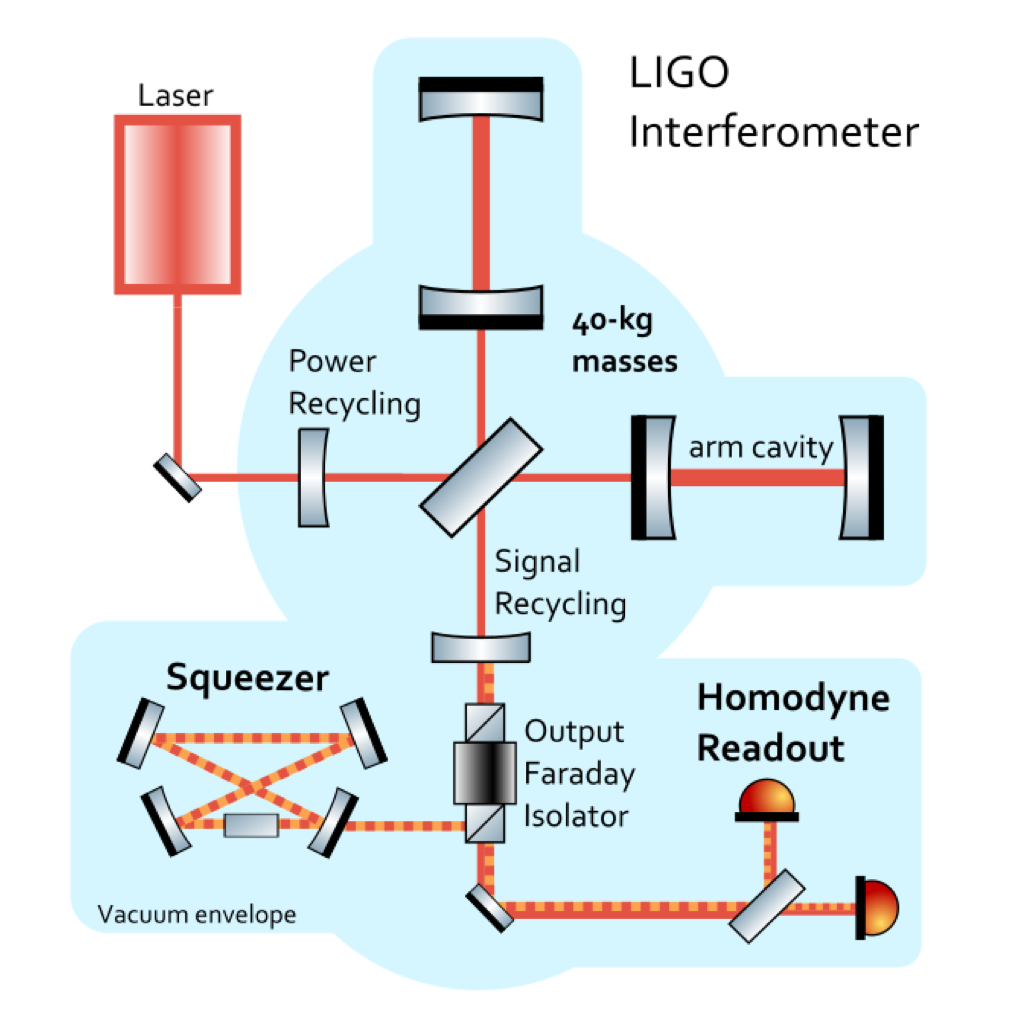
\includegraphics[scale=0.5]{interferometer}
                \centering
                \caption{Simplified schematic of the experimental setup. Several modifications to the Michelson interferometer are shown such as power and signal recycling. The photodetector records the differential lengths of the arms. \cite{9}}
                \label{fig:interferometer}
                \end{figure}

\subsection{Ground-based laser interferometers}

	Detectors have nearly $4\pi$ steradian sensitivity to events over the sky. 
	This means that any source on the sky will be detectable,
        not just sources in specific pointing directions. \\
	A single interferometer is unable to detect GW alone,
	because it us difficult to separate a signal from noise confidently 
	and also provides no directional information about the source.
	A worldwide network of detector is essential to a successful GW detection:
	looking for identical, simultaneous signals from multiple detectors worldwide, 
	rules out noise sources which are local to a given detector. 
	More detectors means a better determination of the direction of GW sources: 
	to reconstruct the location of a transient signal is primarily due to triangulation 
	based on the observed time delays of the signal at several detectors. 
	For more than two sites, requiring a consistency between the observed amplitudes 
	will also serve to restrict the allowed sky positions\cite{12}. \\
	A crucial aspect of the research is to make the instrument sufficiently sensitive:
        at the targeted strain sensitivity of $10^{−21}$ m, the resulting arm length change is only $ 10^{-18}$ m for km-scale instruments, that is
        a thousand times smaller than the diameter of a proton.
        A key feature of the detectors is simply their scale:
        the arms are made as long as practically possible to increase the signal due to a GW strain. \\
	We now briefly list current GW interferometers.

	\begin{itemize}
		\item LIGO. LIGO operates two identical and far apart GW observatories: 
			    LIGO Hanford Observatory (LHO), in Washington, and LIGO Livingston Observatory (LLO), in Louisiana.
			    The sites are separated by roughly 3000 km, 
		   	    and are situated to support coincidence analysis of events.
		       	    LIGO's original instrument engaged in "science observations" from 2002 to 2010. 
			    During this initial phase, the Hanford site operated two collocated interferometers:
			    one detector with 4 km long arms (H1) and another with 2 km long arms (H2). 
			    The Livingston site operated a second 4 km detector (L1). 
			    Each observatory is made up of ultra high vacuum system, 
			    where the interferometer is placed. \\
			    This Advanced LIGO project successfully improved the capabilities of the detectors, 
			    both interferometers were completely overhauled to incorporate much more sophisticated engineering.
		\item Virgo. The Advanced Virgo detector, located in Cascina (near Pisa) in Italy, 
			     is the upgraded version of the Virgo detector. 
			     As LIGO, it is a Michelson interferometer but with 3 km arms.
                 \item GEO600. GEO600 is a 600 m interferometer located near Hannover,
                 	       Germany. It is designed and operated by scientists from the
                               Max Planck Institute for Gravitational Physics and the Leibniz Universität Hannover.
                  \item KAGRA. It is Japan’s first GW detector and also the first GW detector to operate
			       at cryogenic temperatures, improving sensitivity at frequencies around 100 Hz.

\end{itemize}

\section{Interaction of gravitational waves with test masses}
	
	The effects of GWs cannot be seen in isolated bodies. 
	This is a result of the fact that a single test mass, 
	in a frame freely falling with it, will remain at rest.
	At least two test masses are required to measure the effects of GWs. 	
	This is also the case when one wants to measure any curvature of spacetime. \\
        Therefore, to understand how GWs interact with the interferometric detectors,
        it is necessary to use the geodesic equation and the geodesic deviation equation, which are also important tools
        for understanding the physical meaning of a given gauge choice \cite{3}. 
        In fact the physics must be invariant under coordinate trasformations but GWs and the detector description's depend on the chosen reference frame.
        Consider a test mass initially at rest at $\tau = 0$. \\
	The geodesic equation then becomes
                \begin{equation}
                	{{dx^i}\over{d\tau^2}} = -[\Gamma^i_{\nu\rho}{{dx^{\nu}}\over{d\tau}}{{dx^{\rho}}\over{d\tau}}]_{\tau=0} \\ 
                			       = - [ \Gamma^i_{00}({{dx^0}\over{d\tau}})^2]_{\tau=0}
                \end{equation}
        because
                \begin{equation}
                	{{dx^i}\over{d\tau}} = 0 \hspace*{2cm} at \hspace*{0.5cm}\tau = 0
                \end{equation}
        since the mass is initially at rest. Expanding to first order in $h_{\mu\nu}$,
        the Christoffel symbol $\Gamma^i_{00} = 1/2(2\partial_{0}h_{0i} - \partial_i h_{00})$ vanishes in the TT gauge
        because both $h_{00}$ and $h_{0i}$ are set to zero by the gauge condition. \\
        Therefore, if at time $\tau = 0$ $dx^i/d\tau$ is zero, it remains zero at all times,
        because its derivative also vanishes.
        This shows that if two test masses are initially separated by a coordinate separation of $x^i$ in the TT frame,
        and are at rest with respect to each other, they will remain at this separation.
        Overall, it seems that a GW has no influence on the geodesic or on the deviation of geodesics. 
        In other words, in the TT gauge the coordinate location of a slowly moving, free-falling body is unaffected
        by a GW because the coordinates move with the waves \cite{4}. \\
        The TT gauge illustrates that, in general relativity, the physical effects are not expressed by what happens
        to the coordinates since the theory is invariant under coordinate transformations:
        the position of test masses does not change because the gauge freedom allowed to define the coordinates
        in such a way that they do not change \cite{3}.
        Physical effects can instead be found monitoring proper distances, or proper times. 
        GWs cause the proper separation between two freely falling particles to oscillate,
        even if their coordinate separation is constant. Consider two  free-falling particles,
        located at $z = 0$, and separated on the $x$ axis by a coordinate distance $L_c$. \\
        Consider a GW in TT gauge that propagates down the $z$ axis, $h^{TT}_{\mu\nu}(t,z)$.
        The proper distance L between the two particles in the presence of the GW is given by
                \begin{align}
                \label{distance}
                	L & = \int^{L_c}_{0}{dx\sqrt{g_{xx}}} = \int^{L_c}_{0}dx\sqrt{1 + h^{TT}_{xx}(t,z=0)} \\
                	  & \simeq \int^{L_c}_{0}{dx[1 + {1 \over 2}h^{TT}_{xx}(t,z=0)]} \\
                	  &= L_c[1 + {1 \over 2}h^{TT}_{xx}(t,z=0)]
                \end{align}
        Therefore, the proper distance expands and shrinks periodically, with a fractional length change $\delta L/L_c$ given by
                \begin{equation}
                	{{\delta L}\over{L_c}} \simeq {1 \over 2} h_{xx}^{TT}(t,z=0)
                \end{equation}
        Even though this result is calculated in the TT gauge, it is indeed gauge indipendent;
        $h_{xx}^{TT}$ acts as a strain, a fractional length change.
        Because the time that light travels between the two test masses is related to the proper distance,
        which directly relates to the accumulated phase measured by laser interferometric GW observatories,
        GWs leave an imprint on the time it takes for a photon to make a round trip \cite{4}. \\
        Consequently, interferometers can potentially measure these imprints by measuring the length difference between
        their arms. The “extra” phase $\delta \phi$ (if $L \ll \lambda$ so that the metric perturbation
	does not vary during a light travel time) accumulated by a photon that travels
        down and back the arm of a laser interferometer in the presence of a GW is $\delta \phi = 4\pi \delta L \lambda$,
        where $\lambda$ is the photon’s wavelength and $\delta L$ is the distance
        the end mirror moves relative to the beam splitter.

\subsection{Local proper reference frame}

        Since positions in a lab are not marked by test particles,
        the $TT$ frame is not very practical.
        The preferred reference frame is the proper detector frame
        in which the test particle is free to move because of a passing GW.
        The path of a test particle can then be described by Newtonian equations of motion in terms of forces.
        There are terms proportional to the Riemann curvature tensor from the gravitational field of the Earth
        but also terms from static gravitational forces, Coriolis forces, etc \cite{5}.
	GW detectors need to be designed in order to maximise their sensitivity to the part proportional to the Riemann tensor while minimizing their sensitivity to all other terms.
        Consider a detector capable of measuring changes in the proper distance, between two test masses
        and assume the detector has a characteristic size that is much smaller
        than the characteristic wavelength of the GW. \\
        In this case, one can approximate the entire detector to be in a near local Lorentz frame
        (freely falling frame), even in the presence of GWs. This coordinate system is defined by the requirements
                \begin{equation}
                	z^i(\tau) = 0, \hspace*{2cm} g_{ab}(t, 0) = \eta_{ab}, \hspace*{2cm} \Gamma^a_{bc}(t,0) = 0,
                \end{equation}
        which imply that the metric has the form
                \begin{equation}
                	ds^2 \approx -dt^2 + \delta_{ij}dx^i dx^j + O({{x^ix^j}\over{L^2_B}})
                \end{equation}
        where $L^2_B$ denotes the typical variation scale of the metric. \\
        Consider now the proper distance between the two geodesics of the test masses, $\zeta^i$.
        The GWs influence these two test masses via the geodesic deviation equation
                \begin{equation}
                	{{d^2\zeta^{\mu}}\over{d\tau^2}} + 2\Gamma^{\mu}_{\nu\rho}{{dx^{\nu}}\over{d\tau}}{{dx^\rho}\over{d\tau}} + \zeta^{\sigma}\Gamma^{\mu}_{\nu\rho,\sigma}{{dx^{\nu}}\over{d\tau}}{{dx^{\rho}}\over{d\tau}} = 0
                \end{equation}
        Assuming the two test masses are moving non-relativistically, $dx^i/d\tau$ can be neglected compared to $dx^0/d\tau$. \\
        Furthermore, the term proportional to $\Gamma^{\mu}_{\nu\rho}$ is negligible compared to other terms in a near  local-Lorentz frame, LLF. Hence,
                \begin{equation}
                	{{d^2\zeta^{\mu}}\over{d\tau^2}} + \zeta^{\sigma}\Gamma^{i}_{00, \sigma}({{dx^0}\over{d\tau}})^2 = 0
                \end{equation}
        Further simplifying $\zeta^{\sigma}\Gamma^{i}_{00, \sigma} \approx \zeta^{j}\Gamma^{i}_{00, j}$
                \begin{equation}
                	{{d^2\zeta^{\mu}}\over{d\tau^2}} + \zeta^{j}\Gamma^{i}_{00,j}({{dx^0}\over{d\tau}})^2 = 0
                \end{equation}
        But in the LLF, $R^i_{0j0} = \Gamma^i_{00,j} - \Gamma^i_{0j,0} = \Gamma^i_{00,j}$ and therefore
                \begin{equation}
                	{{d^2\zeta^{\mu}}\over{d\tau^2}} + R^i_{0j0} \zeta^j({{dx^0}\over{d\tau}})^2 = 0
                \end{equation}
        Because $dx^0/d\tau \approx 1$, one can approximate $\tau \approx t$:
                \begin{equation}
                	{\ddot \zeta}^j = - R^i_{0j0}\zeta^j
                \end{equation}
        The key quantity entering into the equation, the Rienmann tensor, is gauge invariant in the linearized theory and
        it can be evaluated in any convenient coordinate system. \\
        The expression for the Rienmann tensor in terms of the TT gauge metric perturbation $h_{ij}^{TT}$ is
                \begin{equation}
                	R^i_{0j0} = R_{i0j0} = - {1 \over 2}{\ddot h}_{ij}^{TT}
                \end{equation}
        Substituting into the previous equation, the geodesic deviation equation in the proper detector frame takes the form
                \begin{equation}
                	{\ddot \zeta}^i = {1 \over 2}{\ddot h}_{ij}^{TT}\zeta^j
                \end{equation}
        which can be interpreted as if the influence of a GW in a near LLF resembles a Newtonian force. \\
        Generalizing Eq.$\ref{distance}$, the proper distance may be written as
                \begin{equation}
                	s = \sqrt{L^2 + h_{ij}(t)L_{i}L_{j}}
                \end{equation}
        where $L_i$ denotes the spatial separation between two test masses and $L$ the associated coordinate distance.
        In the given metric for the proper reference frame, the proper distance is just $|L| = \sqrt{L_iL_j}$ up to fractional errors;
        since we are considering detectors such that
        $L \ll \lambda$, these errors are smaller than the fractional distance changes caused by the GW. \\
        Therefore $|L|$ is simply identified as the proper separation. The equation for analyzing an interferometric GW detector is therefore
                \begin{equation}
                	{\ddot L}^i = {1 \over 2}{\ddot h}_{ij}^{TT}L^j
                \end{equation}

\subsection{Ring of test masses}

        Consider a ring of test masses in the $(x, y)$ plane of a proper detector frame, initially at rest, centred at $z = 0$,
        and a GW travelling in the $z$-direction.
        This situation restricts the attention to the $(x,y)$ plane alone, because $h_{ij}^{TT}$ is transverse to the propagation direction,
        so the GW will only have influence in the plane of the test masses:
        the only non zero compontents of the metric perturbation are
                \begin{equation}
                	h_{xx}^{TT} = - h_{yy}^{TT} = h_{+} \hspace*{3cm} h_{xy}^{TT} = h_{yx}^{TT} = h_{\times}
                \end{equation}
        where $h_{+}=h_{+}(t-z)$ and $h_{\times}=h_{\times}(t-z)$ are the two polarization components, which are indipendent and can be considered separately.
        For the plus polarization at $z=0$ and initial conditions $h_{ij}^{TT} = 0$ at $t=0$:
                \begin{equation}
                h_{ab}^{TT} = 
                \begin{bmatrix}
                1  & 0 \\
                0 &  -1 \\
                \end{bmatrix} 
                h_{+}\cos \omega t
                \end{equation}
        If the displacement between geodesics is $\zeta_a (t) = (x_0 + \delta x(t), y_0 + \delta y(t))$, then
                \begin{equation}
                	\delta {\ddot x} = - {{h_{+}} \over 2} (x_0 + \delta x) \omega ^2 \sin \omega t
                \end{equation}
                \begin{equation}
                	\delta {\ddot y} =  {{h_{+}} \over 2} (y_0 + \delta y) \omega ^2 \sin \omega t
                \end{equation}
        Assuming that the perturbations are $O(h)$, and thus small compared to the unperturbed locations, $\delta x$ and $\delta y$ can be neglected.
        The integrations gives the deviations caused by the plus polarisations:
                \begin{equation}
                	\delta x(t) =  {{h_{+}} \over 2} x_0 \sin \omega t
                \end{equation}
                \begin{equation}
                	\delta y(t) = - {{h_{+}} \over 2} y_0  \sin \omega t
                \end{equation}
        Similarly, for the cross polarization at $z=0$ and initial conditions $h_{ii}^{TT} = 0$ at $t= 0$, the situation is described by the equations
                \begin{equation}
                	\delta x(t) =  {{h_{\times}} \over 2} y_0 \sin \omega t
                \end{equation}
                \begin{equation}
                	\delta y(t) =  {{h_{\times}} \over 2} x_0  \sin \omega t
                \end{equation}
        This set of equations describes the changes in the $x$ and $y$ components for a passing GW.
        The plus polarization alternately stretches and compresses the ring of test masses in the x and y directions,
        while the cross polarization exhibits the same behavior rotated by $\ang{45}$ in the $x - y$ plane. This is shown in Figure 2.1.
                \begin{figure}[H]
                \label{ring}
                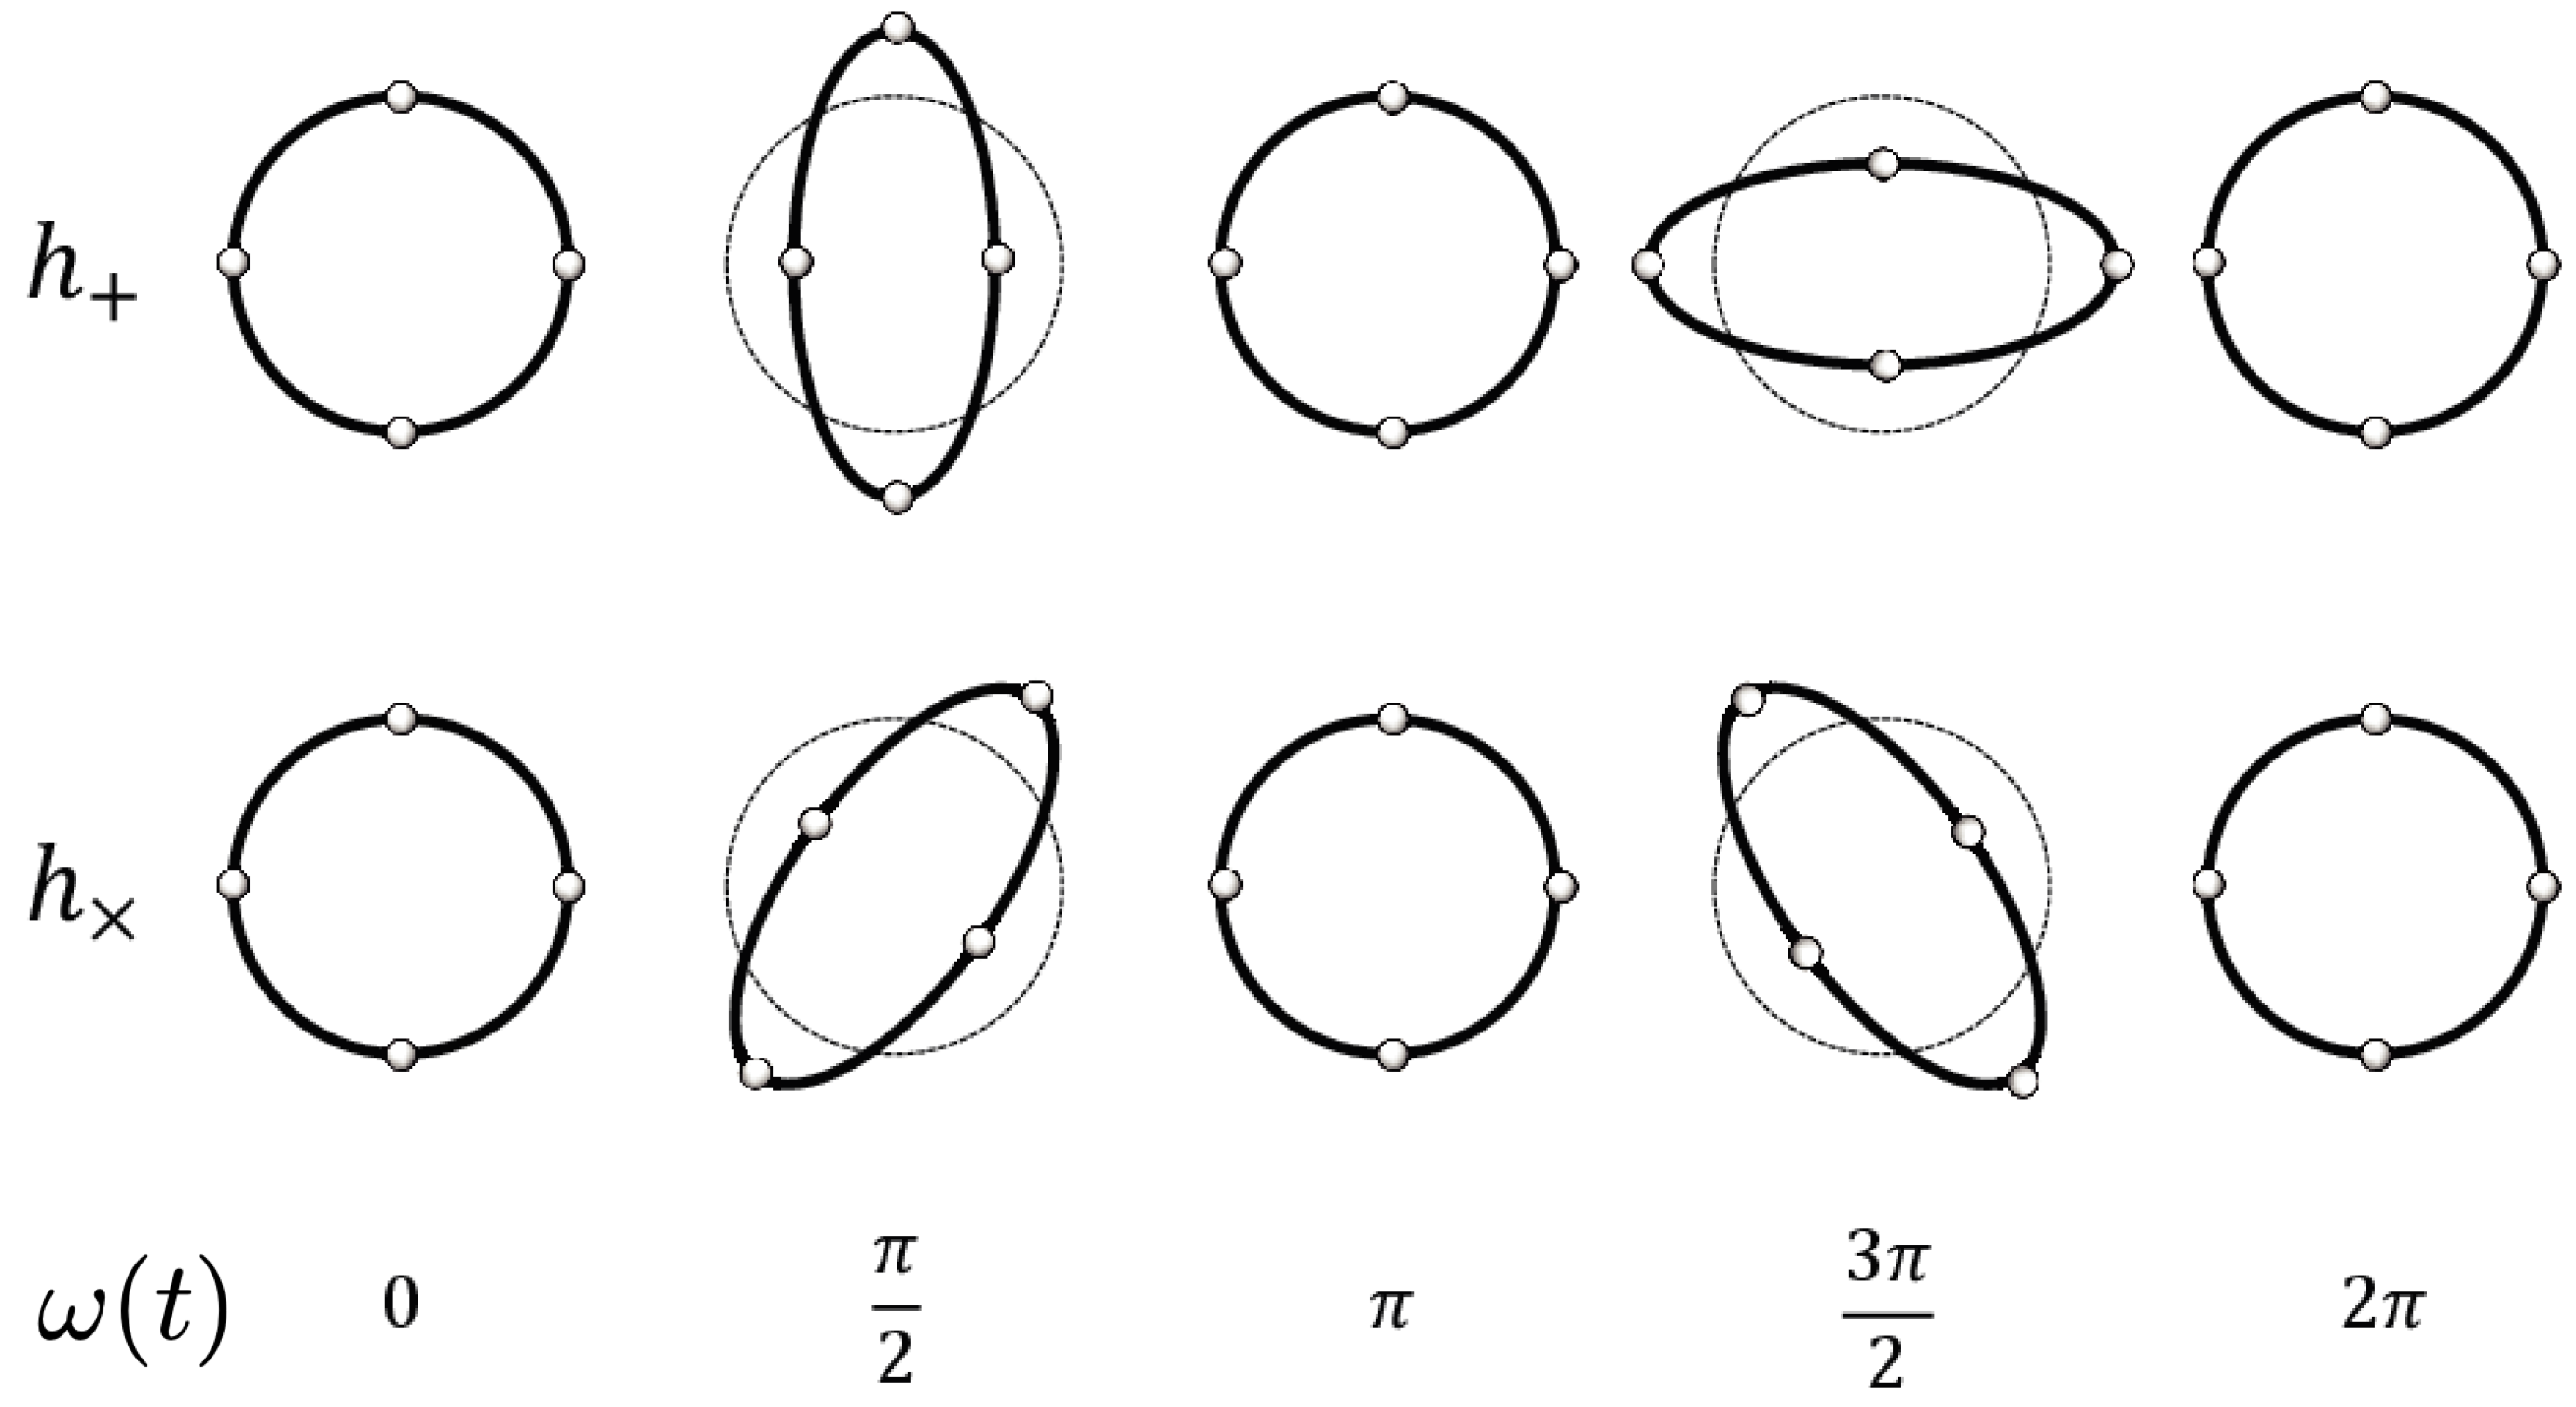
\includegraphics[scale=1]{ring}
                \centering
                \caption{The effects of plus and cross polarization on a ring of test masses. The plus polarization alternately compresses and stretches the x- and y-separations. The cross polarization has the same effect only rotated by  $\ang{45}$.}
                \label{fig:ring}
                \end{figure}

\section{Response of an interferometer to a gravitational wave}

        Interferometers are sensitive to the relative difference between two distances, the so-called strain \cite{6} .
        Suppose we have an interferometer with its arms pointing along the unit vectors $u^i$ and $v^i$. The strain $h(t)$ is given by
                \begin{equation}
                	h(t) = {1 \over 2} (h_{ij}u^iu^j - h_{ij}v^iv^j) = D^{ij}h_{ij}(t)
                \end{equation}
        where $D^{ij}$ is referred to as the detector tensor and is given by
                \begin{equation}
                	D^{ij} = {1\over 2} (u^iu^j -v^iv^j)
                \end{equation}
        As the expression for $h(t)$ is linear in $h_{+}$ and $h_{\times}$, one can also write
                \begin{equation}
		 \label{beampattern}
                	h(t) = F_{+}h_{+} (t) + F_{\times}h_{\times}(t)
                \end{equation}
        where $F_{+,\times}$ are called the beam pattern functions. Suppose we have a detector
        with arms that are perpendicular to each other, one pointing in the x-direction and the other
        in the $y$-direction in a Cartesian coordinate system. This detector frame, denoted by $(x,y,z)$,
        is generally different from the GW coordinate system, denoted by $(x^\prime,y^\prime,z^\prime)$, where the source
        is conveniently described. To account for such a difference, we first note that when the plus
        and cross polarisations are not equal in strength, we can rotate the coordinate system by
        an angle $\psi$ around the $z^\prime$ axis so that the $x^\prime$ and $y^\prime$ axes
        coincide with the mayor and minor axis of the associated ellipse. \\
        In going from the GW frame to the detector frame, we can rotate the GW frame by
        an angle $\theta$ around the $x^\prime$ axis and an angle $\phi$ around the $z^\prime$ axis,
        where the angles $(\theta, \phi)$ denote the direction of propagation of the GW in the detector frame.
        Applying these three rotations, the beam pattern functions for a detector with perpendicular arms are given by
                \begin{align}
                F_{+}^{\ang{90}}& = {1 \over 2} (1 + \cos^2 \theta)\cos 2\phi \cos 2 \psi - \cos \theta \sin2\phi \sin2\psi \\
                F_{\times}^{\ang{90}}& = {1 \over 2} (1 + \cos^2 \theta)\cos 2\phi \sin 2 \psi + \cos \theta \sin2\phi \cos2\psi
                \end{align}

\section{Non-stationary transient noise sources}
	
	The various noises of the detector can be conveniently characterized by a spectral strain
        sensitivity with dimensions of $1/\sqrt{Hz}$, as we explain in this section. 
        The detector output $s(t)$ is composed of instrumental noise $n(t)$ arising from
        naturally occurring random processes and a potential strain signal $h(t)$
                \begin{equation}
                	s(t) = n(t) + h(t)
                \end{equation}
        The detection problem then becomes how to distinguish $h(t)$ from $n(t)$ when $h(t) << n(t)$.
        In a way, $n(t)$ provides a measure of how small an $h(t)$ we can detect.
        Thus we take $n(t)$ as the detector’s noise and have a convenient way to
        compare performances of different detectors.
	The instrument response $s(t)$ can be also expressed as a convolution of the antenna patterns 
	with the two GW polarizations $h_{+}, h_{\times}(t)$:
		\begin{equation}
			s(t) = n(t) +  F_{+}h_{+} (t) + F_{\times}h_{\times}(t)
		\end{equation} 
	The antenna patterns depend on the frequency and sky location of the source; 
	for wavelengths that are large compared to the detector, the antenna patterns are simple quadrupoles \cite{19}.
	The information contained in the time series is usually represented in the Fourier domain 
	as a strain amplitude spectral density, $h(f)$. \\
	This quantity is defined in terms of the power spectral density $S_s(f) = \tilde s^{*}(f) \tilde s(f)$
	of the Fourier transform of the time series:
		\begin{equation}
                	\tilde s(f) = \int^{\infty}_{-\infty} e^{-2 \pi ift} s(t)dt
		\end{equation}
	The strain amplitude spectral density is then defined as $h(f) = \sqrt{S_s(f)}$.
	Noise is categorised as either displacement noise, which directly moves the suspended mirrors
        causing a differential change in the arm cavity lengths, or as sensing noise,
        which appears in the readout signal but is not caused by a GW. \\
        We describe the principal noises that dominate the limits of our sensitivity, (Fig.$\ref{fig:noise2}$).
		\begin{figure}[H]
                        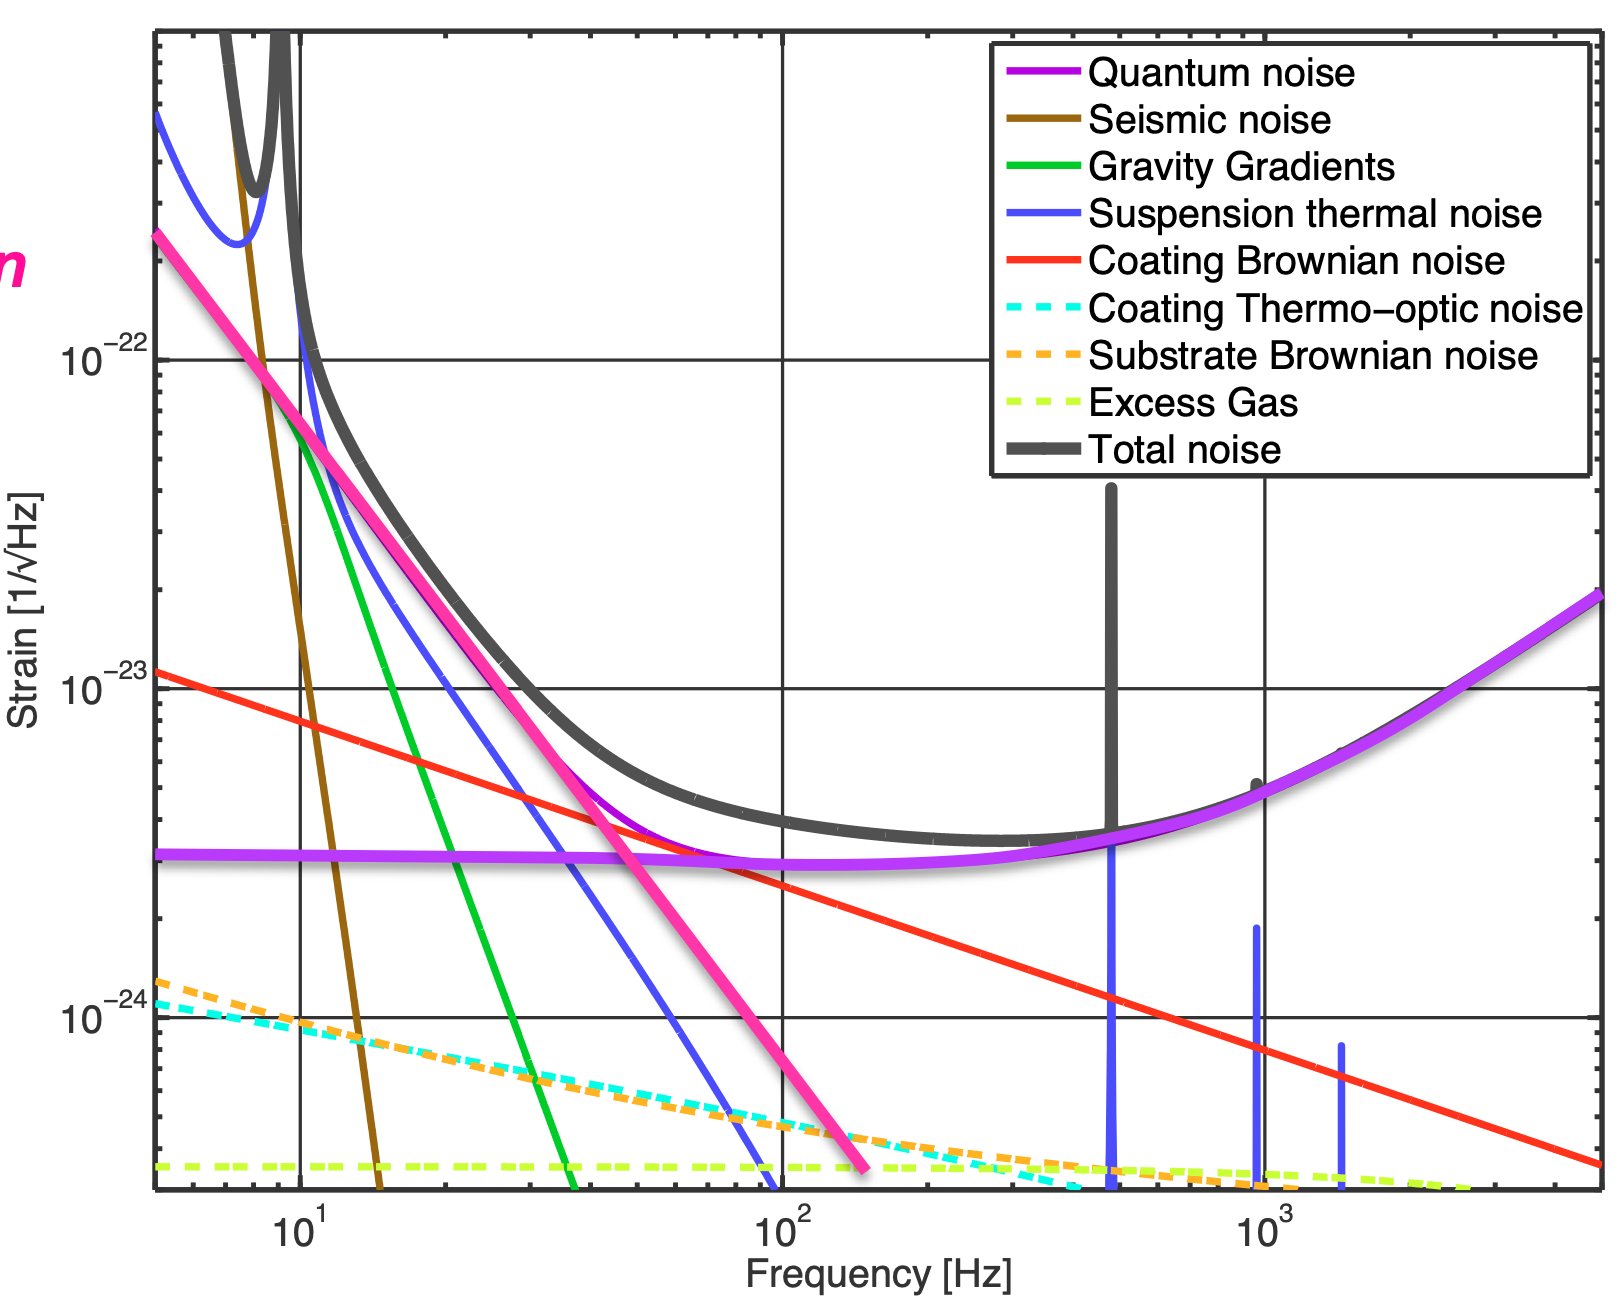
\includegraphics[scale=0.3]{noise2}
                        \centering
                        \caption{The strain equivalent spectral amplitudes $\sqrt{S_n(\omega)}$ of several noises couple to the detector. Most relevant contributions comes from quantum noise and from thermal noise of mirror coating and suspensions. Seismic noise dominates below 10Hz}
                        \label{fig:noise2}
                \end{figure}
        At lower frequencies, up to 10Hz, the main contribution to the global noise
        is due to vibrations of the ground which couple to the mirror motion, (Fig.$\ref{fig:noise2}$ brown line): 
	it shakes the optics and produces strain signals that mask GW signals. 
        This seismic noise is caused by earthquakes, weather and human activity.
        To reduce the potential movements of the optical elements,
        the mirrors are isolated using an advanced suspension system. \\
        At frequencies where the seismic motion has been sufficiently reduced,
        between 10Hz and 500Hz, the random Brownian motion of the molecules on the surface of the mirrors and wires dominates (Fig.$\ref{fig:noise2}$ red line). \\
        The thermal energy of the interferometer’s components induce vibrations both in the suspensions and in the mirrors.
        The nature of GW signal requires the sensitivity of the interferometric detectors
        to be extremely high in broad frequency band.
        Therefore, the power spectrum density of the thermal noise must be considered in the development of the detectors.
        The Fluctuation-dissipation Theorem relates the spectrum of the thermal noise to the amount of dissipation
                \begin{equation}
                	S_{n}(\omega) = - {{4k_bT} \over {\omega}} Im[H(\omega)]
                \end{equation}
        From this equation is possible to state that the energy of fluctuations has a frequency dependent distribution;
        $H(z)$ is the transfer function of the system, it is a mathematical function that models the device’s output, defined as
                \begin{equation}
                	H(x) = {1 \over {iWZ(\omega)}}
                \end{equation}
        In which $Z(\omega)$ is the impedance of the system in the frequency domain that can be computed as the ratio
        between the Fourier components of the generalised force $\tilde F(\omega)$ and the response of the system $\tilde X(\omega)$
                \begin{equation}
                	Z(\omega) = {{\tilde F(\omega)} \over {i\omega \tilde X(\omega)}}
                \end{equation}
        In the case of an harmonic oscillator, the noise spectral density is
                \begin{equation}
                	S_n(\omega) = {{4k_bT} \over {m\omega}} {{{\omega_0}^2 \phi(\omega)} \over {(\omega^2-{\omega_0}^2)^2 + {\omega_0}^4 \phi^2(\omega)}}
		\end{equation} 
	Generally, thermal noise can be reduced decreasing the dissipation with monolithic suspensions and better coatings
        other than lowering the temperature using criogenic payloads as it is done in KAGRA.
        Quantum mechanics limits the precision at which the test mass positions can be determined. \\
        At high frequencies, photon shot noise limits the sensitivity, 
	while at low frequencies it is limited by radiation pressure.
        The photon shot noise is produced by the natural fluctuations in the rate of photons arriving at the photodiode,
        that follow a Poisson process. The noise will decrease with increasing laser power,
        recycling cavity gain, arm cavity gain, and arm length.
        The corresponding noise spectral density is
		\begin{equation}
                	S_n(\omega) = \Bigg({{\lambda_{laser}} \over {4 \pi L}}\Bigg)^2 {{2 \hbar \omega_{laser}} \over {P}}
                \end{equation}
        Radiation pressure noise is associated with the photons from the laser striking the mirror
        and causing a force on the mirror. Of course, increasing the laser power to combat shot noise
        will actually result in an increase of radiation pressure.
                \begin{equation}
                	S_n(\omega) =  {{32 \hbar \omega_{laser}P} \over {(4MLc \pi^2 f^2)^2}}
                \end{equation}
        This is an example of the Heisenberg’s Uncertainty Principle, which says that the knowledge
        of the position and the momentum of a body is restricted from the relation $\Delta x \Delta p \geq \hbar$. 
        The high laser power required to determine the position of the test masses exerts
        a fluctuating radiation pressure which perturbs the test mass positions. 
        The minimun noise level is called Standard Quantum Limit (SQL) and sets a fundamental limit
        on the sensitivity of beam detectors, contributing to the noise as
                \begin{equation}
                	S_n(\omega) = {{2 \hbar} \over {M(\pi f L)^2}}
                \end{equation}
        Moreover, the presence of residual gas in the beam tubes would worsen the performance
        of the mirrors and of the laser; for this reason the vacuum system is maintained at a pressure
        of below $10^{-6}$Pa and the noise curve of the interferometer includes only
        the most dominant residual gas component, hydrogen, at a pressure of $10^{−7}$ Pa. 
		\begin{figure}[H]
                	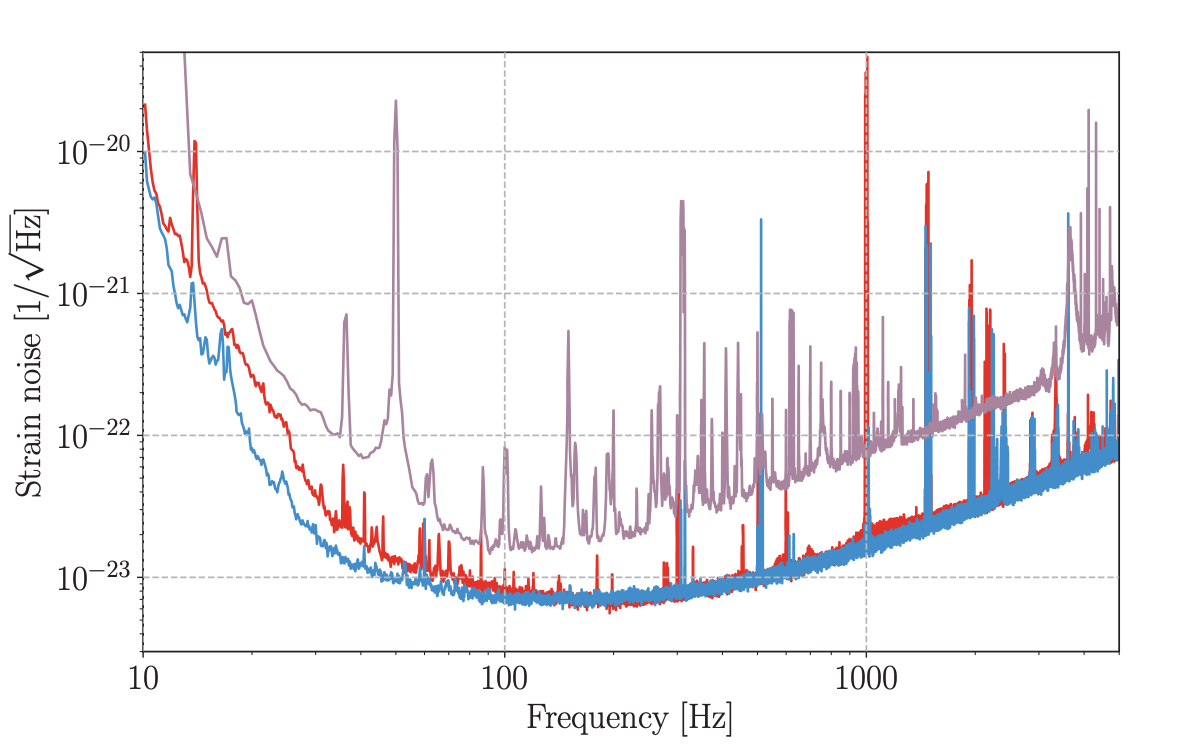
\includegraphics[scale=0.6]{noise1}
                	\centering
                	\caption{Amplitude spectral density of the total strain noise  of the Virgo, LHO, and LLO detectors. The curves are representative of the best performance of each detector during O2 \cite{13}.}
                	\label{fig:noise1}
                \end{figure}

\subsection{Sources}
\label{sec:sources}

	There are four different classes of physical sources 
	that are potential sources of GWs 
	of sufficient amplitude to be detectable 
	by current or theorised GW detectors. 

\subsubsection{Coalescing compact binaries}

	Compact binary star systems, in which each member is a NS or BH, 
	are currently the only observed sources of GWs.
	They are an ideal source for ground based GW detectors, 
	as their compactness allows their orbital separation to become 
	small enough before they merge for them to emit GWs in the detectors sensitive frequency band.
	If one of the components of the binary is a NS 
	then there may be an electromagnetic counterpart to the GW signal \cite{20}. 
	The loss of energy from the system will cause the orbital radius to decay, 
	the frequency to increase, and the amplitude of the radiation to increase, 
	producing a distinctive chirp-like signal. 
	Eventually, the two objects will be close enough to merge together, 
	and the new single object will pulsate in an excite state as it tries to return to equilibrium \cite{21}. 
	If the remanant is a BH, this phase is known as the ringdown phase and it is well-modeled as a series of quasi-normal modes. 
	As the form of the gravitational radiation can be predicted allows 
	a more sensitive search to be performed: knowing the form of the signal 
	that is being search for allows powerful matched filtering techniques 
	and signal consistency tests to be used in the attempt to detect such signals.


\subsubsection{Bursts}

	A burst of GWs is an event that releases a large amount 
	of gravitational energy over a very short period of time, typically less than a few seconds.  
	Astrophysical events that are believed to result in a transient signal 
	include gamma ray bursts and supernovae explosion as well as the final stages of a coalescing binary. 
	GW signal with a partially modelled or unknown waveform, 
	this may be due to unknown or complicated physics, or the source may be something totally unpredicted. 
	The matched filtering is not a useful technique to search for this type of signal, 
	as the waveform of a GW burst signal is unknown \cite{3}. 
	Searches for GW bursts typically search for excess power that occurs coherently between multiple detectors.  
	Even with no knowledge of the source of a GW signal, 
	it is still possible to estimate some of the source parameters. 
	Searches for GW bursts typically give estimations of the duration, 
	amplitude and frequency of the source. \\
	An estimation of the sky position is given by measuring the difference 
	in arrival time between different detectors. 
	If the distance to the source is known, 
	perhaps through an electromagnetic counterpart, 
	then it is possible to estimate the energy of the source. 


\subsubsection{Continuous Sources}

	A periodic source is a source that emits at constant or nearly constant frequency.
	The prototypical source of continuous GWs is high frequency rotating NSs 
	with a non-axial deformation or low frequency binary systems 
	composed of white dwarfs or BHs far from merger. 
	These sources should be present throughout the operational lifetime of a detector, 
	so the greater the observation time, the better the sensitivity to periodic sources becomes. 
	Spinning NSs will lose energy and spin down over time, 
	and this energy loss is due to a number of different mechanisms, 
	including emission of gravitational radiation \cite{3}. 
	To emit a continuous GW with characteristic amplitude, 
	a NS must have a non-axisymmetry in the crust. 
	The radiation amplitude is proportional to the crucial parameter $\epsilon$, 
	the fractional asymmetry that is proportional to the mass of the bump on the surface. \\
	As NSs emit electromagnetic radiation, 
	it is possible to target searches of GWs for NSs with positions, 
	frequencies and spin-downs known from X-ray, radio and gamma-ray observations. 
	Examples are the Crab and Vela pulsars. 
	Continuous GWs have not yet been detected, 
	but current searches have produced upper limits for their emission. 
	Upgraded interferometers in LIGO could set an upper limit on  
	$\epsilon$ of order $10^{-6}$ for sources at $\sim10$ kpc, 
	and explain how a NS can be distorted to give a value of $\epsilon$ that is interesting as a GW source. 
	Whatever the mechanism generating the distortion, 
	it is clear that  $\epsilon$ will be small,
	so that $h \sim 10^{-24}$ or smaller, which is quite weak. 
	Measuring these waves will require
	coherently tracking their signal for a large number of wave cycles, 
	which is actually quite difficult, 
	since the signal is strongly modulated by the Earth’s rotation and orbital motion.\\
	Searching for periodic GWs means demodulating the motion of the detector, 
	a computationally intensive problem since the modulation is different for every sky position \cite{4}. 
	Unless one knows in advance the position of the source, 
	one needs to search over a huge number of sky position "error boxes”.

\subsubsection{Stochastic background}

	Stochastic backgrounds are “random” GWs, 
	arising from a  number of sources that overlap 
	in time and frequency that are not individually resolvable \cite{22}. 
	The sum of the signals at any given time and frequency will have 
	a random pattern that may be analyzed statistically but not predicted precisely.
	A particularly interesting source of stochastic waves is the dynamics of the early Universe, 
	which could produce an all-sky GW background, 
	similar to the cosmic microwave background. \\ 
	However, to measure waves from this epoch, 
	we would need much more sensitive detectors than the ground-based interferometers available.
	Stochastic backgrounds are usually idealized as being stationary, 
	isotropic and homogeneous and because of their random nature they look just like noise \cite{4}.	
	Another possible background could come from astrophysical sources. \\ 
	These possible sources include a population of rotating NSs 
	and a population of white dwarf binaries that would be important mostly for a space-based interferometers such as LISA. 

%----------------------------------------------------------------------------------------------------------------------------------------------------------------------------------------------------------
\chapter{Data Analysis for Coalescing Binary Systems}
\label{ch:datatools}
\fpg{Giri di correzione: 1.}%
	One of the tasks of GW data analysis is to extract GWs signal 
	buried into noisy interferometric strain data, hence achieving GW detections.
	The techniques involved in this proces depend on the type of source.
	GW searches from the inspiral, merger and ringdown phases of compact binary systems 
	are based on two broad techniques: 
	modeled searches which use theoretical waveforms for the GW emitted by such systems 
	as predicted by general relativity, and 
	unmodelled (or burst) searches which assume minimal information about these waveforms \cite{23}.
        This chapter provides a basic overview of the main data analysis ingredients needed to perform a modelled GW search:
        matched filtering, template banks, evalution of a candidate's significance, measure of the sensitivity of a search.

\section{Matched Filtering}
\label{sec:matched_filtering}
	Although signals from coalescing binaries will most probably not stand above the broadband noise of the detector, 
	their detection is possible by the use of matched filtering, 
	which takes advantage of the fact that the waveform can be fairly well predicted. 
	As we will see, this technique is the optimal detection strategy when searching for GWs
        with well understood waveforms in Gaussian noise.

	The filtering procedure involves correlating the detector output 
	with a copy of the expected waveform, 
	called template.
	A real detector operates over a finite frequency band, 
	and acquires data at a finite sample rate \cite{24}. 
	In this case, the noise power spectrum $S_n$ 
	may be taken to be infinite outside the bandwidth of the instrument, 
	effectively restricting the range of integration to lie between $[-f_N, f_N]$, 
	where $f_N$ denotes the Nyquist frequency $f_N = 1/(2\Delta t)$, 
	and $\Delta t$ is the time between successive data samples.   \\
	The measured detector strain amplitude, $s(t)$, may or may not contain a signal,
	thus it will be composed of $n(t)$, the real strain-equivalent noise
        produced by fluctuations within the detector and its environment, 
	and possibly a GW of known form, $h(t)$
                \begin{equation}
                \label{eq:strain}        
			s(t) = h(t) + n(t)\,.
                \end{equation}
        When no signal is present,   		
		\begin{equation}
                        s(t) = n(t)\,.
                \end{equation}
        The aim of the match filtering is to look for a filter function to process the data,
	the output of which will be large when a signal is present and small otherwise. 
        If the waveform, $h(t)$, is embedded in stationary Gaussian noise with zero mean and one-sided power-spectral density (PSD) $S_n(f)$,
        the optimal filter takes the form $\tilde h_{template}/S_n$, where $\tilde h_{template}$
        is the frequency domain waveform template that approximates the real signal to the best of our knowledge.
	This optimal filter may be cross-correlated with the data over the detector frequency band to search for GW
        signals.  The output of this filtering operation may be viewed as a weighted inner product in the frequency domain, 
	between the data and the template, where the weight is the inverse PSD of the detector:
		\begin{equation}
 			(s|h)(t) = 4Re \int^{f^{high}}_{f^{low}} {{\tilde s (f) \tilde h^{*}_{template}(f)} \over {S_n (f)}} e^{2 \pi ift}df\,, 
		\end{equation}
	where the frequency limits $f_{low}$ and $f_{high}$ are determined by the detector bandwidth
	and $\hat s(f)$ denotes the Fourier-transformed detector data, defined as
		\begin{equation}
			\tilde s(f) = \int^{\infty}_{-\infty} s(t) e^{-2i \pi tf} dt\,.
		\end{equation}
  
\subsection{Signal-to-noise ratio}

	Finding the form of the filter which will optimally extract the signal from the noise,
        means locating the maxima of the output of the matched filter, $(s|h)(t)$, 
	over the arrival time and phase.
        One can therefore set a threshold value such that values of the matched filter 
	above it would indicate a signal candidate while values below would indicate the absence of signals. \\
	The filter output can be normalized by the variance of the optimal filter, $\sigma^2$,
	which is an estimate of the uncertainty in a measurement of $(s|h)$ due to the detector noise:
                \begin{equation}
                        \sigma^2 =4 \int^{f^{high}}_{f^{low}} {{|\tilde h_{template}(f)|^2} \over {S_n(f)}}df
                \end{equation}
 	The normalized output of the optimal filter is a new thresholding statistic and can be defined as  
	the signal-to-noise ratio (SNR), the ratio of the observed filter output to its,
        expected or observed, root-mean-square fluctuations \cite{24}:
                \begin{align}
                        \rho(t) &= {{| (s|h) |} \over {\sigma_{h}}} \\
                             &= {{(\tilde s|\tilde h_{template})} \over {\sqrt{(h_{template}|h_{template})}}}\,.
                \end{align}
        The value of the SNR will then be proportional to the amplitude of the signal buried in the noise.
	The smart choice for a threshold that can be set on this value is such that
	it can admit as many signals as possible, while still keeping the false alarm rate low. 

\subsection{Matched filtering for compact binary coalescence signals}
\label{subsec:mfcbc}
	An interferometric detector is sensitive to a linear combination 
	of the two GW polarizations \cite{26}: 
                \begin{equation}
                h(t) = F_{+}h_{+} (t) + F_{\times}h_{\times}(t)\,,
                \end{equation}
	where $F_{+}$ and $F_{\times}$ are the two antenna response functions of the detector, 
	which depend on $\theta$ and $\phi$, 
	the angular coordinates of the source sky position with respect to axes defined by the interferometer arms. 
	Due to the nature of GW signals from the inspiral stage of compact binary coalescences (CBCs), 
	it follows that the phase evolution of the cross polarization is $\ang{90}$ out of phase with the plus polarization:
		\begin{equation}
			h_{+}(t) = A(t) \cos (\phi (t))
		\end{equation}
		\begin{equation}
			h_{\times}(t) = A(t) \sin (\phi (t))  
		\end{equation}
	where $A(t)$ is the amplitude evolution of the signal 
	and $\phi(t)$ is the phase evolution of the signal. 
	The Fourier transform of the two polarization are related by $\tilde h_{+} = i\tilde{h}_{\times}$, 
	which means that the inner product between the two orthogonal polarisations is zero 
		\begin{equation}
			(h_{\times}|h_{+}) = 0
		\end{equation}
	Hence, when filtering  $s = (Xh_{+}/\sigma_{h}) + (Y h_{\times}/\sigma_{h})$ 
	with the templates $h_{+}$ and $h_{\times}$, we obtain the matched-filter real-time series
		\begin{equation}
			z_{+} = X\sigma_{h}
		\end{equation}
		\begin{equation}
			z_{\times} = Y \sigma_{h} 
		\end{equation}
	This leads to the definition of the two-phase filter, 
	which has twice the degrees of freedom of a single-phase filter:
		\begin{equation}
			\rho = {1 \over \sigma_h} \sqrt{|z_{+}| ^2+ |z_{\times}|^2}
		\end{equation}
	The bonus of extracting information from both polarizations of the GW 
	comes at the cost of increasing the expectation value of $\rho$ when there is no signal present. 
	For a detector output that includes a signal at distance $D_{eff}$, 
	$s(t) = n(t) + (D_{eff}/1 Mpc)^{-1}h_{1Mpc}$, 
	a biased estimate of the effective distance for a given trigger 
	may be defined by combining the definition of the SNR with the template normalization $\sigma_h$:
		\begin{equation}
			\hat D_{eff} = {{\sigma_h} \over {\rho}}
		\end{equation}
	In reality, the parameters of astrophysical systems will not be known a-priori, 
	and searches must therefore be sensitive to signals at any location in the parameter space \cite{25}. 
	Performing the matched-filter calculation at every point in the full parameter space 
	would be computationally prohibitive, 
	and therefore a number of analytic approximations are used to reduce the size of the parameter space. 
	It is assumed that the ``extrinsic'' parameters of a GW signal --- 
	sky-location, source orientation, polarisation phase and distance --- 
	can all be absorbed by applying a constant phase-shift, 
	constant time-shift and a constant amplitude scaling to the observed waveform \cite{27}. 
	With these assumptions in place, 
	one can analytically maximise over an overall amplitude and phase of the signal, 
	and use an inverse Fourier transform to quickly evaluate the statistic as a function of time. \\
	The component masses and spins --- the intrinsic parameters --- 
	are searched over by repeating the search process with a well chosen discrete set of waveform models 
	with varying values of the component masses and spins, 
	known as the template bank \cite{27}. 
	Physically, these assumptions hold if one assumes that the sources being observed 
	have negligible orbital eccentricity, precession and contributions from higher-order modes 
	to the GW signal \cite{23}. 

\section{Template Banks}

	To perform a matched-filtered search that recovers compact binary coalescence signals
	with minimal loss of SNR over a given range of intrinsic parameters, 
	one must filter the data against a predetermined collection of waveform models: the template bank \cite{28}.
	The manifold of waveforms is a continuous space in the component masses and spins. 
	One may only to search over this manifold on a discrete points, 
	which have to be placed in such a way that any signal
	that has parameters in the targeted space will still produce an SNR 
	above threshold by matching with the ''losest'' template \cite{27}. \\ 
	In order to compute the distance between two templates with different parameter values, 
	one can create a metric over the parameter space and then compute an ``error'' between two waveforms.
	Two neighbouring templates can be defined as $h(f;\lambda)$ and $h(f;\lambda + \Delta \lambda)$,
        where $\lambda = \{\lambda_{intr}, \lambda_{extr}\}$ is the set of
        intrinsic (masses and spins) and extrinsic (time and phase shifts) template parameters.
	The overlap of two waveforms, defined as the inner product inversely weighted by the detector one-sided  PSD $S_n(f)$, 
	can be written as  
		\begin{equation}
			(h_i| h_j)  \equiv 4 \int_{0}^{\infty} df {{\tilde h_i(f) \tilde h^*_j(f)} \over {S_n(f)}}.
                \end{equation}
	The normalised overlap between the two waveforms is given by
		\begin{align}
			(\hat{h}_i|\hat{h}_j)& = {{(h_i|h_j)} \over {\sqrt{(h_i| h_i)(h_j| h_j)}}}\,.
		\end{align}
	As the template waveforms are defined up to an overall normalization, 
	it is customary to work directly with the normalized $\hat{h}_i$'s. \\
	The match is then defined as
		\begin{equation}
			\mathcal{M}(\lambda, \Delta \lambda) \equiv \max_{\Delta \lambda_{extr}} (\hat h(f;\lambda), \hat h(f;\lambda + \Delta \lambda))
		\end{equation}
	The match is maximised only over the two extrinsic parameters of a template, 
	because waveforms related by time and phase offsets
	are described by the same template, 
	since all possible coalescence times and phases are searched for \cite{29}. \\
	This expression can be Taylor-expanded about $\Delta \lambda = 0$:
		\begin{equation}
			\mathcal{M}(\lambda, \Delta \lambda) \simeq 1 - g_{ij} \Delta \lambda^i \Delta \lambda^j\,,
		\end{equation}
	where 
		\begin{equation}
			 g_{ij} \equiv -{1 \over 2} {{\partial^2\mathcal{M}} \over {\partial  \Delta \lambda^i  \partial \Delta \lambda^j}}\vert_{\Delta \lambda = 0}
		\end{equation}
	can be interpreted as a metric in the waveform manifold.  A commonly used quantity related to this metric
	is the mismatch between two templates $MM = (1 − \mathcal{M})$.
	Any mismatch between signal and template leads to a loss in SNR, 
	and to a down-weighting by the signal-based vetoes, see Sec. $\ref{subsec:chi_square_test}$. \\
	When constructing a template bank, this mismatch can be viewed as the means
	to compute the proper distance in the waveform space:
		\begin{equation}
			ds_{ij}^2 = 1 − \mathcal{M} = g_{ij} \Delta \lambda^i \Delta \lambda^j\,.
		\end{equation}
	This proper distance should be chosen to guarantee that the loss in SNR due to the mismatch 
	between template and signal does not jeopardize the detectability of the signal \cite{30}.

\subsubsection{Fitting factor}
\label{subsec:fittingfactor}
	The standard measure used to determine the set of waveform models to used in a
        search is the fitting factor, $FF$.
	The fitting factor quantitatively describes the ``closeness'' of 
	the true signals to the template manifold, in terms of the fraction of 
	SNR obtained when filtering 
	the data with an approximate family of templates \cite{31}. 
	To quantify the bank coverage, usually Monte-Carlo simulations are carried out   
	to compute the distribution of fitting factors of the templates in the bank against 
	a set of injected signal waveforms with randomly chosen parameters \cite{32}. \\
	The fitting factor, $FF$, of a template bank with respect to an injected signal $h_{*}$ 
	is defined as the maximum value of match over all the templates:
		\begin{equation}
			FF(h_{*}) = \max_\Lambda \mathcal{M}(\tilde{h}_{*}, \tilde{h}(\Lambda))
		\end{equation}
	assuming that the signal model is the same for both templates and injections. 
	The fractional loss of SNR in capturing the signal 
	$h_{*}$ with the template bank is $1 - FF(h_{*})$.
	If the fitting factor is less than unity, the signal lies outside the parameter space, 
	and the fitting factor represents the cross-correlation between 
	the signal and its nearest template in the waveform parameter space \cite{33}. 
	This loss arises from the discrete placement of the templates. 
	Because binaries are, on large scales, uniformly distributed in space 
	and because the signal strength scales inversely with distance, 
	the fraction of events retained is approximately $FF(h_*)^3$. \\ 
	Therefore it is desirable that the template bank is constructed such that 
	no putative signal anywhere in the parameter space
	has a FF value less than the minimal match. 
	A bank is said to be effectual if it can satisfy this condition.
	It has become conventional to set $FF = 97\%$ as a reasonable goal when building a template bank, 
	as this translates into a $10\%$ loss of events \cite{33}.

\subsubsection{Frequency bound}

	An algorithm that most efficiently covers the parameter space relies on the choice of a coordinate system, 
	in which the metric is as flat as possible across the space \cite{34}.
	In computations with the two-mass-parameter waveforms, 
	the best coordinates to use on the parameter space are not the two masses, 
	but rather the inspiral times, chirp times, from some fiducial frequency to final merger, 
	as computed at Newtonian and first post-Newtonian order. 
	The metric components are slowly varying over the parameter space, 
	when expressed in as dimensionless chirp times. 
        The lower frequency cutoff $f_L$, which essentially determines the size of the parameter space
        of chirptimes and plays a crucial role in the computational resources required
        to process the data through the template bank \cite{30}, and is not itself a parameter to search for. \\
        However, it affects the length of the signals
        (therefore, the parameter space to be covered) and the SNR extracted.

\subsection{Template placement}

	The computational cost of any GW search
	 is directly proportional to the number of templates used \cite{28}.
	It is therefore vital to have a method that enables one 
	to place a template bank using as few templates as possible. \\ 
	Two broad classes of template-placement algorithms 
	have been developed in the literature. 

\subsubsection{Stochastic placement}

	Stochastic methods place templates, 
	that are randomly drawn from an initially chosen distribution, 
	at random points in the parameter space.
	The bank is gradually built by comparing the newly drawn waveform
	with previously accepted templates, 
	and keeping only the ones that are sufficiently far away 
	from the ones already in the bank.
 	Those that are too similar to at least one existing waveform are discarded \cite{35}.
	This procedure continues until the pre-set convergence threshold is reached, 
	resulting in a final saturated template bank.
	The threshold is measured from the ratio of rejected templates over the total number of template candidates.
	Stochastic placement, however, has the shortcoming that 
	a large number of trial waveforms needs to be drawn and generated before convergence is achieved 
	(many more than the required number of templates in the bank). 
	This method also tends to over-cover the parameter space, 
	in the sense that the average template density is higher than optimal at fixed minimum match. \\
	Furthermore, the construction of a stochastic template bank 
	can be computationally demanding since, in principle, 
	each new proposed template needs to be compared 
	with the previously chosen templates \cite{36}. 
	This problem becomes particularly acute 
	the closer the bank gets to saturation. 
	The computational problem also becomes especially demanding 
	when precession effects are considered as these additional degrees 
	of freedom require a large number of templates. \\
	It is therefore important to consider methods to optimise the template bank construction, 
	specifically finding ways of improving effectualness for a given number 
	of templates and reducing the computational cost. 

\subsubsection{Geometric placement}


	A different method to construct the bank is geometric placement:
	this means building a flat, linear space in such a way that embeds the space of physical waveforms. 
	Hence, a crucial point is to identify a set of coordinates 
	in which the parameter space metric is almost constant: 
	the Euclidean distance in this space coincides with the matched-filtering overlap 
	between waveforms, making these coordinates naturally suited to define a regular lattice. 
	The minimal match determines the choice of spacing of the discrete template parameters, as shown in Section 3.2, 
	and therefore the number of discrete templates in the family.
	The most significant drawback of such banks is the amount of fine-tuning required 
	in order to cover ``holes'' across local patches because of the misalignment 
	of the cells arising from the variation of the metric \cite{29}. 

\subsubsection{Hybrid placement}

	In practice, a combination of the two methods is often a better strategy. 
	For example, one can place templates geometrically at low masses 
	and stochastically at high masses, or one can use many small patches 
	with regularly spaced templates, which are themselves placed stochastically 
	to cover the entire parameter space \cite{29, 34}. 

\subsubsection{Spins of compact objects}

	The processes that lead to the formation of a compact binary
	depend sensitively on a number of poorly constrained parameters, 
	such as the typical stellar metallicity at formation, 
	the distribution of supernova kicks, 
	and the binding energy of the common envelope. 
	There are two main channels through which compact objects can be formed:
	the coevolution of two massive stars in a binary and 
	the dynamical capture of two preformed compact objects 
	in dense stellar environments such as globular clusters \cite{37}. \\	
	It is thought that compact binaries formed by dynamical capture 
	are more likely to have component spins
	at large angles with respect to the orbital angular momentum, 
	while those formed by common evolution are more likely to have 
	spins that are nearly aligned with the orbital angular momentum.
	Present observations clearly indicate the potential for large spins 
	on BHs in binaries, possibly close to the Kerr limit $|\mathbf{S}/m^2| = |\mathbf{\chi}| = 1$.
	Very few measurements of the angles between the spins and 
	the orbital angular momentum exist from electromagnetic observations. 
	In some cases, one can measure this spin misalignment via GW emission, 
	as misalignment leads to precession of the orbital plane, 
	which appears as phase and amplitude modulations in the observed signal. \\
	Almost all searches for GWs from coalescing compact binaries 
	using the data of first generation interferometers 
	have used templates that neglect the spins of the compact objects \cite{32}.
	This was primarily motivated by the sensitivity of the initial LIGO and Virgo detectors:
	because the sensitivity band started above 40 Hz, 
	including spin effects greatly increased the number of templates to be searched over, 
	and the search performed, on average, no better than non spinning searches, 	
	as the increased degrees of freedom in the signal space picked up extra noise noise transients, 	
	increasing the false alarm rate \cite{32, 38}. \\ 
	However, the Advanced LIGO and Virgo detectors are sensitive to frequencies above 10–20 Hz, 
	therefore they can observe the inspiral from much larger orbital separations, 
	resulting is significantly longer observed GW signal \cite{23}. 
	Proper consideration of the spin effects is essential in the advanced detector era, 
	as there might be astrophysical systems that are entirely missed by non-precessing searches.
	Neglecting the spin effects can cause a much larger dephasing of the template with the signal, 
	and hence considerable loss of SNR. \\
	Currently, waveform models with spins (anti)aligned with the orbital angular momentum 
	are used in searches with Advanced LIGO and Virgo, 
	as it was demonstrated that aligned-spin templates accumulate more signals than noise \cite{27}. 
	While building a template bank with the geometric approach for these cases is feasible, 
	since a closed-form expression of the template-space metric can be computed, 
	this is not possible for binaries with generic spins. 
	This is due to the fact that, 
	if the spins are misaligned with the orbital angular momentum of the binary, 
	the spin-orbit and spin-spin interactions will cause the spins 
	(and hence the orbit) to precess. 
	The resulting dynamics as well as the GW forms are rather complex, 
	and the modelling requires solving a set of coupled ordinary differential equations \cite{39}. 
	The template placement is further complicated by the large dimensionality of the parameter space 
	(two mass parameters, five spin parameters, and two angles describing the orientation of the binary, in general). 
	Detecting highly precessing systems offers a better chance to 
	disentangle the various parameters that describe the source,  
	breaking degeneracies that exist between physical parameters 
	in the emitted GW signal.  
	This could allow for a better understanding of the nature and origin of these systems.
	Although the effect of precession on the GW signal is not fully captured 
	by aligned-spin templates, it has been demonstrated that non-precessing templates 
	are also effectual in detecting binaries with generic spins if the mass ratio is moderate 
	$(m_1/m_2 \leq 10)$; these spin effects can be also described by 
	a single reduced-spin parameter in an approximate way, 
	which makes the parameter space three-dimensional, 
	using the two masses and reduced-spin as variables \cite{32}. 
	
\section{Candidate ranking statistic}

 	Since the detector calibrated strain data contains both stationary, Gaussian noise
        and non-Gaussian noise transients of instrumental and environmental origin,
        matched filtering does not suffice as a detection statistic.
        Consistency checks are needed to mitigate the effect of noise transients,
        which can sometimes mimic signals of astrophysical origin,
        and to assign an accurate statistical significance to candidate signals.
        In order to eliminate the worst periods of detector performance, 
        data quality investigations are conducted by looking only at the detector behaviour,  
        which is analysed by monitoring environmental and instrumental channels \cite{40}.
        After removing data that is not suitable for astrophysical searches, 
        noise transients, glitches, of unknown origin could still be present in the data 
        and cause certain templates to produce high SNR values.
        To mitigate the effect of glitches, a gating procedure is applied:
        after identification of times impacting on the sensitivity of the search,
        the data are zeroed out around these times \cite{42}.
        Filtering the data with template banks generates a matched-filter SNR for each template in each detector;
        GPS times of local maxima that exceed the SNR threshold are recorded as triggers. 
        Waveform consistency tests are then needed to determine if the morphology 
        of a candidate signal is consistent with the expectation from the triggering template waveform.  If it is not,
        it is more likely to correspond to a noise transient.
	
\subsection{$\chi^2$ test}
\label{subsec:chi_square_test}
	For signals from compact binary mergers, one can construct $\chi^2$-test.
	A standard $\chi^2$-test consists in splitting the template into $p$ non-overlapping frequency bins 
	constructed so that each one contributes equally to 
	the SNR of a perfectly matching signal \cite{28, 41}. 
	The $\chi^2$ statistic compares the expected to the measured SNR in each bin as follows:
		\begin{equation}
			\chi^2_r = {1 \over {2p-2}}   \sum_{i=1}^{i=p} || \langle   s|h_i  \rangle -   \langle  h_i|h_i   \rangle ||^2\,,
		\end{equation}
	where $\chi^2_r = \chi^2/(2p-2)$ is the reduced chi-squared.  For real GW signals, this value should be close to unity, 
	meaning that the data is describing Gaussian noise with an embedded signal.\\
	The SNR returned by the matched filtering procedure is combined with the $\chi^2$-test result to produce a ranking statistic 
	that down-weights triggers caused by noise transients, the so-called reweighted SNR:
		\begin{equation}
		\begin{cases}
			\hat \rho &= \rho \hspace*{4.5cm}  \text{for} \hspace*{0.15cm}\chi^2_r \leq 1 \\
			\hat \rho &= \rho[{1 \over 2} (1 + (\chi^2_r)^3)]^{-1/6}  \hspace*{1.5cm}  \text{for} \hspace*{0.15cm} \chi^2_r > 1
		\end{cases}
		\end{equation}
                \fpg{Quello che segue riguarda i consistency tests, non i chi-square tests.} 
	This rewighting process makes sure that the distribution of $\hat \rho$
        in noise is close to that of SNR in Gaussian noise.
        Conversely, for a true astrophysical signal $\hat \rho \approx \rho$,
        as long as the mismatch between signals and templates is small.
 
\subsection{False Alarm Rate}
\label{subsec:far}
	After mitigating the effects of noise transients, the probability of remaining transients 
	occurring simultaneously in two detectors and producing a large joint 
	ranking statistic is reduced.
	In order to keep only the most representative trigger among all the triggers produced by a single inspiral signal or glitch, 
	a final clustering step is performed on coincident triggers, 
	by selecting those with the largest value of $\hat \rho$ 
	in each time window of $10$\,s. 
	Any other events in the same time window are discarded. 
	This ensures that a loud signal or transient noise artifact gives rise to at most one candidate event.
	In order to assess the actual significance of a candidate, 
	the false-alarm rate (FAR) of the search is computed as a function of the detection statistic.
  	Since it is not possible to isolate the detectors from GWs, 
	one cannot determine the FAR by \emph{directly} measuring the detector noise in the absence of signals and a different strategy must be used.
 	To estimate FARs, the data streams of the detecters are shifted in time relative to one another: generates a synthetic dataset in which the detector streams are uncorrelated.  The minimum time-shift offset is chosen to be larger than the time-coincidence window used to determine whether signals are observed with consistent parameters in the network.
	The coincidences resulting in this time-shifted data are then treated as a background noise sample.  They can either be coincident noise instances or coincidences between a noise transient and a signal.  The latter case generates a tail in the background noise distribution: when a signal candidate is present in the data, coincidences with it may be ignored to avoid the appearence of such tail.
	The time-shifting procedure is repeated multiple times in order to obtain a probability distribution for the joint detector ranking statistics \cite{44}. 
	Each coincident trigger is assigned a FAR given by the number 
	of background triggers $n_b(\hat \rho)$ with an equal or larger ranking statistic, 
	divided by the total time searched for time-shifted coincidences $T_b$
        \begin{equation}
          FAR = {{1 + n_b(\hat \rho)} \over {T_b}}\,.
        \end{equation}
        The inverse of the FAR (IFAR) quantifies the waiting time expected to be necessary before the candidate event in question is produced by noise:
        \begin{equation}
          IFAR = {1 \over {FAR}}
        \end{equation}

	To account for the noise background varying across the target signal space, 
	candidate and background events are divided into different search classes based on template length. 
	The significance of candidate events is measured against the background from the same class. 
	For each candidate event, one can compute the probabilty of finding one or more 
	noise background events in the observation time with a detection-statistic value above that of the candidate event.  This is given by 
		\begin{equation}
			p(\hat \rho) \equiv P(\geq 1 \hspace*{0.1cm}\text{noise event above}\hspace*{0.1cm} \hat \rho|T,T_b) = 1 - \exp\left[-T{{1+n_b(\hat \rho)} \over{T_b}}\right]\,,
		\end{equation}
	where $T$ is the observation time of the search and it multiplies the FAR in the exponential.
	If the detection-statistic value of a candidate event is larger 
	than that of any noise background event, 
	then the analysis places an upper bound on the $p$-value of that candidate. 
	

\section{Coincident and coherent searches}

	The two main detection strategies to search for GWs 	
	from a network of detectors are known as coincident and coherent.  
	In this section, we highlight differences between the two methods, 
	which will be both applied to analyse the O3 data, in Chapter $\ref{ch:datanalysis}$.  
	\fpg{Qui ci vuole una forward reference al capitolo con i risultati, cos\`i spieghi che hai fatto entrambi i tipi di searches.}

\subsection{Coincident analysis}
\label{subsec:coincident}
 	A coincidence analysis searches the data from individual detectors independently        
        and matches the candidate event lists of individual detectors for consistency,
        in the mass, spin, and time parameters of a GW signal.
	A coincidence is formed if the difference between the arrival times of two or more triggers from different detectors, 
	is less than the allowed time window:
	this window is taken as the maximum light travel time for GW between the sites plus a small, fixed amount to allow for timing errors. 
	For example, for the two-detector LHO-LLO network, signals must be seen in both detectors within a time difference of 15ms: 
	10ms maximum travel time between detectors and 5ms padding to account for timing errors. \\
        The benefits of this procedure are plenty: first it immediately eliminates the great majority of background noise 
	by rejecting any triggers which are not coincident in two or more detectors;
	secondly, it is not computationally expensive.
        The dominant cost of the search is in performing a matched filter 
        of the data against a bank of template waveforms (see, Section \ref{sec:matched_filtering}):
        this task is performed once per detector per template \cite{28, 45}. \\
	The {\ttfamily PyCBC} pipeline, used in Sec. $\ref{sec:pycbc00}$, 
	requires consistency of arrival time and template parameters (masses and spins) 
	between triggers in each of the detectors must be exactly the same,,
	since the same waveform should be observed in all detectors.
	The same template bank is used to filter data and produce triggers from each detector. \\
	When coincident events are found, they are then ranked by the quadrature sum of the reweighted SNR in each detector;
	for a two-detector network, the \textit{coincident} SNR is defined as
		\begin{equation}
			\hat{\rho}_{coinc}  = \sqrt{\hat{\rho}^2_1 + \hat{\rho}^2_2}.
		\end{equation}
	A confident detection is claimed when the false alarm probability of an event is computed,
	and the probability of an equally loud event being caused by noise is below a chosen threshold. 
	A statistical significance is assigned to candidate events by the FAR,
	calculated as a function of the detection statistic, $\hat{\rho}_{coinc}$,
	via analysis of time-shifted data, as already seen in Sec. $\ref{subsec:far}$. \\
	Single-detector triggers from one detector are time shifted with respect to triggers of the other detector;
	all such coincidences are recorded and assigned a ranking statistic, 
	to create a background data set that does not contain coincident GW signals.
	This time-shifting of the data is performed many times to obtain a representative estimate of the expected rate of background triggers. \\
	For every possible result of a given observation performed on the data with detection statistic $\hat{\rho}_{coinc}$, 
	a test statistic value, $p_b$ is assigned to measure the probability that the 
	there are one or more coincident noise events (false alarms) that have
	a detection statistic value greater than or equal to $\hat{\rho}_{coinc}$. 
	Given the knowledge of only GW data, one cannot be absolutely confident that 
	any given trigger is a signal rather than noise. 
	Therefore, p-values are computed under the null hypothesis: this assumes that candidate events 
	are caused by non-GW processes acting on and within the interferometers,
	even when loud signals are present in the data. \\
	The smaller the p-values is, the more significant is the candidate,
	while larger p-values indicate a higher deviation from expectations under the null hypothesis.
	A detection is claimed when events actually obtained in the search all have very small p-value,
	meaning they are random noise candidate events. \\
	How many noise background events $n_b$ are louder than a given candidate event
	can be measured using the distribution of coincident events from the time shifts.
	The number of background events having a higher detection-statistic value than $\hat{\rho}_{coinc}$
	is given by the function $n_b(\hat{\rho}_{coinc})$, and can be used to calculate 
	the probability that one or more noise events as loud as a candidate event with $\hat{\rho}_{coinc}$
	occurs in the search, as 
		\begin{equation}
			p(\geq 1 \hspace*{0.1cm}\text{above}\hspace*{0.1cm} \hat{\rho}_{coinc}^*|T,T_b)_0 = 1 - exp\big[ {{-T(1+n_b(\hat{\rho}_{coinc}^*))} \over {T_b}}]
		\end{equation}
	 given the duration of observing time $T$ and the amount of background time 
	constructed from the time shifts $T_b$. \cite{28}
\subsection{Coherent}
\label{subsec:coherent}
	The coherent search strategy combines the data from all detectors coherently in phase, 
	appropriately correcting for time-delays and polarization phases, in order
	to obtain an individual detection statistic which is then compared with a single threshold \cite{18}. 
	The aim of this type of search is to obtain a single statistic for the full 
	network, that is optimized in the maximum likelihood sense, 
	to effectively construct a single, more sensitive detector.
 	While this method is applied to searches for unmodelled burst sources,
        it is computationally expensive in the case of modelled searches \cite{45}.  
	It is therefore used for externally triggered searches, 
	when knowing the time and sky-location of the source can cut the cost of the search.
	The detection statistic of the {\ttfamily PyGRB} pipeline, see Sec. $\ref{sec:pygrb}$, is based on a coherent search \cite{46, 92},
	which uses the sky position and time of the GRB with the antenna response function and PSD of each detector in the network. 
        The fact that the detector data are combined coherently allows to define a new ranking statistic, known as coherent SNR, and to build new consistency tests, of which we discuss an example.
	Furthermore, the data from all detectors are combined to extract the two physical GW polarisations. 
\subsubsection{Coherent SNR}	
	The output $s^X(t)$, as already seen in Eq. $\ref{eq:strain}$ by detector $X$,  
	is the sum of the detector response to a GW $h^X$,
	with the detector noise $n^X(t)$
		\begin{equation}
			s^X(t) = h^X(t) + n^X(t).
		\end{equation}
	The GW signal seen by detector $X$ is a combination of
        the two polarisations weighted by the detector antenna
        response:
                \begin{equation}
		\label{eq:gwsignal}
                        h^X(t) = F_{+}^X h_{+}(t^X) + F_{\times}^X h_{\times}(t^X)\,, 
                \end{equation}
        where the time of arrival in detector $X$ depends upon the sky location
        of the source relative to the detector and the time of arrival at a fiducial location,
        for example the Earth’s centre \cite{45}.
	Assuming that the noise in different detectors are independent, in the sense that 
		\begin{equation}
			\langle \tilde{n}^X(f)[ \tilde{n}^Y(f’)]^*\rangle = \delta^{XY}\delta(f-f’)S_h^X(f)
		\end{equation}
        For a network of detectors, the multi-detector matched-filter
        is defined as the sum of the single detector inner products
                \begin{equation}
                        (\textbf{a}|\textbf{b}) \equiv \sum^D_{X=1} (a^X|b^X)\,,
                \end{equation}
        where D is the number of detectors in the network. The multi-detector log-likelihood is then calculated as
                \begin{equation}
                        \ln \lambda = (\textbf{s}|\textbf{h}) - {1 \over 2} (\textbf{h}|\textbf{h})\,.
                \end{equation}
        The larger the value of $\ln \lambda$, the likelier it is that a signal is present.
	Even for a known sky location, it is necessary to search a seven 
	dimensional parameter space of signals for binaries on circular orbits with and aligned spin components.
	However, as already stated in Sec. $\ref{subsec:mfcbc}$, the analysis is greatly simplified 
	maximising over source orientation, polarisation phase and distance.
	Specifically, the two polarizations of the waveform can be expressed as 
		\begin{equation}
			h_+(t) = \mathcal{A}^1h_0(t) + \mathcal{A}^3h_{{{\pi} \over {2}}}
		\end{equation}		
		\begin{equation}
			h_{\times}(t) = \mathcal{A}^2h_0(t) + \mathcal{A}^4h_{{{\pi} \over {2}}}
		\end{equation}
 	where $h_0$ and $h_{{{\pi} \over {2}}}$ are the two phases of the waveform,
	and $\mathcal{A}_i$ are constant amplitude terms.
	Combining these expressions for the binary coalescence waveform 
	and the detector response ($\ref{eq:gwsignal})$,
	the gravitational waveform observed in a given detector is given by
		\begin{equation}
			h^X(t) = \sum_{\mu=1}^4\mathcal{A}^{\mu}(D,\psi,\phi_0,\iota)h_{\mu}^X(t)
		\end{equation}
	This expression can be used to rewrite the multi-detector log-likelihood function as 
		\begin{equation}
			\ln\lambda = \big[  \mathcal{A}^{\mu}(\textbf{s}|\textbf{h}_{\mu}) - {{1}\over{2}}\mathcal{A}^{\mu}\mathcal{M}_{\mu\nu}\mathcal{A}^{\nu} \big]
		\end{equation}
	where $\mathcal{M}_{\mu\nu}$ is the symmetric matrix given by
		\begin{equation}
			\mathcal{M}_{\mu\nu}  = (\textbf{h}_{\mu}|\textbf{h}_{\nu}).
		\end{equation}
	The coherent SNR is obtained by maximising this log-likelihood 
	over the values of the waveform amplitudes:
		\begin{equation}
			\rho^2_{\rm coh}\equiv 2 \ln \lambda |_{\rm MAX}\equiv (\textbf{s}|\textbf{h}_{\mu})\mathcal{M}^{\mu\nu}(\textbf{s}|\textbf{h}_{\nu})\,.
		\end{equation}
	In the absence of a signal, $\rho^2_{\rm coh}$ follows a $\chi^2$ distribution.
	In addition, $\rho^2_{coh}$ is now a function of only the waveform components $h_{\mu}$ 
	and no longer the $\mathcal{A}_{\mu}$ parameters. 
	Thus four of the original seven waveform parameters have been analytically maximized, leaving three to be searched over.

	In order to easily compare the coherent analysis with the coincident one discussed in Sec.$\ref{subsec:coincident}$,
	a  first useful assumption is to consider a coincident search where an identical template is used in all detectors;
	then re-formulate the expression for both the $\rho^2_{coinc}$ and $\rho^2_{coh}$ as
		\begin{align}
			\rho^2_{coinc} &= \sum_{X} {{(s^X|h_0)^2+(s^X|h_{{\pi}\over{2}})^2} \over {(\sigma^X)^2}}  \\
					&= \sum_{X,Y}\sum_{i=0,{{\pi}\over{2}}}  \big(s^X|{{h_i}\over{\sigma^X}}\big)[\delta^{XY}]\big( s^Y|{{h_i}\over{\sigma^Y}}\big).
		\end{align}
	Similarly, the coherent SNR can be written as
		\begin{equation}
		\label{eq:rhocoh}
			\rho^2_{coh}  = \sum_{X,Y}\sum_{I=0,{{\pi}\over{2}}}  \big(s^X|{{h_i}\over{\sigma^X}}\big)[f_{+}^Xf_{+}^Y+f_{\times}^Xf_{\times}^Y]\big( s^Y|{{h_i}\over{\sigma^Y}}\big)
		\end{equation}
	While a coincidence search requires a signal to be observed in two or more detectors, 
        resulting in the coincident SNR to be simply the sum of all power consistent with the template waveform in each detector,
        a coherent search naturally incorporates the SNR from all operational detectors \cite{45, 46}.
	The coherent SNR ($\ref{eq:rhocoh}$) makes use of the fact that GWs have only two polarizations 
	to restrict the accumulated SNR to the physical subspace spanned by $f_+$ and $f_{\times}$. 
	It has been demonstrated that for a signal in the absence of noise the coincident and coherent SNRs are identical. 
        For noise events, the coincident SNR includes all of the noise, 
        while the coherent SNR, incorporating only those contributions which are compatible 
        with a coherent signal at all detectors, obtains exactly the same signal but with a reduced noise background \cite{45}.
        This makes the coherent method highly effective at removing background noise, and therefore coherent searches more sensitive than coincident once.


\subsubsection{Null Stream Consistency}
	In the context of a coherent search for CBC signals,
	is straightforward to construct a consistency test to distinguish noise transients from GW signals,
	as those transients which do not contribute power to the two-polarization signal space are rejected as incoherent background noise. 
	Consequently the search is more sensitive as the number of detectors in the global network increases, 
	not only because the ranking statistic improves, but also because its noise reduction and rejection mechanisms improve. 
	When there are more than two detectors, it is possible to construct one or more null data streams 
	which contain only noise and to define the null SNR 
                \begin{align}
                        \rho^2_N &= \rho^2_{\rm coinc} - \rho^2_{\rm coh} \\
					&= \sum_{X,Y}\sum_{i=0,{{\pi}\over{2}}}  \big(s^X|{{h_i}\over{\sigma^X}}\big)[N^{XY}]\big( s^Y|{{h_i}\over{\sigma^Y}}\big)\,. 
                \end{align}
	where
                \begin{equation}
			N^{XY} = \delta^{XY}-f^X_*f^Y_* - f^X_{\times}f^Y_{\times}
                \end{equation}
	Requiring a small null SNR is an effective method to separate incoherent noise transients from real GW signals: 
	such noise events may give a large coherent SNR, but are highly likely to also give a large null SNR \cite{45}.

\section{Injections}

	In order to test the sensitivity of a CBC search pipeline, 
	simulated gravitational waveforms are added to the data (software injections) and re-estracted by means of matched filtering.
	By determining the FARs for the injections that are recovered, 	
	and noting which injections are not recovered at all,
	one can characterize quantitatively the pipeline performance \cite{47, 48}.
	Studies of injection recovery also aid the tuning of different parameters 
	of the search pipeline.  Further, in the case of no detections, injection campaigns are used to set upper limits on the rates of specific sources.
 	One way of quantifying the sensitivity to a particular set of injections is to calculated the efficiency, that is, the fraction of found injections as a function of the distance of the injection. 
	Another method of determining the search sensitivity to a particular source 
	is to examine the injected distance as a function of frequency 
	(or total mass) for missed and found injections.

        \fpg{Devi mettere una forward reference a quando discuti qualcosa di relativo alle tue injections/efficiencies nel capitolo dei risultati.  Ho tolto le hardware injections perch\'e non le hai mai usate/viste.  Per\`o devi mischiare il testo precedente con quello che segue: al momento ci sono delle (inutili) ripatizioni).}.

	Software injections are a streaming time series of simulated gravitational waveforms, 
	generated in the software, from a synthetic population of a certain type of source, 
	described by astrophysical parameters, including the strain amplitude, sky location, 	
	and initial frequency, and added to the data stream \cite{30}. 
	This can be done many times, by specifying a time-step at which to place injections, 
	without disturbing the detector or significantly reducing the duty cycle of the detectors. 
	To randomize the placement, a time interval needs to be provided around 
	each time-step in which the injection is actually placed. 
	Furthermore, one can choose to set up multiple injection searches with different injection sets. 
	Thus, we can study the recovery of thousands of injections to decide on the best tuning for a search. \\ 
	However, there is no limit to the number of software injections that can be performed. 
	The analysis of the same data can simply be repeated with different software injections present as often as is desired. 
	For the CBC analysis, the process is to use software injections to tune the pipeline; 
	they are also used when calculating upper limits \cite{47}.
	
%----------------------------------------------------------------------------------------------------------------------------------------------------------------------------------------------------------
\chapter{Highlights from the Gravitational-Wave Observing Runs}
\label{ch:ObservingRuns}
\fpg{Giri di correzione: 1.}%
	The first direct observation of GWs was achieved at the start of the first observing run (O1) of the advanced detector era \cite{52}.  O1 started on September 12, 2015 and ended on January 19, 2016.  It was followed by a second observing run (O2), from November 30, 2016 to August 25, 2017.  During the last month of O2, on August 1, 2017, Virgo joined the two LIGO detectors for the first time, taking sensitive data about 80\% of the time \cite{13}.  The third observing run (O3) was split in two parts: O3a, which ran between April 1, 2019 and \fpg{...} and O3b, which started on \fpg{...} and was interrupted on March 27, 2020, prior to the scheduled end date, because of the COVID-19 pandemic.  In between observing runs, the detectors are upgraded leading to improvements in sensitivity and duty cycle.

	A total of eleven confident detections were collected from the O1 and O2 data \cite{13}: 
	ten BBH mergers \cite{14, 52, 58-60} and one BNS merger \cite{61}.  In addition, fourteen marginal triggers were also found \cite{13}.
	Notable events in this catalog are the first observed event GW150914 \cite{52},
	the first three-detector event GW170814 \cite{60} and the BNS
	coalescence GW170817 \cite{62}, the first case in which electromagnetic counterparts to a GW event 
	were observed \cite{15}.
        The analyses of O3 data is still in progress, but \fpg{...} events have already been announced.  These are: \fpg{...}.

	During the observing runs, CBC searches are carried out in near real-time 
	to rapidly identify event candidates and deliver prompt notice of potential GW transients 
	enabling follow-up observations in the electromagnetic spectrum. 
	Increased detection confidence, improved sky localization, identification of a host galaxy, 
	and the source redshift are just some of the benefits of joint GW–electromagnetic observations.  O3 has yielded a total of 56 (non-retracted) alerts, which include ones for the \fpg{...} events discussed previously.  The performance of the GW detector network in terms of events/alerts is shown in Fig.\,\ref{fig:o3detection}. 

        \begin{figure}[!t]
          \label{o3detection}
          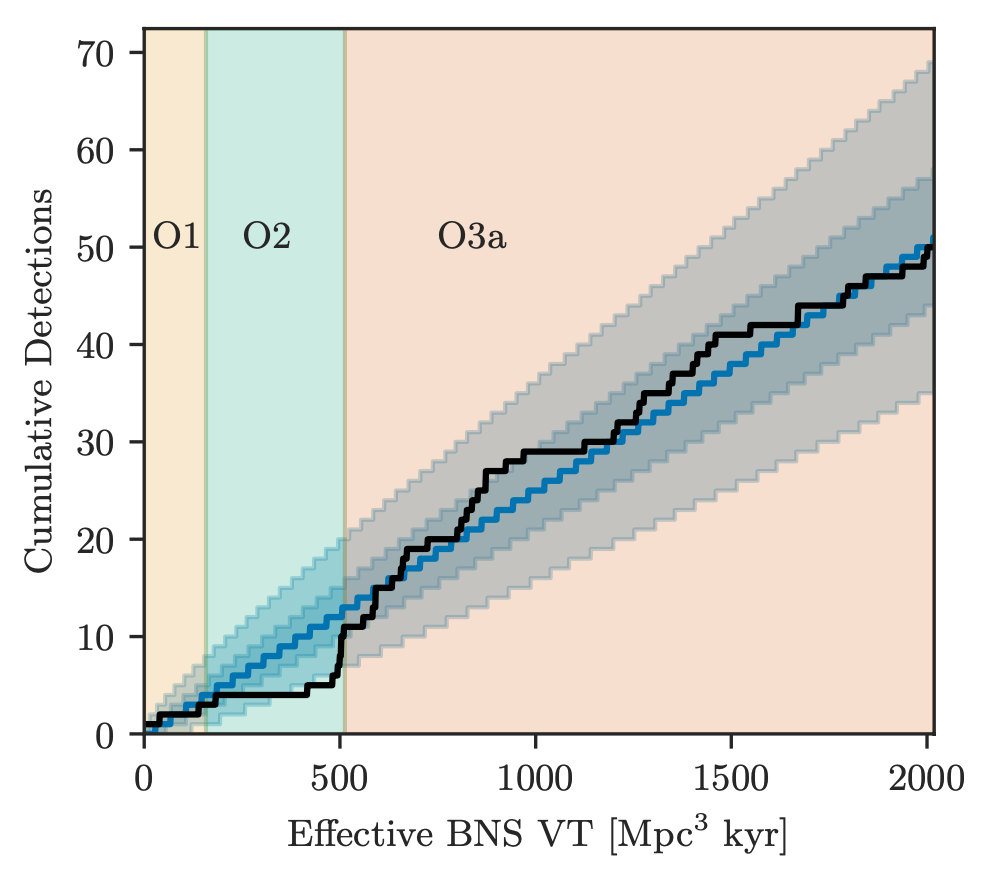
\includegraphics[scale=0.22]{o3detection}
          \centering
          \caption{Cumulative distribution of events and non-retracted alerts of the LIGO-Virgo Collaboration as a function of (observing) time.  The effect of upgrades to the detectors in between runs is clearly visible.  In particular, O3 yielded 56 GW events and alerts: that is 5-times more than those collectively made during O1 and O2. Image credit: LIGO-Virgo Collaboration}. 
          \label{fig:o3detection}
        \end{figure}

        In the remainder of this chapter we will highlight some of the GW observations achieved by the LIGO-Virgo Collaboration and the scientific results connected to them.

\section{The First Observing Run (O1)}

	The first observing run involved the LIGO Hanford Observatory (LHO) and LIGO Livingston Observatory (LLO) detectors, which provided unprecedented sensitivity to GWs
	over a range of frequencies from 30 Hz to several kHz \cite{14}, an interval that  
	covers the frequencies of GWs emitted during 
	the late inspiral, merger, and ringdown of stellar-mass BBHs.

	Two independent matched-filter searches were used to detect GWs from CBC sources: {\ttfamily PyCBC} \cite{109-112} and {\ttfamily GstLAL} \cite{112-114}.
	The pipelines identify GW candidates by looking at coincident events 
	found in both LIGO detectors, in a 15\,ms time window 
	that accounts for the intersite propagation time plus timing uncertainties. 
	Both pipelines used a discrete template bank \cite{42, 114, 115, 117-120}, tartetting binary sources with individual masses from $1{M_\odot}$ to $99{M_\odot}$,
	total mass less than $100{M_\odot}$, and dimensionless non-precessing spins up to 0.99 and 0.05 for BHs and NSs, respectively.

	To assess the candidate significance, they compare the candidate with the noise background, 
	and once an event is confirmed to be a real GW signal, it is removed from the data when estimating the noise background (see Sec.\,$\ref{subsec:far}$).
	Data affected by short duration artifacts of known origin are identified and removed from the analysis dataset.
	After applying this data quality process, the remaining coincident analysis time in O1 was 48.6\,days. 
	The analyses search only stretches of data longer than a minimum duration, 
	to ensure that the detectors are operating stably and enough data is available to build the background noise distribution.  This 
	resulted in 46.1\,days of data for the {\ttfamily PyCBC} analysis and 48.3\,days for the {\ttfamily GstLAL} analysis.

	Three GW events were detected during this run, all three consistent with a BBH source: GW150914, GW151012, and GW151226.
	The binary component masses of all three systems lie 
	within the range expected for stellar-mass BHs. 

\subsection{GW150914: the Birth of Gravitational-Wave Astronomy}

		\begin{figure}[!t]
                	\label{firstgw}
                	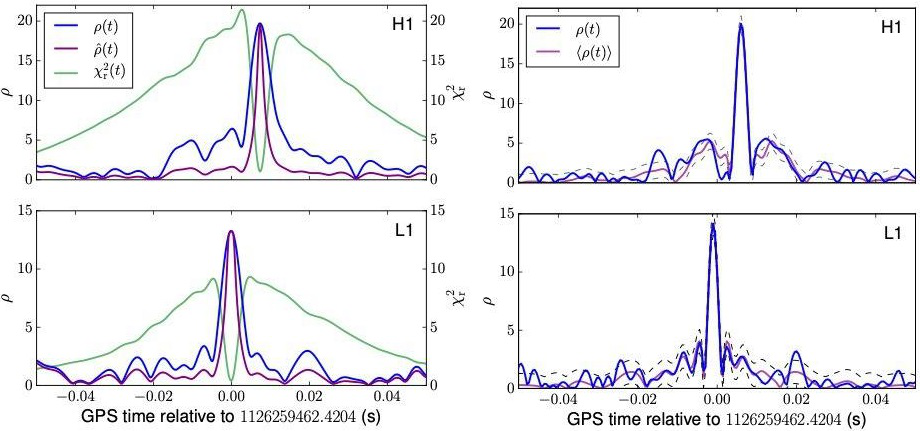
\includegraphics[scale=0.45]{firstgw}
                	\centering
                	\caption{Left: {\ttfamily PyCBC} matched-filter SNR (blue), re-weighted SNR (purple) and chi-squared (green) versus time for the best-matching template at the time of GW150914. The top and bottom plots refer to the Hanford and Livingston detectors, respectively. Right: Observed matched-filter SNR (blue) and expected matched-filter SNR (purple) versus time for the best-matching template at the time of GW150914, as reported by the {\ttfamily GstLAL} analysis. The expected matched-filter SNR is based on the autocorrelation of the best-matching template. The dashed black lines indicate 1-$\sigma$ deviations expected in Gaussian noise. \cite{21}} 
                	\label{fig:firstgw}
                \end{figure}

	The era of GW astronomy began with the detection of the coalescence of two stellar-mass BHs
	on September 14, 2015 at 09:50:45 UTC.  The signal GW150914 was detected with a matched-filter network SNR of 23.7 \cite{21}. 
	Both {\ttfamily PyCBC} and {\ttfamily GstLAL} identified GW150914 as the most significant event in O1 and the probability that 
	it was due to a random coincidence of detector noise is extremely small: 
	both pipelines found no background events with significance 
	equal to or greater than GW150914.  Therefore only an upper limit on the FAR of GW150914 was determined: $6.0 \times 10^{-7}\,$yr$^{-1}$. 
	This corresponds to a $p$-value of $7.5\times10^{-8}$, or a Gaussian-equivalent significance of $5.3\sigma$.  In Fig.\,\ref{fig:firstgw}, taken from \cite{21}, we show a snapshot of the {\ttfamily PyCBC} (left) and {\ttfamily GstLAL} (right) analyses around the time of GW150914.  The SNR timeseries (blue) and reweighted SNR (purple) timeseries otained with the best-matching template peak at time of GW150914, while the normalized chi-squared (green) dips suddenly; this behaviour is observed at both detectors (Handford top, and Livingston bottom).  A similar behaviour holds for the {\ttfamily GstLAL} data that shows the SNR (blue) and expected SNR (purple) timeseries for the same best-matching template.  The two timeseries vary consistently with one another, within the 1-$\sigma$ deviations reported by the black dashed line.

	\subsubsection{Masses}
	The physical parameters of the source of GW150914 were inferred using two waveform models, a non-precessing effective-one-body waveform model (EOBNR) \cite{103, 104} 
	and a precessing spin model (IMRPhenom) \cite{105-107}. 
	Results from the two waveforms are consistent, and match the expectations for a coherent signal of astrophysical origin in both detectors. 
	The total mass of GW150914 was found to be $M^{\rm source} = 65.3^{+4.1}_{-3.4}M_\odot$, with individual masses of $36^{+5}_{-4}M_\odot$ and $29^{+4}_{-4}M_\odot$ \cite{21,41,51}.  This makes the source compatible with a near-equal mass BBH system.
	Following the inspiral, a BBH merges to form a BH remnant; in the case of this signal, the mass of the remnant was $M^{\rm source}_f = 62.3^{+3.7}_{-3.1}M_\odot$.
	The $\sim 3M_\odot$ of difference between $M^{\rm source}$ and $M^{\rm source}_f$ are radiated away in GWs.  While predominantly determined by the total mass, the radiated energy also depends upon the mass ratio and component spins.

	\subsubsection{Spins}
	The results obtained for GW150914 are consistent with expectations for moderately spinning BHs \cite{101, 102}. 
	For equal mass binaries, both components of the spin, 
	parallel and orthogonal to the orbital angular momentum, 
	play a role in the dynamics, but, as the mass ratio tends to zero, 
	the effects of the secondary spin become negligible.
	The spin of the remnant BH, as its mass, is calculated using fitting formulas calibrated against numerical relativity simulations.  It was inferred to be $0.69^{+0.05}_{-0.04}$, as expected for near equal-mass BBH mergers for which the final spin is dominated by the orbital angular momentum of the binary at merger \cite{99, 100}.

	\subsubsection{Distance, Inclination, and Sky Location}
	The signal amplitude is inversely proportional to the luminosity distance to the source: 
	GW150914 has an estimated distance of $D_L = 440^{+150}_{-170}\,$Mpc (redshift $z=0.09^{+0.03}_{-0.03}$). 

	The significant fractional uncertainty for the distance is due to the degeneracy between the distance and the binary inclination with respect to the observer, which both impact the signal amplitude \cite{96-98}.
	The configurations for which the orientation of the binary produces the greatest GW amplitude 
	are either face-on or face-off (angular momentum pointed parallel or antiparallel to the line of sight). 
	The inclination could potentially be better constrained in a precessing system \cite{94, 95}. 
	For GW150914, the data provides a greater posterior support for the source being face-off \cite{93}.

	Sky localization from a GW detector network is primarily determined by the measured delay in the signal arrival times at the sites, 
	with additional information coming from the signal amplitude and phase \cite{91,12}. 
	The arrival time at Hanford relative to Livingstone was $\Delta t_{HL} = 7.0^{+0.02}_{-0.02}$\,s.
	The 90\% credible region for the sky localtion of the source of GW150914 had an area of $230\,$deg$^2$.
	The sky area scales inversely with the square of the SNR \cite{89,90}, 
	and this trend is followed as this event had the smallest sky localisation and 
	highest SNR amongst the events detected during O1.

	\subsubsection{Astrophysical implications}
	This GW discovery provides the first robust confirmation of several theoretical predictions, beyond the existence of GWs:
	heavy BHs exist, BBHs form in nature, and BBHs merge within the age of the Universe at a detectable rate. 
	However, it was impossible to determine the formation channel for this event. 
	Possible BBH formation channels include dynamical formation in a dense stellar environment \cite{84, 88} 
	possibly assisted by gas drag in galactic nuclear disks \cite{82, 83}, or isolated binary evolution, 
	either the classical variant via a common-envelope phase \cite{76-81}, 
	potentially from population III binaries \cite{74, 75}, or chemically homogeneous evolution 
	in close tidally locked binaries \cite{72, 73}. 
	All of these channels have been shown to be consistent with the GW150914 discovery \cite{63-70}. 

        \begin{figure}[!t]
          \label{o1}
          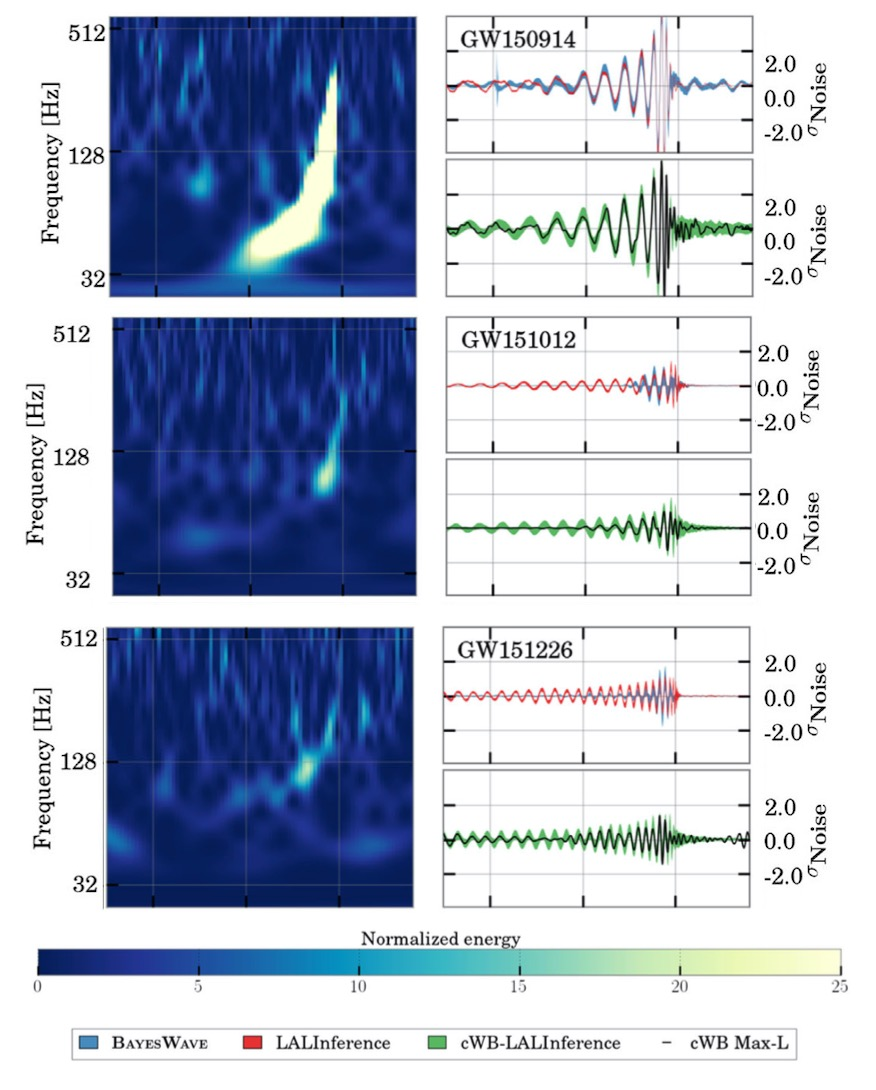
\includegraphics[scale=0.4]{o1}
          \centering
          \caption{Time-frequency maps and reconstructed signal waveforms for the three O1 BBH events. Each row refers to a single event.  The three panels in a row show whitened data from the LIGO detector where the higher SNR was recorded. The panel on the left is a normalized time-frequency power map of the GW strain.  The two panels on the right show time-domain reconstructions of the whitened signal, in units of the standard deviation of the noise. The upper panel shows the 90\% credible intervals from the posterior probability density functions of the waveform timeseries inferred by a Bayesian pipeline that used the PhenomP waveform templates ({\ttfamily LALInference}, red band) and by a pipeline that used wavelet reconstruction ({\ttfamily BayesWave}, blue band).  The lower panel shows the maximum likelihood point estimate from the {\ttfamily cohrent WaveBurst} unmodelled search (solid lines), along with a 90\% confidence interval (green band) derived from the {\ttfamily cohrent WaveBurst} analyses of simulated waveforms generated starting from the {\ttfamily LALInference} posterior and injected into data near each event. \cite{13}}
          \label{fig:o1}
        \end{figure}


\subsection{GW151012 and GW151226}

Two more GW signals were detected during O1, and both were consistent with a BBH source: GW151012 and GW151226.  A summary of all three observations is provided in Fig.\,\ref{fig:o1} \cite{13}.  This shows the time-frequency maps and reconstructed waveforms for all three O1 events.

	GW151012 is the third most significant GW event from O1.  It was first referred to as LVT151012, where LVT stands for LIGO-Virgo Transient: this was due to the fact that it
	was originally detected with a low statistical significance of $1.7\sigma$, 
	corresponding to a FAR of one in 2.7 years.  The trigger was later reanlyzed with improved O2 versions of the pipelines and its significance was increased: the signal now meets the criteria of a confident detection of a BBH merger, and was therefore re-labeled as GW151012.  The final values of the network SNR for this signal are 9.5 and 10.0 for the {\ttfamily PyCBC} and {\ttfamily GstLAL} pipelines, respectively \cite{13}.

	GW151226 was the second observation of a coincident GW signal to be announced. 
	Its combined matched-filter SNR was 13. 
	The signal was identified as the second most significant event by both the {\ttfamily PyCBC} and {\ttfamily GstLAL} analyses.
	GW151226 was more significant than all O1 background events in the {\ttfamily PyCBC} analysis, 
	after having removed any background events associated with GW150914 from the distribution.
	Its FAR has an upper limit of $6.0 \times 10^{-7} yr^{-1}$, which
        corresponds to a $p$-value of $< 7.5 \times 10^{-8}$, or a Gaussian-equivalent significance of at least $5.3\sigma$. 
	In the {\ttfamily GstLAL} analysis, the background extends past the observed log-likelihood of GW151226, 
	and the event is recovered with a FAR of 1 per 44000 years, which corresponds to a $p$-value of $3.5\times 10^{-6}$ and a significance of $4.5\sigma$.

	GW151226 persisted in the LIGO frequency band for approximately 1\,s, 
	increasing in frequency and amplitude over about 55 cycles from 35 to 450\,Hz. 
	This differs from the more massive GW150914 binary for which only the last 10 cycles of the inspiral where observable.  This has an immediate effect on the precision with which the chirp mass \cite{126, 127} recovered with respect to the case of GW150914, as this physical parameter controls the binary evolution during the early inspiral.  \fpg{Qui allora dovresti riportare le due chirp masses per fare un confronto.}

	The source of GW151226 was an unequal-mass system with two stellar-mass BHs 
	with a source-frame masses of $m_1 = 13.7^{+8.8}_{-3.2}M_\odot$ and secondary mass $m_2 = 7.7^{+2.2}_{-2.5}M_\odot$ \cite{13}. \fpg{Stavi citando i valori del paper originale, questi sono quelli finali del catalog visto che giustamente parli di GW151012 e non pi\`u di LVT151012, ovvero tieni conto delle rianalisi.} 
	The inferred BH masses are within the range of dynamically measured masses of BHs found in X-ray binaries \cite{128-132}, unlike the high masses of GW150914 which had never been observed before. Finally,
        the two LIGO detectors are nearly coaligned and the source of GW151226 is likely to be located close to the maxima of the directional responses of both detectors \cite{28}. 
	Consequently, it is difficult to extract the polarization content, and therefore the orientation of the orbital plane. 
	As a result, the luminosity distance is only weakly constrained to be $D_L = 450^{+180}_{-190}Mpc$, which is comparable to the one of GW150914 and corresponds to a redshift of $0.09^{+0.04}_{-0.04}$.


\section{The Second Observing Run (O2)}

	Between O1 and O2 run the sensitivity of both LIGO instruments was improved and 
	at LLO further improvements were made during O2. 
	As a result, the LLO BNS range --- i.e., the distance, averaged over sky position and inclination, up to which a binary made by two $1.4M_\odot$ NSs is detecteble --- increased from about 60\,Mpc to 80\,Mpc at the beginning of O2.  this was later increased by another $\sim 20\%$.
 	Despite its lower BNS range ($\sim 25\,$Mpc) Virgo provided a fundamental contribution in determining the source localization and orientation \cite{56}, as well as in boosting the significance of the events. This was of paramount importance in kick-starting multimessenger astronomy with GWs.
	In addition to the instrument upgrades, developments were also carried out on
	the search algorithms.
 
	Of the eight GW signals detected during O2 (GW170104, GW170608, GW170729, GW170809, GW170814, GW170817, GW170818 and GW170823), the five August events were localized by the three detector LHO, LLO and Virgo (HLV) network.  Additionally, GW170104, GW170814, GW170608, and GW170817 where published, in that order, as single events \cite{60,61,62,138}.   
	In order to quantify the FAR with an accuracy that enabled the claim of confident detections, the O2 data was divided into periods of 5 days of two-detector cumulative coincident observing time.
	This time, the searches targeted  detector-frame total masses from $2M_\odot$ to $500 M_\odot$, whereas the spin target space remained unchanged.
	Since GW151226 is a low mass binary, the chirp  mass is well measured $8.9^{+0.3}_{-0.3} M_\odot$,
	while for the higher mass system GW150914 is $28^{+2}_{-2}M_\odot$.
\subsection{GW170104: a 50-Solar-Mass Binary Black Hole Coalescence}

	The observation of GW170104 was made by the LIGO detectors, 
	with a network SNR of 13 and a FAR of less than 1 in 70,000 years.
	At the detection statistic value of GW170104, the background rate in both matched filter 
	analyses is dwarfed by the signal rate, yielding a probility of astrophysical origin greater than $1 - (3 \times 10^{-5})$ \cite{60}. \fpg{Citazioni.}

	The source of GW170104 is a BBH system with total mass of $\sim 50M_\odot$.  	
	The inferred component masses are $31.2^{+8.4}_{-6.0}M_\odot$ and $19.4^{+5.3} _{-5.9}M_\odot$.
	The BH spins are best constrained through measurement of the effective inspiral spin parameter, $\chi_{eff}$, 
	a mass-weighted combination of the spin components perpendicular to the orbital plane; the credible interval found was $\chi_{eff} = −0.12^{+0.21}_{−0.30}$. 
	This result implies that the BH spins show a preference for being 
	anti-aligned with the orbital angular momentum, but the zero spin possibility is not excluded. 
	This is distinct from the case for GW151226, which had a strong preference 
	for spins with positive projections along the orbital angular momentum \cite{58}.
	Finally, the source luminosity distance is $880^{+450}_{−390} Mpc$ corresponding to a redshift of $z = 0.18^{+0.08}_{−0.07}$. 

	The high source mass values suggest formation in a sub-solar metallicity environment \cite{134, 134}, which weakens the stellar winds that cause mass loss during the lifetime of the progenitor stars.
	The inferred merger rate agrees with previous calculations \cite{59, 137}, and could potentially be explained 	
	by BBHs forming through isolated binary evolution or dynamical interactions in dense stellar clusters \cite{134}. 

\subsection{GW170608}

	GW170608 was first identified as a loud (SNR $\sim9$) event in LLO data,
	via low-latency templated searches \cite{138}.	
	The morphology of the LLO event is consistent with a CBC signal, 
	but a noise origin could not be ruled out using LLO data alone. 
	Consequently, LHO data were investigated and were determined to be stable 
	at frequencies above 30Hz, which was established as the starting frequecy to look into a segment of LHO data around the event time.
	{\ttfamily PyCBC} and {\ttfamily GstLAL} then identified GW170608 with a network SNR of 13,
	and a FAR of less than 1 in 3,000 years and 1 in 160,000 years, respectively.

	The binary source of GW170608 consisted of two compact objects with source-frame component masses 
	$12^{+7}_{-2}M_\odot$ and $7^{+2}_{-2}M_\odot$.  
	Since NSs are expected to have masses below $\sim 4M_\odot$ \cite{141},
	both objects are most likely BHs. 
	The $\chi_{eff}$ inferred from this event is $0.07^{+0.23}_{−0.09}$,
	disfavoring large, anti-aligned spins on both BH.
        Finally, GW170608 was localized at a luminosity distance of $D_L = 340^{+140}_{−140}Mpc$, and within a sky area of $\sim 520\,$deg$^2$, determined largely by the signal's measured arrival time at LLO $\sim 7$\,ms later than at LHO.
 
	The inferred component masses of GW170608 are consistent with dynamically-measured masses of BHs found in low-mass X-ray binaries.
	The low masses involved imply that this time a high-metallicity progenitor environment is possible, as this causes significant mass losses from the progenitor stars via strong stellar winds \cite{142}.
	However, formation at lower metallicity with comparatively lower mass progenitors is not excluded.

\subsection{GW170814: the First Three-Detector Network Observation}	

	On August 14, 2017, a GW signal coming from the merger of two stellar mass BHs 
	was observed for the first time by a three detector network, comprised of the Virgo and two LIGO detectors. 
	GW170814 was first identified with high confidence by two independent 
	low-latency matched-filter pipelines \cite{111,143,144,145,146,149},
	with a Hanford-Livingston network SNR of 15 and a three-detector network SNR of 18 \cite{114,150,151}.
	The improvement in significance achieved by including Virgo data in the analysis is particularly evident for this event: when data from all thee detectors is used, the FAR of the event is $< 1$ in 5,900 years, while the LIGO-only FAR is approximately 1 in 300 years.

	The component masses of the source inferred through a coherent Bayesian analysis \cite{93, 152} 
	of offline noise-subtracted data for the LIGO and Virgo detectors 
        are $30.5^{+5.7}_{-3.0}M_\odot$ and $25.3^{+2.8}_{-4.2}M_\odot$.
	For events detected by the two LIGO instruments alone, the localisation was often limited to roughly annular regions by the baseline formed by the two LIGO detectors,
	spanning hundreds to about a thousand square degrees at the 90\% credible level \cite{165-167}. 
	The inclusion of Virgo contributes with additional independent baselines, 
	which for GW170814 and similar events can reduce the positional uncertainty by an order of magnitude or more \cite{166}. 
	For an initial rapid localization performed with LHO and LLO data, 
	the 90\% credible area on the sky was $1160\,$deg$^2$: the inclusion of Virgo shrunk this down to $100\,$deg$^2$.
	Incorporating Virgo data also reduces the uncertainty on luminosity distance, which goes from $570^{+300}_{-200}\,$Mpc (two-detector rapid localization) to $540^{+130}_{-210}\,$Mpc (full network).

	 Since the two LIGO instruments have similar orientations, the information about polarization is minimal when the LIGO instruments alone.  Virgo data
	allowed to investigate GW polarizations for the first time, by geometrically 
	projecting the wave amplitude onto the three detectors.
	Generic metric theories predict that any combination of tensor, vector, or scalar 
	polarizations \cite{171,172} can characterize metric perturbations.
	So far, some evidence that GWs are described by the tensor (spin-2) metric perturbations 
	of general relativity has been obtained from measurements of the orbital decay rate of binary pulsars \cite{173,176}, 
	and from the GW phase evolution of BBH mergers observed by LIGO, in the framework of parametrized models \cite{52,57,60}. 
	The results of the analysis of GW170814 with Virgo data show that the data strongly favor
	pure the tensor polarizations of general relativity, over pure scalar or pure vector polarizations.

        \begin{figure}[!t]
          \label{o2}
          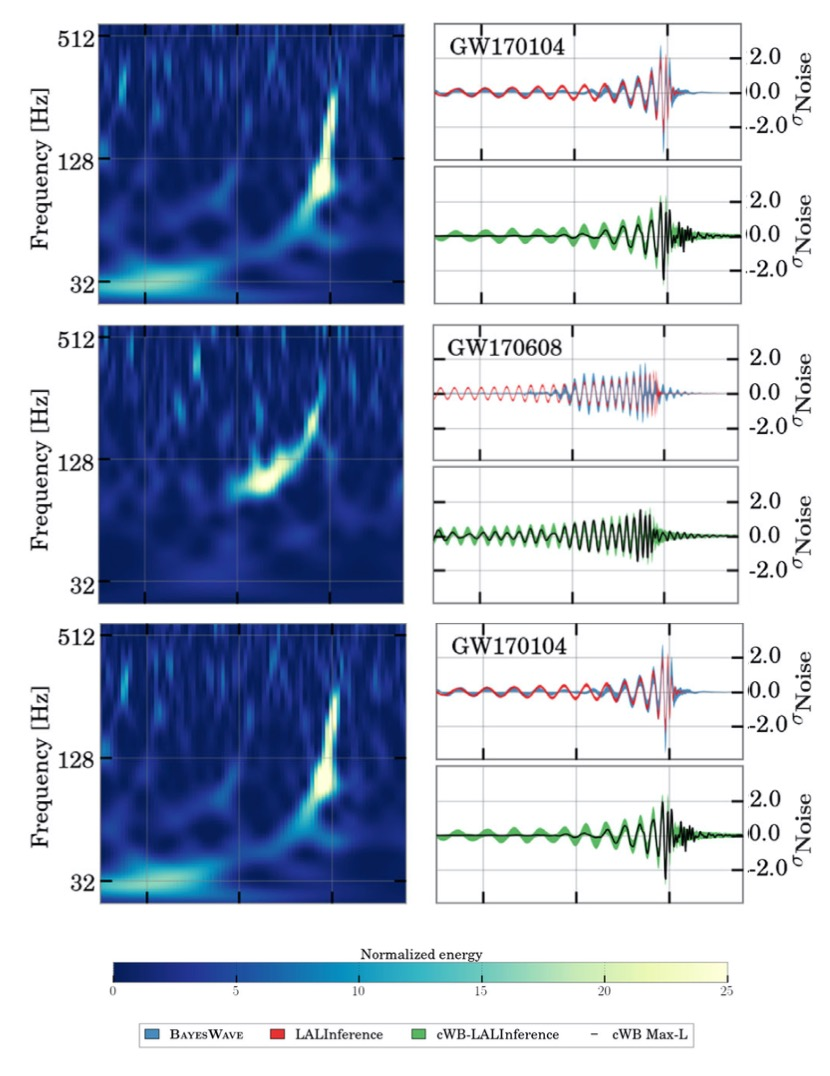
\includegraphics[scale=0.45]{o2}
          \centering
          \caption{Same as Fig.\,\ref{fig:o1} but for the O2 events: GW170104, GW170608 and GW170814.}
          \label{fig:o2}
        \end{figure}

\subsection{GW170817: the Birth of Multimessenger Astronomy}

	On 17 August 2017 the first GW signal compatible with a BNS source was detected by the LIGO-Virgo Collaboration.  The GW170817 candidate was first registered in low latency \cite{112,114}
	as a single-detector trigger in LHO data. 
	An offline re-analysis \cite{28,111} of data from the whole LIGO-Virgo network 
	confirmed the presence of a significant coincident signal with a combined SNR of 32.4.
	The offline analysis then identified the FAR of GW170817 to be less than 1 in 80,000 years \cite{61}. 
	The source was localised \cite{59,152} in a region of $28\,$deg$^2$ at a distance of $40^{+8}_{-14}$ Mpc, 
	consistently with the early estimates disseminated through GCN Circulars \cite{55,60}.
	The inspiral stage of the binary coalescence dominates 
	the portion of GW170817 in the detector sensitivity bands, 
	and as a consequence, the chirp mass, which drives the frequency evolution of gravitational radiation at the leading order, 
	is the best constrained parameter with a value of $1.188^{+0.004}_{-0.002}M_\odot$.
	The measured component masses are in the range $0.86$--$2.26M_\odot$
	consistent with a compact binary with two NSs.

        In of itself this observation already constitutes a remarkable result, but more historical results poured in that day and in the following months.  $\sim1.74$\,s after the trigger time of GW170817, the {\it Fermi}/GBM and INTEGRAL SPI-ACS instruments recorded GRB 170817A \cite{147, 140} which was shown to be unambiguously associated with the source of GW170817 \cite{55}.  This was the first
        confident joint GW and electromagnetic observation in history (see Fig.\,\ref{fig:gw-grb}).
	Standard follow-up analyses \cite{108,110} of the {\it Fermi}/GBM trigger 
	determined the burst duration to be $T_{90} = (2.0 \pm 0.5)\,$s,
	therefore GRB 170817A was classified as a short GRB, with 3:1 odds over being a long GRB.
        The classification is further supported by incorporating 
	the hardness ratio of the burst and comparing it to the {\it Fermi}/GBM catalog \cite{110}.  The unambigious association of GW170818 and short GRB 170817A confirmed that BNSs can be the progenitors of short GRBs, a question that had remained open for decades in high-energy astrophysics.

        Having received notice of the observation of short GRB 170817A by {\it Fermi}, the LIGO-Virgo Collaboration ran
        two offline targeted {\it coherent} searches on its data, as it does for all {\it Fermi} and {\it Swift} GRB observations.  The first targeted search ({\ttfamily PyGRB} \cite{111,116,213}
	looks for subthreshold GW signals in the data by searching for BNS and NS–BH binary merger signals compatible with the time and sky-location of short GRBs.  This search is carried out in a $[-5, +1]\,$s window around the GRB trigger time \cite{55}. 
	This search recovered GW170817, as expected, with a $p$-value of $<9.4\time 10^{-6}(>4.2\sigma)$: this significance estimate is limited by computational resources used to estimate the noise background. 
	The second coherent search does not assume any particular GW morphology or GRB model 
	\cite{55,144,145} and it allows for a $[-600, +60]\,$s search window,
	in order to address potentially higher time-of-arrival separations 
	that may arise for long GRB triggers.
	This unmodelled search also recovered GW170817, with a $p$-value of $1.3\times 10^{-5} (4.2\sigma)$.

	The observation with excellent localization of GW170817 triggered a huge electromagnetic follow-up campaign \cite{194} which produced observations across the whole electromagnetic spectrum.
	This captured an infrared transient (kilonova), which allowed for the identification of the host galaxy of the source 
	and is associated with the aftermath of the BNS merger.
	Delayed X-ray and radio counterparts that provide information on the environment of the binary where also registered.
        
        \begin{figure}[!t]
          \label{gw-grb}
          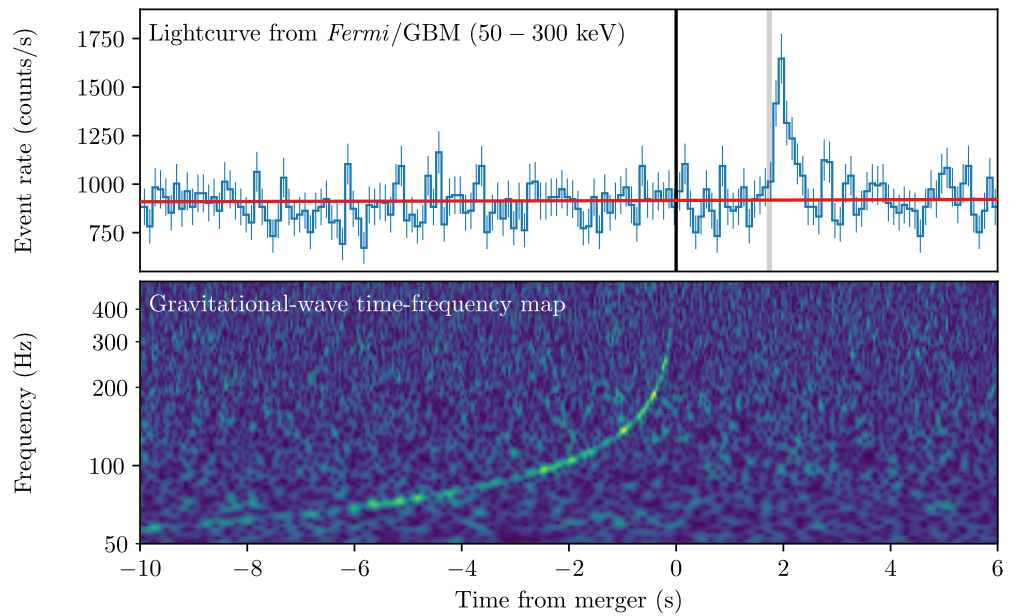
\includegraphics[scale=0.45]{gw-grb}
          \centering
          \caption{Joint, multi-messenger detection of GW170817 and GRB 170817A. Top: the GBM lightcurve in the 50--300\,keV energy range. The background estimate from \cite{110} is overlaid in red. Bottom: the time-frequency map of GW170817  obtained by coherently combining LHO and LLO data. All times here are relative to the GW170817 trigger time. \cite{55}}
          \label{fig:gw-grb}
        \end{figure}


\section{The Third Observing Run (O3)}

	Between O2 and O3, several improvements were made to increase the detector sensitivities.  For the LIGO detectors, 
	the input laser power was increased, a squeezed vacuum source 
	at the interferometer output was added and noise arising from scattered light was mitigated.  
	Additionally, end test-mass optics with lower-loss coatings, along with new reaction masses, 
	were installed in each interferometer \cite{53}. 
	The BNS inspiral range reached $102$--$111\,$Mpc for LHO and $125$--$140\,$Mpc for LLO during the first part of O3.
	Virgo doubled its sensitivity compared to O2, thanks to a series of improvements: 
	fused silica fibers were installed as a replacement of the steel test-mass suspensions, technical noises were reduced, the input laser power was increased 
	and a squeezed vacuum source was installed. 
	This brought the Virgo BNS inspiral range to $43$-–$50\,$Mpc over the first three months of O3, as shown in Fig.\,\ref{fig:o3bnsrange}. 
	These improvements successfully impacted the detection rate (Fig.\,\ref{fig:o3detection}).  In spite of the early suspension of O3, 
	56 public alerts were sent and non-retracted and of these four have already been published as special events: GW190412, GW190425, GW190521, and GW190814.
        
        \begin{figure}[!t]
          \label{o3bnsrange}
          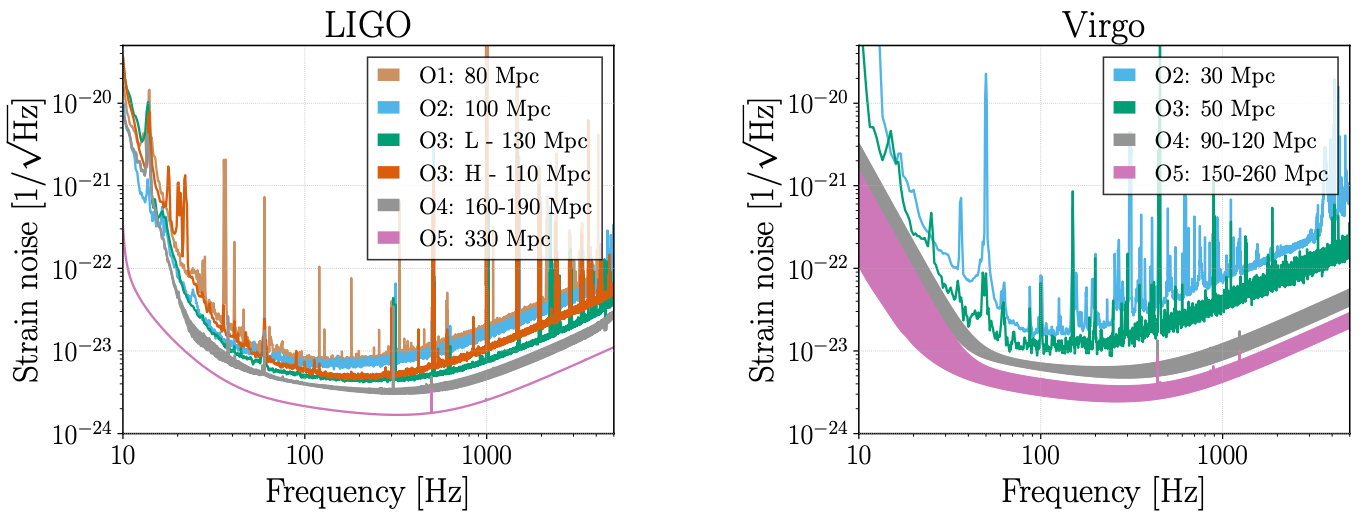
\includegraphics[scale=0.5]{o3bnsrange}
          \centering
          \caption{Advanced LIGO (top left), Advance Virgo (top right) target strain sensitivities as a function of frequency. The quoted range is for a $1.4M_\odot + 1.4M_\odot$ BNS merger.  The BNS range (in Mpc) achieved in past observing runs and anticipated for future runs is shown.  The O1 LIGO curve is taken from the LHO, while the O2 one comes from LLO; in both cases they refer to the interferometer with better performance for the observing run in question. The O3 curves reflect recent performance. For future runs the anticipated ranges are shown as bands reflecting the uncertainty in the impact of improvements and upgrades to the overall sensitivity. \cite{53}}
          \label{fig:o3bnsrange}
        \end{figure}

\subsection{GW190412: a Binary-Black-Hole with Asymmetric Masses}
	GW190412 is a loud event detected with by the LIGO-Virgo three detector network with network SNR of 19 and a FAR of 1 in 30,000\,yrs.
	The peculiarity of this event is the asymmetry in the binary component masses:
	one is a $\sim 8M_\odot$ BH, while its companion has a mass of $\sim 30M_\odot$.
	While the individual masses of the BBH were consistent with whose of preious GW events,
	the mass ratio is unlike any of the other BH mergers detected before. 
	This allows to observe a fundamental property of GWs.

	In general relativity, gravitational radiation
	is observed as a combination of two polarizations, weighted with the detector response functions, see Eq.\,(\ref{beampattern}). 
	This quantity can be expressed also as $h = h_{+}-ih_{\times}$ and expanded into multipole moments 
	using spherical polar coordinates defined in a source centered frame \cite{225}
        \begin{equation}
          h_{+}-ih_{\times} = \sum_{l \geq 2} \sum_{-l \leq m \leq l} {{h_{lm}(t, \boldsymbol{\lambda})} \over {D_L}} _{-2} Y_{lm}(\theta, \phi)
        \end{equation}
	The radiative multipoles, $h_{lm}$, depend on the source properties, while the source geometry 
	depends on mass ratio and is most prominently manifested in the relative contribution 
	of multipoles with odd or even azimuthal index, $m$.
	For an exactly equal mass binary with non-spinning components, only multipoles with even $m$ 
	respect orbital symmetry and so are present in the radiation \cite{187}, resulting in the quadrupole, $h_{22}$, 
	being the most dominant, followed by other multipoles with even $m$. 
	Otherwise, for sufficiently unequal mass ratios, the $l = m = 3$ and subsequent 
	multipoles with $l = m$ gain increasing importance \cite{187-192}.
	GWs of higher harmonics had not been observed until GW190412:
	these higher multipoles makes a significant, measurable contribution to the observed data as shown in \cite{133}.

	As a result of the richer detectable multipole content, the orientation of the binary is more accurately determined and 
	tighter bounds are obtained on intrinsic source parameters, such as the mass ratio and primary spin magnitude, 
	which constitutes the tightest constraint on the individual spin magnitude of a BH obtained with GWs so far. 
	Even though the $\chi_{eff}$ is found to be positive, large in-plane spin components are absent, 
	indicating that the system is slightly precessing.
	The degeneracy between luminosity distance and inclination angle that is typical 
	in the results obtained when higher multipoles are suppressed is broken when higher multipoles are visible, 
	resulting in more precise measurements of these parameters.

	The new observation also provides new insight into the BBH merger rate, 
	showing clearly that unequal-mass systems are less likely, but still expected to form in the universe. \cite{133}

        \begin{figure}[!t]
          \label{asymmetric}
          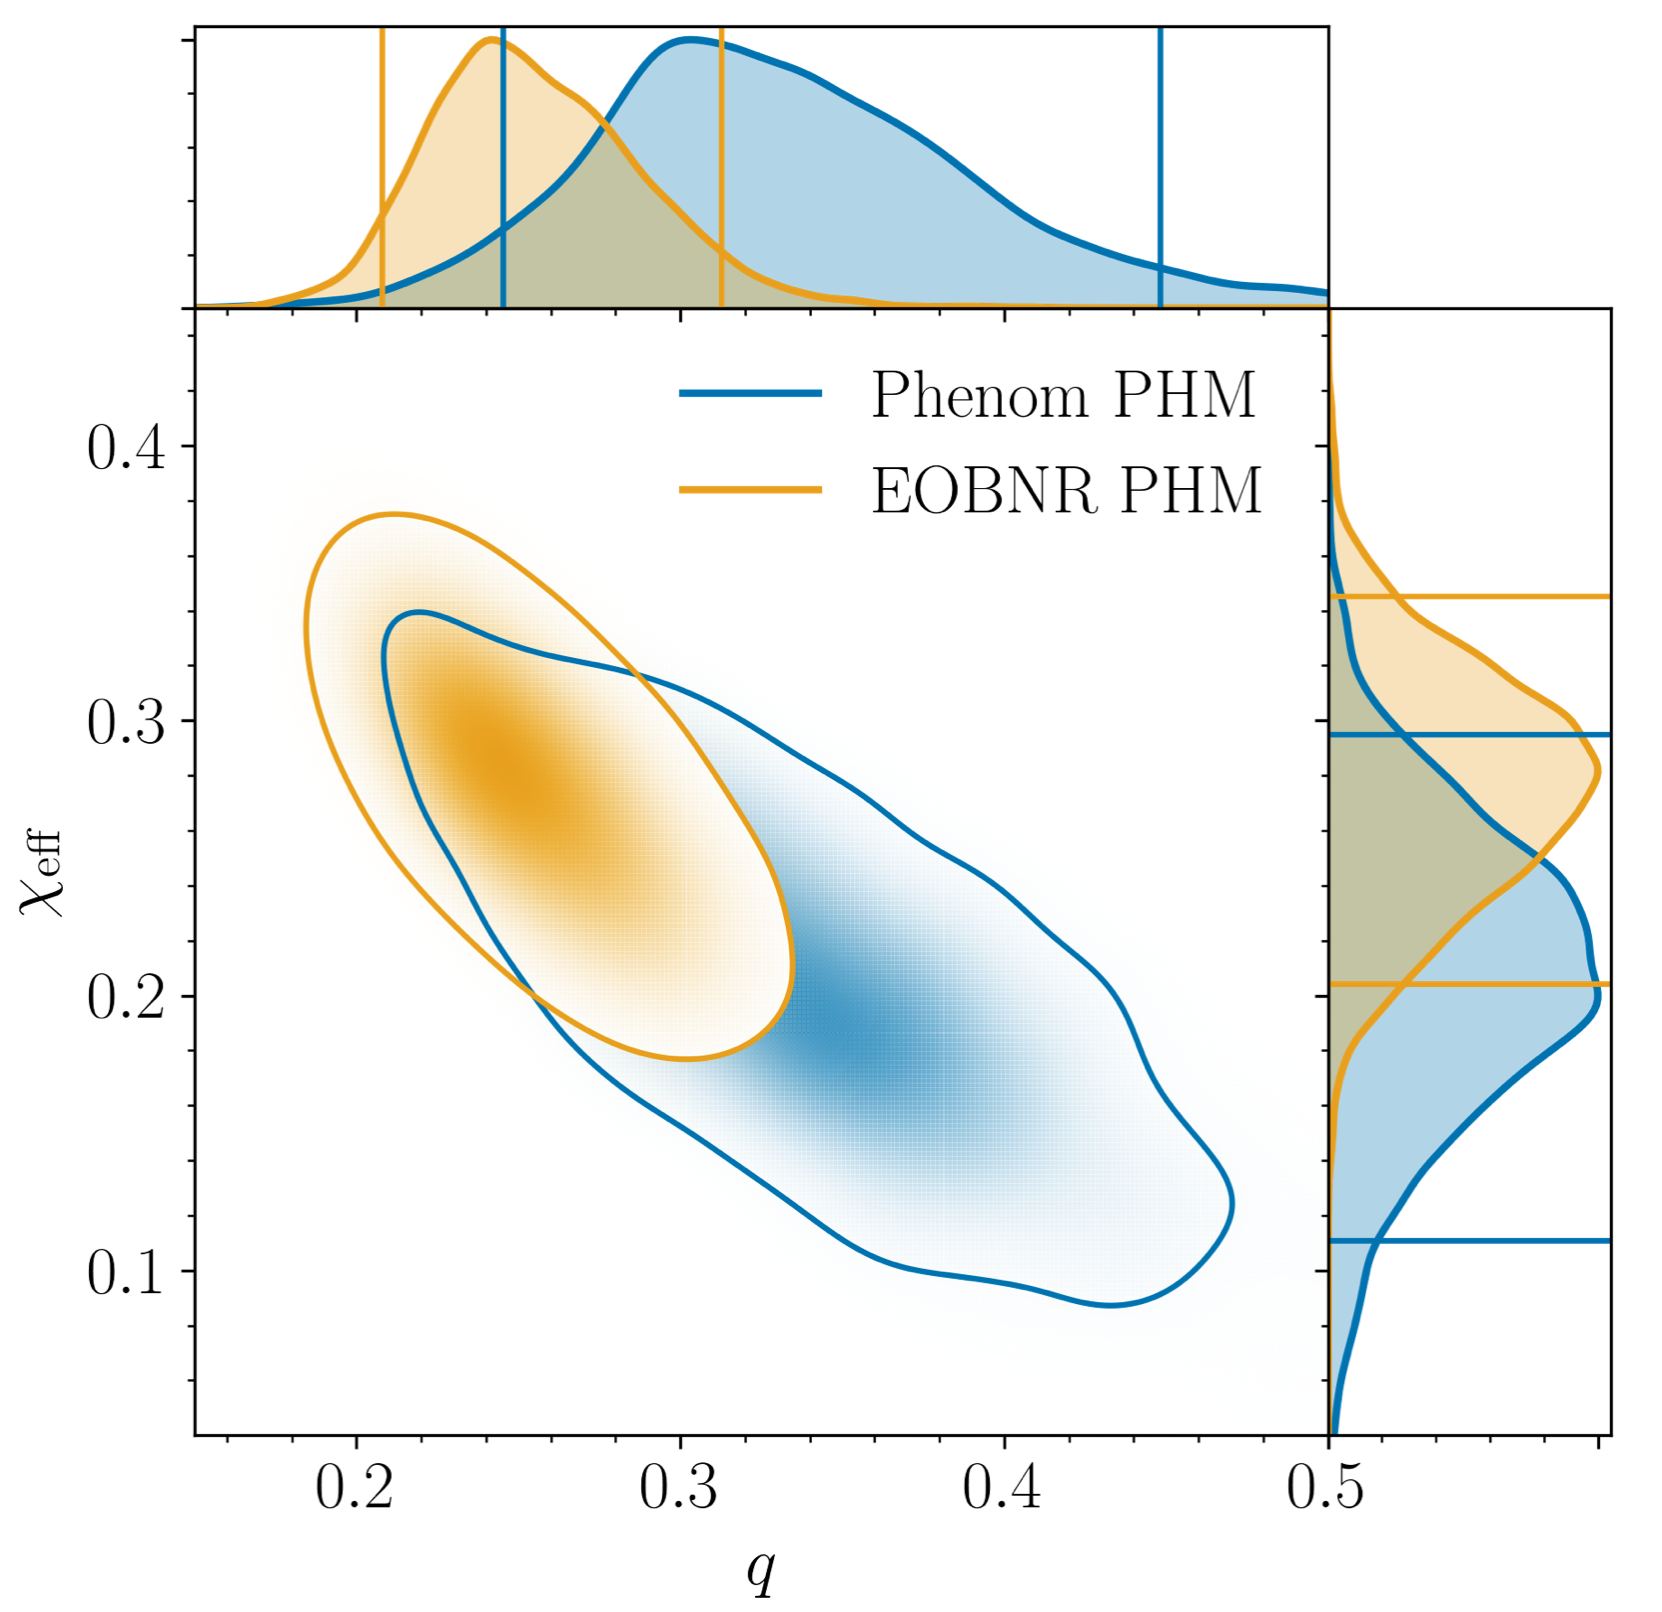
\includegraphics[scale=0.2]{asymmetric}
          \centering
          \caption{The inferred mass ratio $q$ and effective spin $\chi_{eff}$ of GW190412. The distributions reported in orange and blue are obtained with two distinct waveform models. \cite{133}} 
          \label{fig:asymmetric}
        \end{figure}

\subsection{GW190425: a Compact Binary Coalescence with Total Mass $\sim 3.4M_\odot$}

	GW190425, observed by LLO, is the second GW event
	consistent with the inspiral of a BNS system.
	This event was detected in real time processing, with an SNR of 12.9 in LLO; 
	Virgo was operating at the time of the event, but observed the event with an SNR of 2.5, 
	which is below the threshold of 4 at which searches consider triggers for significance estimation. 
	The difference in SNR between LLO and Virgo is consistent with the difference 
	in the sensitivities of the two detectors, considering that LLO had 
	a BNS inspiral range of $\sim 135\,$Mpc, while for Virgo it was $\sim 48\,$Mpc.

	The single detector observation has a couple of consequences. 
	One is that the localization area is the sky is so large
	that it constitutes a significant challenge for follow-up searches for electromagnetic counterparts. 
	The absence of counterparts means that there is no confirmation that the source was indeed a BNS; 
	it is therefore possible that one or both of the merging objects were actually 
	BHs with masses smaller than any BH mass observed so far \cite{148}.
	Secondly, having a single-detector poses a challenge on determining the FAR.
	The low-latency FAR was estimated using data collected in O3 
	up until the time of the event, and it was found to be one in $69,000\,$yrs. 
	To further establish the significance of GW190425, 169.5 
	days of background in the BNS part of the parameter space from O1 and O2 were used in addition to the 50 days  
	from O3.  The event was found to be 
	louder than any background event up to its detection \cite{148}.

	The binary primar component mass is between $1.61M_\odot$ and $2.52 M_\odot$, 
	while the secondary mass falls between $1.12M_\odot$ and $1.68 M_\odot$.
	This event is particularly special because of its total mass of $3.4^{+0.3}_{-0.1} M_\odot$ 
	and chirp mass of $1.44^{+0.02}_{-0.02}M_\odot$, which are are significantly larger 
	than those of any other known galactic BNS system to date. 
	Currently, there are 17 known galactic NS pairs with measured total masses 
	that range from $2.5$ to $2.9M_\odot$.
	Fitting a normal distribution to the total masses of ten galactic BNS systems, 
	which are expected to merge within the lifetime of the Universe, 
	shows that the average galactic binary mass is about $2.69M_\odot$, 
	while the mass of the GW190425 source is about $3.4M_\odot$, that is,
	it is 5 standard deviations away from the Galactic mean, as shown in Fig.\,\ref{fig:secondbns}.

        \begin{figure}[!t]
          \label{secondbns}
          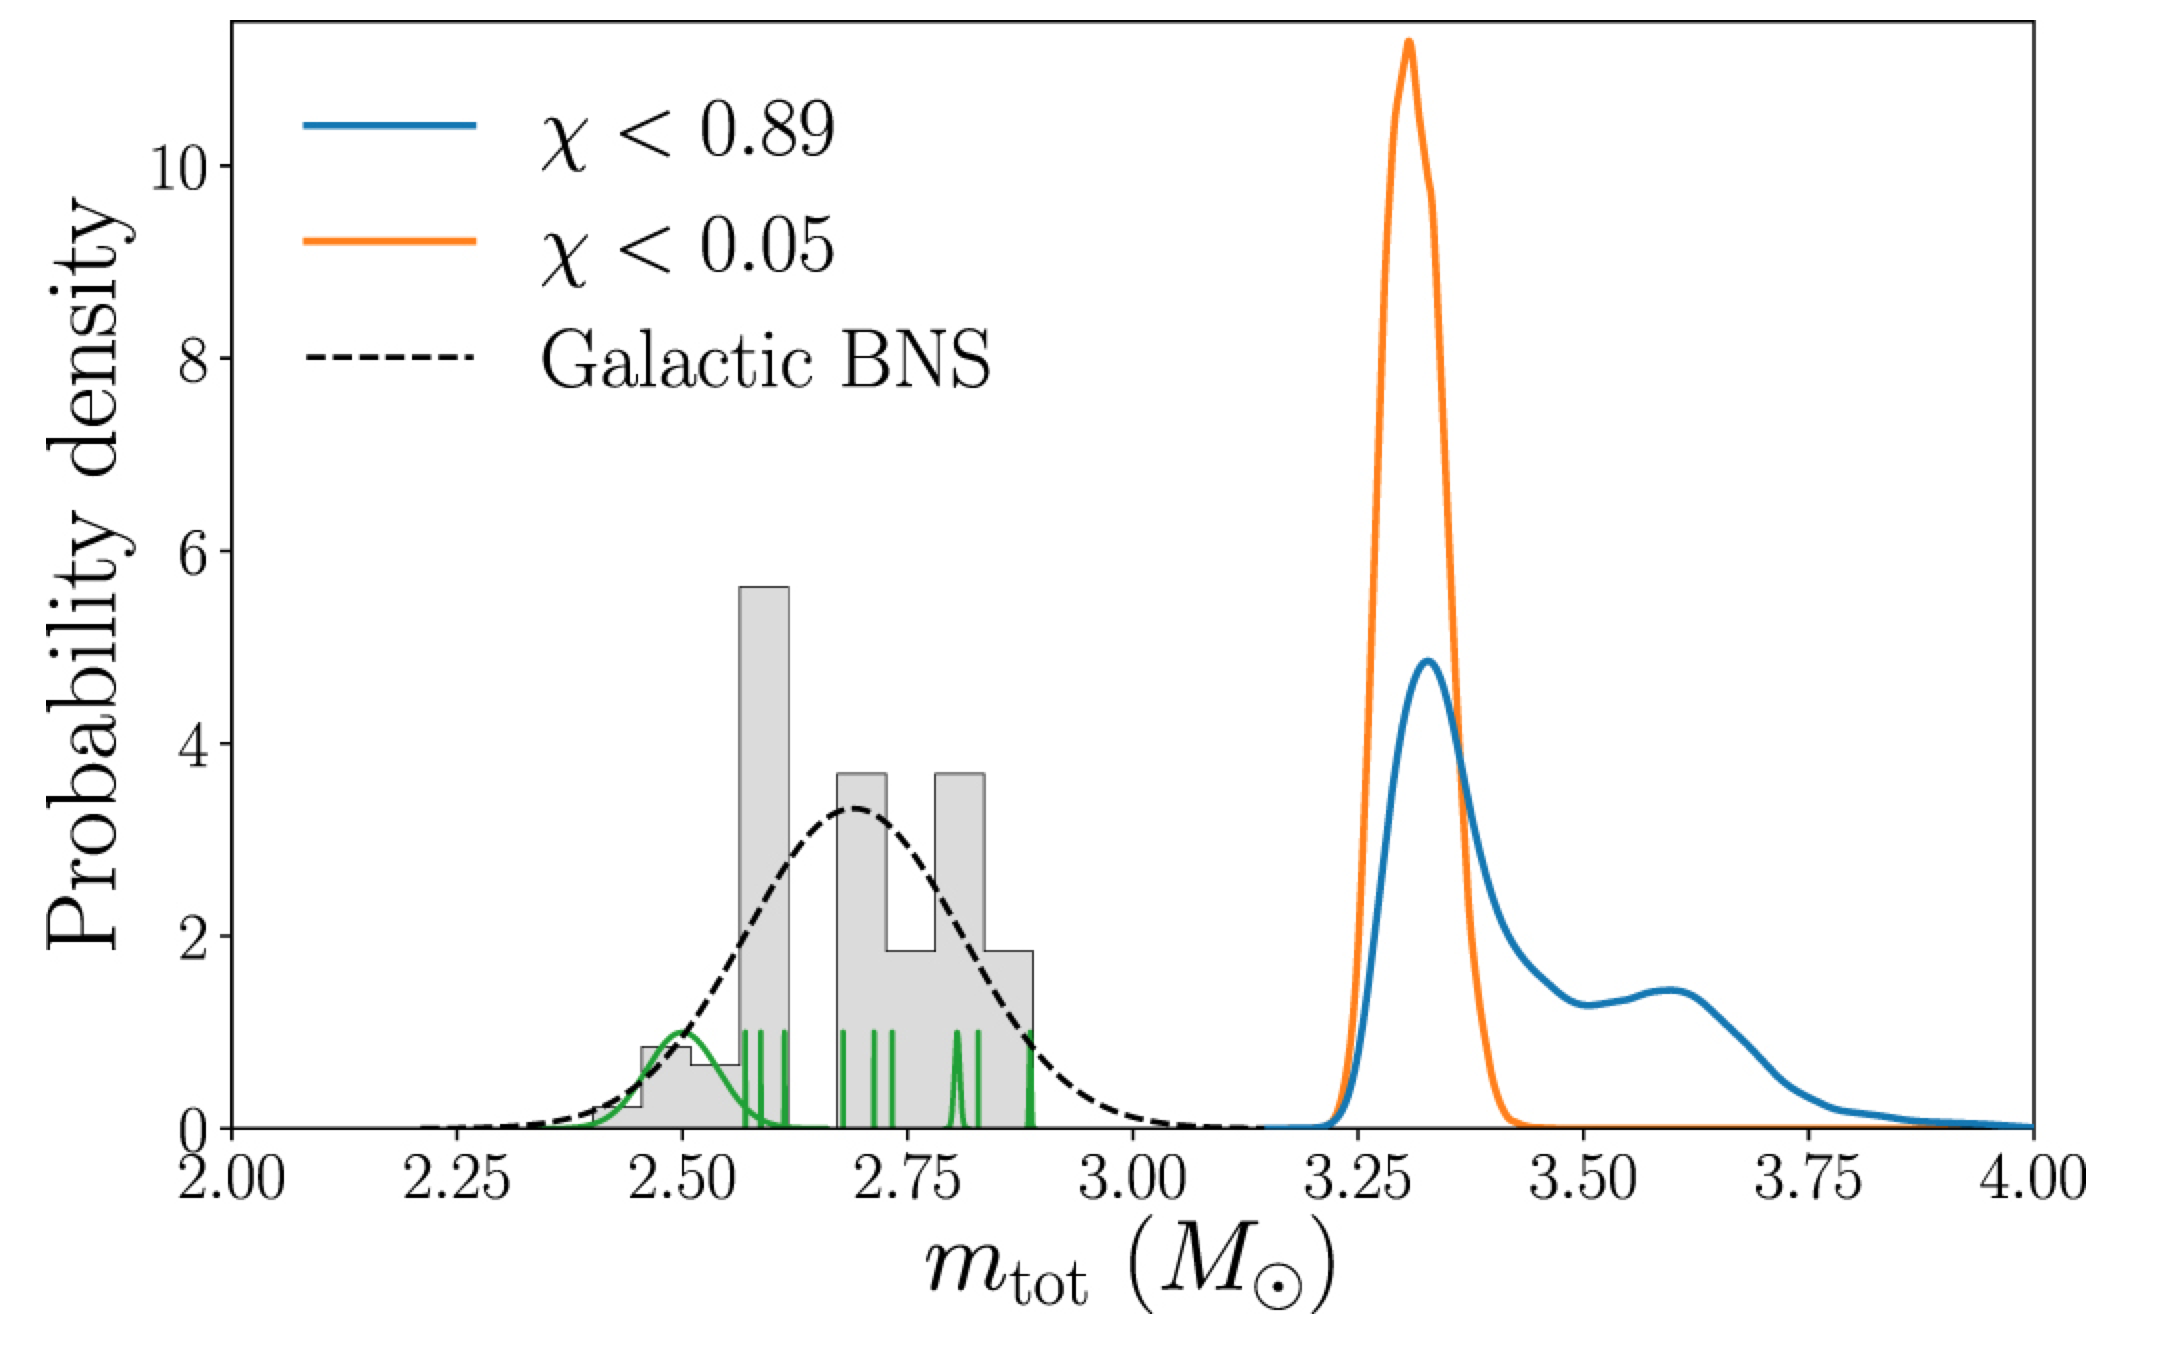
\includegraphics[scale=0.3]{secondbns}
          \centering
          \caption{Blue and orange curves are the total mass posteriors of GW190425 obtained by using different priors for the spins of the two NSs. In both cases, these distributions are dramatically different from the distribution of total masses of known galactic BNSs, reported with the grey histogram and fitted by the black dashed line. \cite{62}}
          \label{fig:secondbns}
        \end{figure}

	The unusual total mass of GW190425 may have implications for the origin of its source \cite{148}.
	There are two ways in which we expect to form BNS. 
	Massive, fast-merging NS pairs could potentially result from 
	particularly low-metallicity stars evolving in close binary systems, undergoing a supernova explosion.
	If this is the case, GW190425 could be the representative of a population of BNSs never observed before, 
	because ultra-tight orbit NS systems with sub-hour periods are not detectable by current electromagnetic surveys.
	Another formation channel is the dynamical one: a third NS joins an already existing binary, 
	which could be a BNS or an NS with a main sequence star, kicking out the
	lower mass star and leaving behind a binary containing two NSs.

	The inferred NS spins are also consistent with the spins of the two fastest 
	spinning Galactic BNSs that are expected to merge within the lifetime of the Universe.

	In the BNS scenario, the detection of GW190425 provides an update 
	on the number of NS that collide in a volume of the universe every year, bringing this to $250–2810 Gpc^{-3}\,$yr$^{-1}$ \cite{62}.

\subsection{GW190521: a $150M_\odot$ Binary Black Hole Merger}
	The BBH that produced the GW event GW190521 was the most massive and energetic BH merger detected to date, 
	with masses of $85^{+21}_{-14}M_{\odot}$ and  $66^{+17}_{-18}M_{\odot}$.
	This event was detected with a three-detector network signal-to-noise ratio of 14.7, 
	and it is also the farthest source detected so far, with a luminosity distance of $5.3^{+2.4}_{-2.6}\,$Gpc,
	corresponding to an epoch when the universe was only about half its present age $z \sim 0.8$.

	The fact that the primary BH mass is $85 M_{\odot}$ is highly unusual, 
	since this is in conflict with current models of stellar evolution:
	based on the theoretical understanding of the internal workings of massive stars, 
	and how BHs form, we should expect to find BHs
	either with masses below $65M_\odot$ or higher than $120M_{\odot}$, but none inbetween.
	The kinds of stars required to produce BHs in this gap would not follow the ``usual route,''
	going supernova, and thus would not end up forming BHs. 
	Rather, such stars would become unstable and get rid of a significant chunk of their mass. 
	Only then would they go supernova, but the result would be a BH of less than $65 M_\odot$.
	GW190521 suggests that either stars can form high mass black holes, 
	or that this is an example of ``hierarchical merger,'' 
	meaning the one or both BHs in the source were themselves the result of a previous merger before they found each other and merged emitting GW190521.
	This multiple merger scenario requires that BHs form in special environments
        --- such as dense clusters of stars or the disks of active galactic nuclei --- 
	where there are enough other BHs nearby for multiple merger events to occur.

	A second groundbreaking discovery that came from this event was the proof that intermediate-mass BHs do exist,
	since the mass of the BH remnant is $142^{+28}_{-16}M_\odot$, 
	falling right in the mass gap between stellar-mass and supermassive BH.

\subsection{GW190814: a Signal from an Unclear Source}
	This was one of the must puzzling observations so far, as it is unclear
	wheter its source was a BBH or an NSBH.
	This system shows the highest mass asymmetry observed to date:
	the primary component is a BH with mass $23.2^{+1.1}_{-1.0}M_\odot$, 
	while its companion has mass $2.59^{+0.08}_{-0.09}M_\odot$, right in the so called
	``lower mass gap.''  Therefore, it could either be the lightest BH
	observed so far, or the heaviest NS ever discovered in a binary.
        Notably this second mass is comparable to one of the remnant produced by the merger of BNS source of GW170817.

	The lower mass gap originates from observations of X-ray binaries, 
	where there seems to be no BH below $\sim 5M_\odot$,
	a value also supported by theoretical predictions \cite{195}.
	The hypothesis that the unknown secondary object in GW190814 is indeed a BH, 
	requires an explanation for the lack of X-ray observation, 
	and for its production mechanism.
	On the other hand, another option is to assume that the NS mass upper limit is around $3M_\odot$.
	This, however, would be in tension with, among other things, the conslusion that 
        the maximum NS mass should be below $2.2$--$2.3M_\odot$, a conclusion reached on the basis of the GW170817 observation \cite{197,198}.
	Therefore, the scenario in which the secondary object is a NS provides interesting new insights on the properties of NS matter, 
	as it requires a rather stiff EOS with a maximum speed of sound $c_s \geq \sqrt{0.6}c$ \cite{199}.

	In principle, there are two possible ways of assessing whether or not a NS was present in the binary: 
	a measurement of the effects of the tidal distortion of the NS 
	in the GW signal, and/or the detection of an electromagnetic counterpart.
        Neither of these was successfully observed.
	Since tidal effects are suppressed by higher total masses and by unequal mass ratios, the measurement was inconclusive. 
	GW190814 was a three-detector detection, and the source localization was tight ($18.5\,$deg$^2$.  However, it was located $\sim 240\,$Mpc away, that is,
	at six times the distance of GW170817.  This means that any light emitted would be about 36 times fainter in comparison to GW170817.
	Even if the event was a NSBH merger accompanied by an EM counterpart
	(see Sec.\,\ref{sec:emnsbh} for the right conditions for this to happen), the latter may have been too faint to be observed.

%----------------------------------------------------------------------------------------------------------------------------------------------------------------------------------------------------------
\chapter{My contribution to gravitational dave data analysis during O3}
\label{ch:datanalysis}
\fpg{Sono qui.}
\fpg{Giri di correzione: 0.}%
        In this chapter we will illustrate how to increase the search speed and sensitivity to EM bright GW events of the {\ttfamily PyGRB} offline search,
        by implementing a new model that helps discriminating between regions in the parameter space that enclose combinations of masses and spins,
        consistent with the minimum counterpart possibility requirement to have a NS in the binary, i.e. BNS and NSBH.
        For the latter systems we need to exclude the EM dim case of the BH swallowing the NS,
        since SGRBs may be ignited when a sufficiently massive accretion disk forms around the remnant BH.\\
        Therefore, an estimation of the remnant matter post merger is a useful indicator of whether a coalescence event is accompanied by an EM signal. \\
	{\ttfamily PyGRB} is a matched filter search that focus on GW sources for which electromagnetic follow-up is most promising, 
       	hence it is important that the template bank does not contain template waveforms that will not lead to the formation of a torus,
	in the NSBH parameter space.

\section{Black hole-neutron star binaries}
        Information on the properties of BH and NS in NSBH binaries come from
        their observation in other types of binary systems or from theoretical considerations:
        while most NS observed in BNS systems have masses in the [1.2 − 1.6] $M_{\odot}$ range \cite{200},
        more massive NS exist, up to at least $\sim$ 2$M_{\odot}$  \cite{200}.
        Most galactic BH have masses of [5 − 15] $M_{\odot}$  \cite{195},
        but BHs observed through GWs are often more massive \cite{13}. \\
        NSBH binaries are believed to form both in isolated binaries,
        and through dynamical interactions in star clusters, nuclear clusters and galactic nuclei \cite{194}.
        Large number of BHs and NSs and the presence of heavy BHs can impact significantly
        the probability for NSBH binary to form and, possibly, merge.

        Whether BHs can be formed within the ``mass gap'' between the most massive NS
        and $\sim 5M_{\odot}$ also remains an important open question.

        The magnitude and orientation of BH spins are unknown, and while most NSBH binaries
        are expected to have negligible eccentricities \cite{202},
        eccentric NSBH binaries cannot entirely be ruled out
        and have evolutions very distinct from circular binaries \cite{203}. \\
        The evolution of the BH singularity and the presence of matter combine
        the difficulties of evolving both BBHs and BNS, and the system has its own specific challenges,
        specifically the accretion of the NS matter onto the BH.
        Such binaries are not only sources of GW radiation, but also potential sources of GRBs.
        Since the first GW detection, the GW catalog has expanded collecting GW signals from BBH and BNS.
        However, gravitational proof of the NSBH interaction is yet to be achieved:
        this event would display a much richer phenomenology than BBH mergers,
        even in the relatively simple case of both non-spinning objects.
        From this last missing detection we are able to extract and learn about
        the sources fundamental properties, such as the BH’s masses and spins
        as well as the NS equation of state (EOS), because the orbital frequency at tidal disruption
        depends strongly on the compactness of the NS, $C_{NS}$ \cite{204};
        from the electromagnetic radiation we can not only
        pinpoint where the event happens but also withdraw informations about the events energetics as well as the environment.
        Multi-messenger astronomy is like putting together the pieces of a cosmic puzzle
        that allows us to understand CBC within the context of astrophysics cosmology and fundamental physics.
        Detecting the GW signal associated to these systems is not only important for
        GW astronomy but it is also an opportunity to observe a general relativistic system in the strong field regime,
        in the presence of high-density nuclear matter, magnetic fields, shocks, and intense neutrino radiation.
        This is the optimal scenario to validate whether NSBH binaries are suitable short GRBs progenitor canditate.
\subsection{Tidal disruption model}
\label{subsec:mrem}
        After their formation, the NS and the BH go through a millions-of-years long inspiral phase,
        during which the binary separation gradually decreases and the orbit circularizes due to GW emission.
        As the binary spirals in, the transition to a dynamically plunging orbit happens
        when the NS first reaches either the innermost stable circular orbit $R_{ISCO}$ of the BH, or the tidal disruption distance $d_{tid}$,
        the distance at which the BH gravitational field is able to induce the tidal disruption of the star.
        Depending on the relative position of $R_{ISCO}$ and the $d_{tid}$ there are
        two possible classes of events, as seen in Fig.$\ref{fig:nsbh}$, with very distinct observational properties;
        however, the final remnant of a NSBH merger is always a BH.
        Both the GW emission features and the possibility that NSBH binaries have an EM counterpart
        depends crucially on whether or not the NS is tidally disrupted. \\
        If $d_{tid} \leq R_{ISCO}$ the NS plunges into the BH whole and no matter is left outside,
        and very low chances of detectable post-merger EM signals.
        The GW signal is practically identical to a BBH system with the same component masses and spins \cite{}. \\
        Otherwise, if $d_{tid} \geq R_{ISCO}$ the NS will be tidally disrupted by the tidal field of the BH
        and some debris are left outside the BH after merger.
        When this matter is present outside the BH, EM emission is expected to emerge from a variety of processes.
                 \begin{figure}[H]
                        \label{nsbh}
                        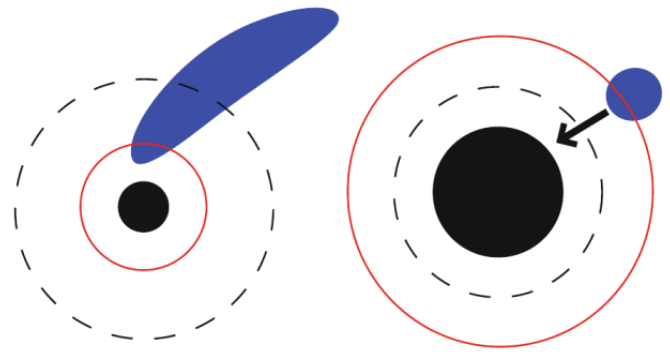
\includegraphics[scale=0.45]{nsbh}
                        \centering
                        \caption{Schematic pictures for the outcome of the merger process, depending on the relative position of $d_{tid}$ and $R_{ISCO}$. The solid filled circle denotes the BH, the distorted ellipsoid denotes the NS, the solid circle is the location of $R_{ISCO}$, and the dashed circle is the location of  $d_{tid}$. Left: the NS is tidally disrupted, and the spatial extent of the disrupted material is larger than or as large as that of the BH. Right: the NS is not tidally disrupted.}
                         \label{fig:nsbh}
                \end{figure}
        Tidal disruption occurs when the tidal force of the BH at the surface of the NS is stronger
        than the self-gravity of the NS. Assuming Newtonian gravity, this condition is approximately
                \begin{equation}
                        {{M_{NS}} \over {R_{NS}^2}} \sim {{3M_{BH}} \over {d_{tid}^3}}R_{NS}
                \end{equation}
        from which tidal disruption is simply $d_{tid} \sim (M_{BH}/M_{NS})^{1/3}R_{NS}$.
	Many factors influence the  tidal disruption of the NS: 
	it is more likely that the NS will be swallowed directly by a more massive BH, 
	since it exerts weaker tidal forces at the ISCO;
	a highly  spinning BH has the effect of reducing the ISCO radius,
	possibly beyond the NS Roche limit.
	Furthermore, the EOS of the NS can highly effect the conditions to power a SGRB:
	the softer the EOS, the larger the NS radius, the easier to power an EM counterpart,
	since the tidal force acting across the diameter of the star will be greater.

        A few tens of milliseconds after tidal disruption occurs the remnant consists of
        a remnant BH and tidal debris containing gravitationally bound and unbound matter.
        Some material gravitationally bound to the remnant swerves
        into an approximately axisymmetric disk around the BH, while some debris material,
        a large amount of neutron-rich material, is dynamically ejected and spread outwards at mildly relativistic speeds.
	 The accretion disk an spread to larger radii to conserve angular momentum in the rotational period $\sim 10 ms$,
        rather than being confined within the circularizing radius, resulting in a gradual mass infall into the BH over longer timescales, $\sim 0.1-1 s$.
        However, the mass accretion time scale is much longer than the rotational period, and hence, the disk remains quasi-stationary for $\gg 10 ms$.
        With the intention of obtaining accurate predictions for identifying and characterising NSBH mergers
        a model for the remnant mass outside the BH is needed.

        Since NSBH systems cover a high-dimensional and largely unconstrained parameter space,
        understanding whether or not these events can result in short GRBs emission requires to
        derive limits on the range of binary parameters leading to the disruption of a NS.
        Originally, Foucart proposed a model to calculate the amount of matter remaining
        outside the BH about $10ms$ after a BHNS merger, $M_{rem}$, based on comparison
        between $d_{tid}$ and $R_{ISCO}$:
                \begin{equation}
                \label{eq:mrem}
                        {{M_{rem}^{model}} \over {M^b_{NS}}} = \alpha(3q)^{1/3}(1 - 2C_{NS}) - \beta{{R_{ISCO}} \over {R_{NS}}}
                \end{equation}
        where $\alpha$ and $\beta$ are the free parameters of the model,
        and $M^b_{NS}$ is the baryon mass of the NS.
        Since applying the $d_{tid}$ derived from Newtonian gravity to compact object results in underestimating the $C_{NS}$,
        a more appropriate estimation of this quantity, in which compact objects are more strongly bound is
                \begin{equation}
                       \hat{d}_{tid} = d_{tid} (1 - 2C_{NS})
                \end{equation}
        This simple model applies to BH spins aligned with the orbital angular momentum and remnants below
        $\sim 20-25\%$ of the NS mass, leaving out unexplored regions of the parameter space,
        such as comparable masses and high spins.
        To better constraint $M_{rem}$, a new model was proposed by Foucart, Hinderer and Nissanke.
                \begin{equation}
                \label{eq:mremup}  
                        {{M_{rem}^{model}} \over {M^b_{NS}}} = \Bigg[ Max \Bigg( \alpha{{1 - 2C_{NS}} \over {\eta^{1/3}}} - \beta {{R_{ISCO}C_{NS}} \over{\eta M_{BH}}} + \gamma, 0 \Bigg)\Bigg]^{\delta}
                \end{equation}
        where $\alpha$, $\beta$, $\gamma$ and $\delta$ are the free parameter of the new model. \\
        Both models predict the $M_{rem}$ outside the BH after a NSBH merger,
        each result rely on tidal disruption dynamics considerations and
        is fitted to a set of numerical simulations,
        in order to assess their validity in the parameter space covered by the simulations.
        While model $\ref{eq:mrem}$ is tested against 26 numerical simulation covering mass ratios
        in the range $M_{BH}/M_{NS}=3-7$, $\chi_{BH}$ up to 0.9, and $R_{NS} \approx 11-16$km,
        model $\ref{eq:mremup}$ is fitted to 75 simulations covering the range $q = 1-7$ $\chi_{BH} =-0.5-0.97$,
        and $C_{NS} = 0.13-0.182$.
                \begin{figure}[H]
                        \noindent
                        \label{o3bankvso2bank}
                        \makebox[\textwidth]{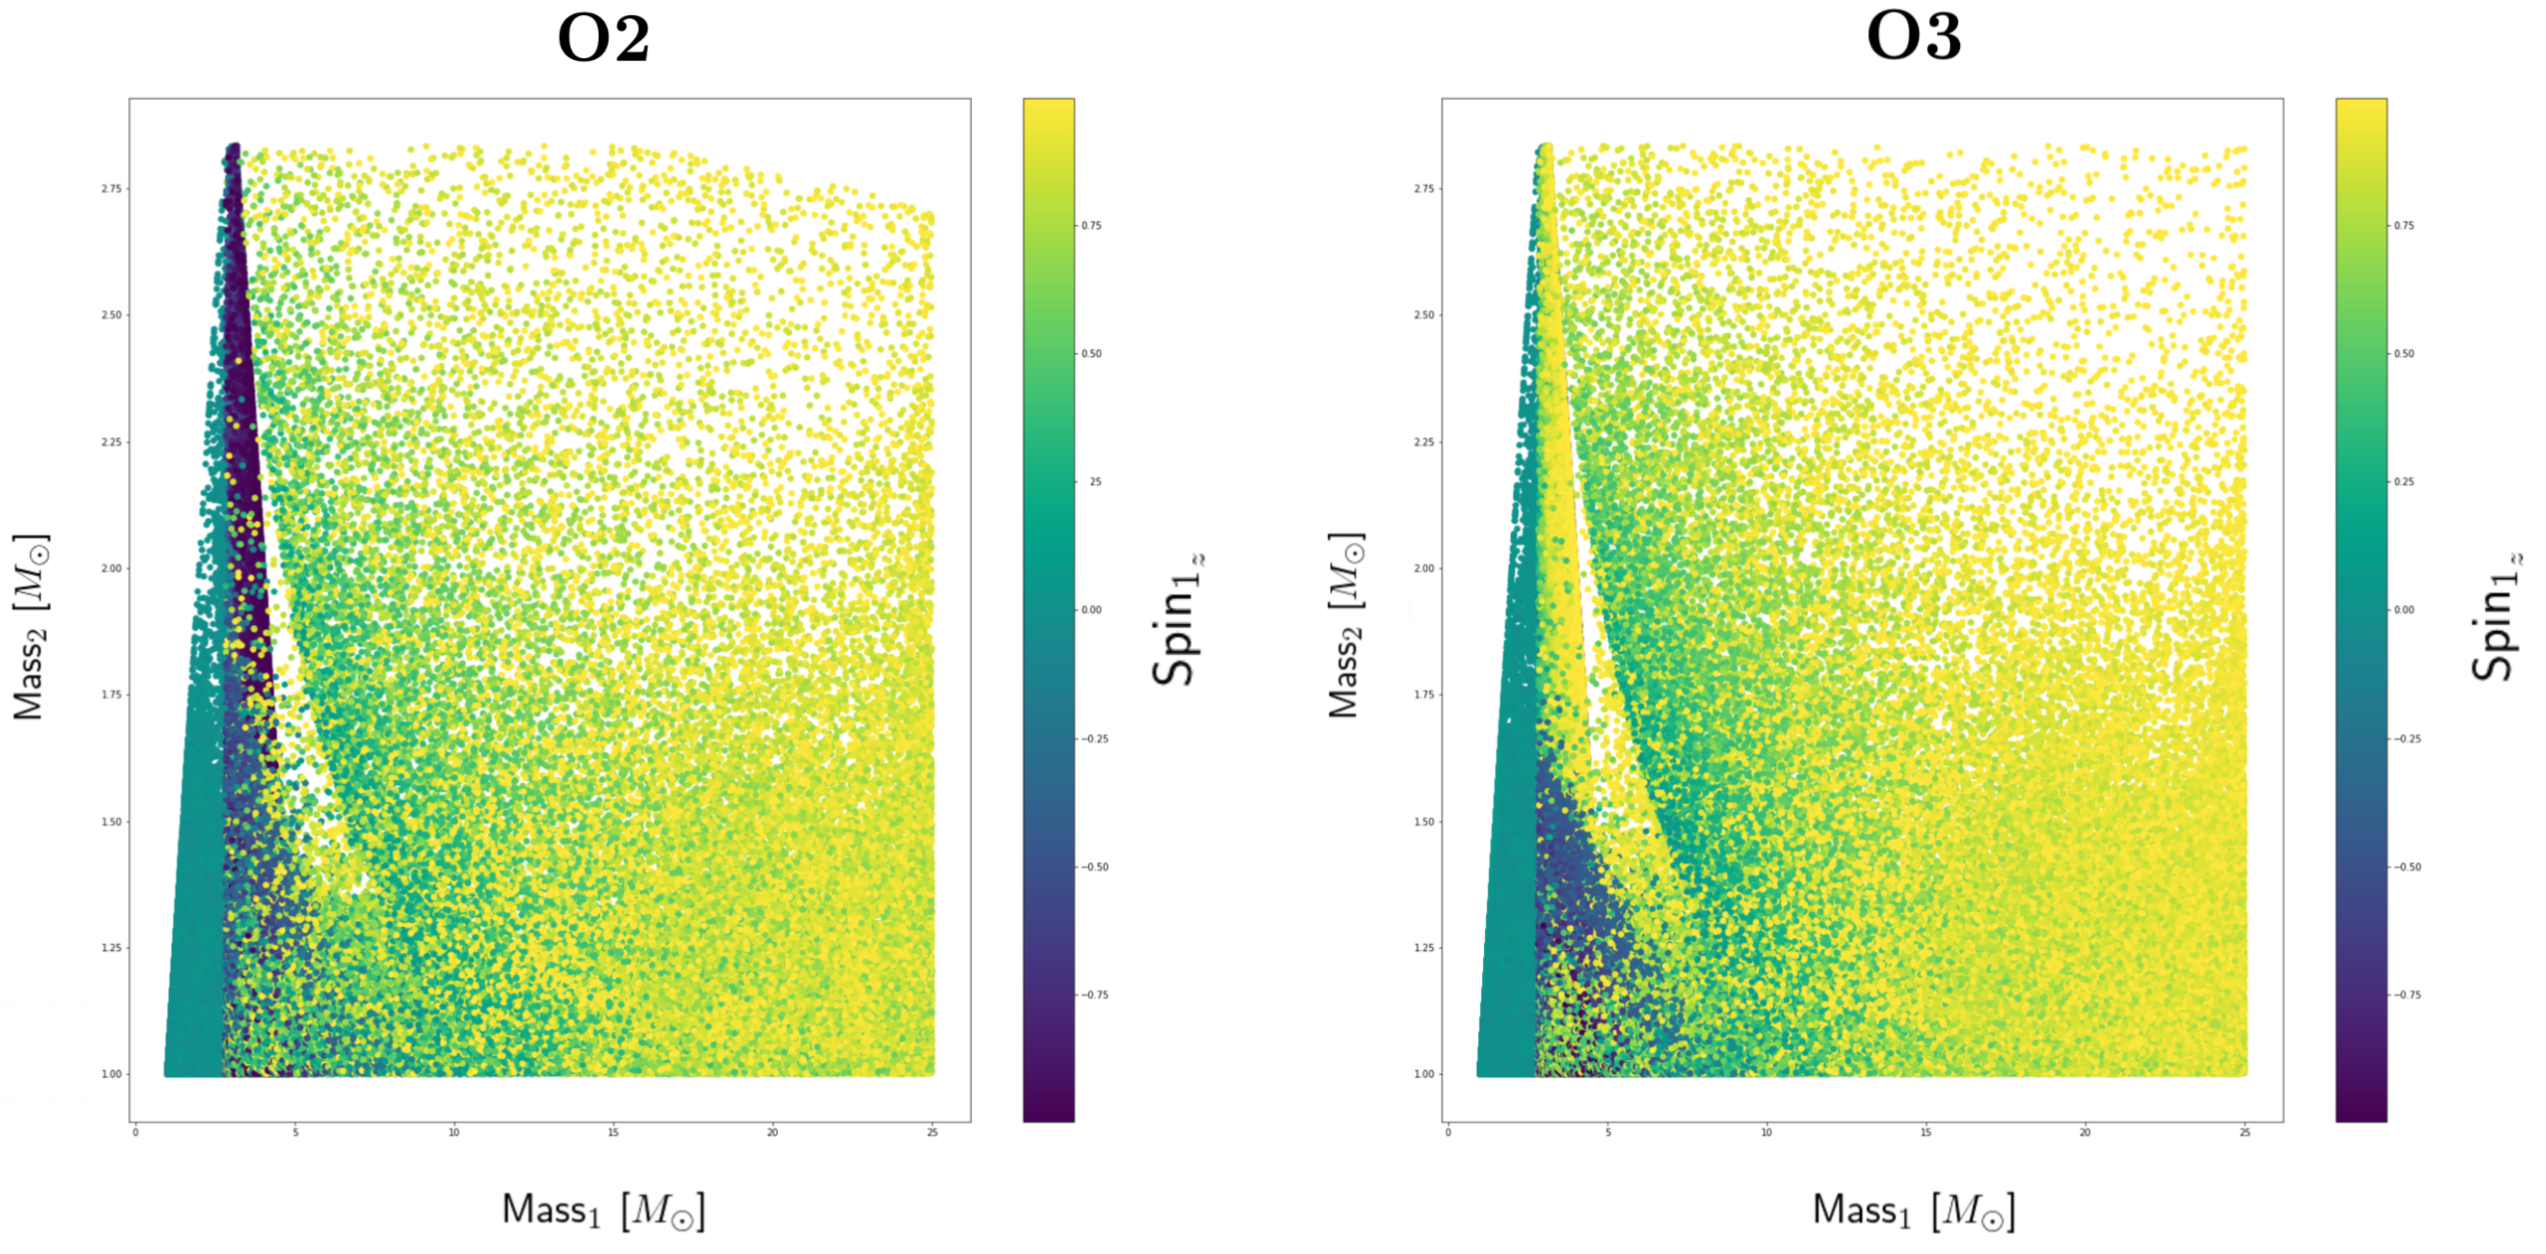
\includegraphics[scale=0.4]{o3bankvso2bank}}%
                        \centering
                        \caption{Comparison between the projection of the O2 and O3a search parameter space in the plane of the component masses, for the template bank generated with the old model $\ref{eq:mrem}$, and the updated one $\ref{eq:mremup}$, respectively.}
                        \label{fig:o3bankvso2bank}
                \end{figure}
        The new model covers previously unmodeled regions of the parameter space, comparable masses $q \sim 1$ and high spins,
        giving a more accurate  results.
	The benefits of updating the template bank with the new model, are shown in fig.$\ref{fig:o3bankvso2bank}$:
        the visible missing spot on the right high corner ($M_1 >  2.60 M_\odot$, $M_2 > 15 M_\odot $) of the O2 bank gets covered,
        which corresponds to high values of the component masses. 
	However, this particular region appears less dense than the rest of the mass parameter space, 
	because as the mass increases, the waveforms get shorter and start to overlap more with each other. \\
        An upgrade in the calculation for $q \sim 1$ binaries in order to distinguish BNS from low-mass NSBH,
        since a solar mass BH in a binary system with a NS companion could mimic the observable properties of a NSNS binary,
        is done by considering the two-body symmetry in vacuum gravity.
        When taking the limit $q \rightarrow \infty$ one loses the invariance under exchanging the bodies' labels,
        which can be restored by replacing $q^{-1}$ with $\eta$, as in Eq. $\ref{eq:mremup}$.
        This choice leads to a lager value for $R_{ISCO}$ when considering a binary with $q \sim 1$,
        which is physically expected because the accreting NS will begin its plunge at a $R_{ISCO}^{effective}$,
        causing the BH to grow, consequently the ISCO location for the remaining material outside will change,
        leading to a fractional change in the position of the ISCO for smaller $q$.
        This gives a more precise estimation for $M_{rem}$, which was previously overestimated for nearly equal-mass NSBH.

        This is clearly shown in the region $M_2 \leq 2.5$ of fig.$\ref{fig:o3bankvso2bank}$, where there is a slighty denser coverage.
        Furthermore, while Eq. $\ref{eq:mrem}$ did not consider nonlinear effects taking place after the coalescence of a NS
        with a rapidly spinning BH, leading to an underestimation of $M_{rem}$,
        the introduction of the new free parameters $\gamma$ and $\delta$ accurately predicts that in this scenario,
        the remnant mass has larger values than previously found and therefore it is more likely to have an EM counterpart.
\section{Bank Tests}
        The new template bank generates a large set of point within the mass and spin parameter space,
        with the desired minimum $M_{rem}$, then it checks if the systems produce an EM counterpart.
        This means they are required to produce a remnant mass disk:
        if they do EOS data are loaded and the minimum $\eta$ needed to generate a given $M_{rem}$,
        as a function of $M_{NS}$ and $\chi_{BH}$,  is computed;
        if this is not the case the binary is treated as point particle binaries.
        All system that produce the given $M_{rem}$ make the cut and are stored:
        as the EM cut can remove several randomly generated binaries,
        the numbers of accepted points needs to be tracked and stopped when they are enough.
        First all EM dark systems needs to be identified using the logical mask ‘\textbf{{\color{red}mask\_not\_bbh}},
        which track points that are not BBH: a point is kept if the secondary object is not a BH,
        then its masses and spins are stored.
        After this first cut only BNS and NSBH systems are left.
        To discriminate between these two classes, another requirement is that the secondary mass is a NS,
        so that ‘\textbf{{\color{green}mask\_bns}}’ identifies only BNS, while the systems that do not satisfy this conditions
        are identified by ‘\textbf{{\color{black}masknsbh}}’.
        All these point’s masses and spin are stored.
        As previously showed in Sec.$\ref{subsec:mrem}$, not all NSBH coalescence produce an EM counterpart,
        so the next step is to keep only those systems whose $M_{rem}$ is greater than the threshold mass to have a counterpart,
        identify these points with ‘\textbf{{\color{blue}mask\_nsbh\_bright}}’ and store their masses and spins.
\begin{table}[H]
\noindent
\begin{tabular}{|l|l|l|l|l|} \hline
\textbf{BNS}  & \textbf{NSBH}       & \textbf{NSBH}    & \textbf{BBH}     \\
EM-bright     & EM-bright  & EM-dim  & EM-dim  \\\hline
{\color{red}1}0{\color{green}1}  & {\color{red}1}1{\color{green}0}{\color{blue}1}  & {\color{red}1}1{\color{green}0}{\color{blue}0}  & {\color{red}0}  \\ \hline
\end{tabular}
\end{table}
		
	The O3a EM-bright template bank, viewed in the black hole mass-spin plane, is shown in Fig.$\ref{fig:banktest}$:
        a conspicuous section of the parameter space (lower-right) is empty of any templates,
        since greater BH masses and larger anti-aligned spins will not result in disruption of the NS before merger.\\ 
        The template bank is built with a hybrid geometric random method and uses templates generated with an aligned spin model,
        IMRPhenomD \cite{205}, a family of waveforms tuned for small mass ratios with aligned spins,                                                                                                        
        for non precessing point particle binaries.\\
	The template bank is designed to have an SNR loss of no more than 3\% due to discretisation, 
	which results in a bank of 288,177  templates. Filtering is performed from 27 Hz to 1000 Hz. 	
	Since the targeted search puts particular emphasis on the coalescence of  BNS and NSBH systems,
	it is important that the EM bright bank appropriately covers the region of the parameter space 
	that is expected to include the progenitors of short GRB and does not expand over this region,
	as this will increase the the computational cost of the analysis as well as the number of background triggers. \\ 
	It is also crucial to properly define the parameter space for the binary components based on astrophysical knowledge:
	combining the theoretical and experimental upper bound, the NS mass is restricted in the range $1M_\odot \leq M_{NS}  \leq 2.8M_\odot$,
	while the dimensionless spin magnitude to $\leq 0.05$, which is based on NS parameters from known Galactic BNS systems \cite{206},
       	In a similar fashion, the parameters range for the BH is chosen to be $1M_\odot \leq M_{BH}  \leq 25M_\odot$ and $0 \leq \chi_{BH} \leq 0.998$.
	Another restriction for the template bank to reduce background triggers and computation time, 
	is to consider only waveforms from binaries with orbital inclination angles of $\ang{0}$ or $\ang{180}$ \cite{46}. 
		\begin{figure}[H]
                        \noindent
                        \label{banktest}
                        \makebox[\textwidth]{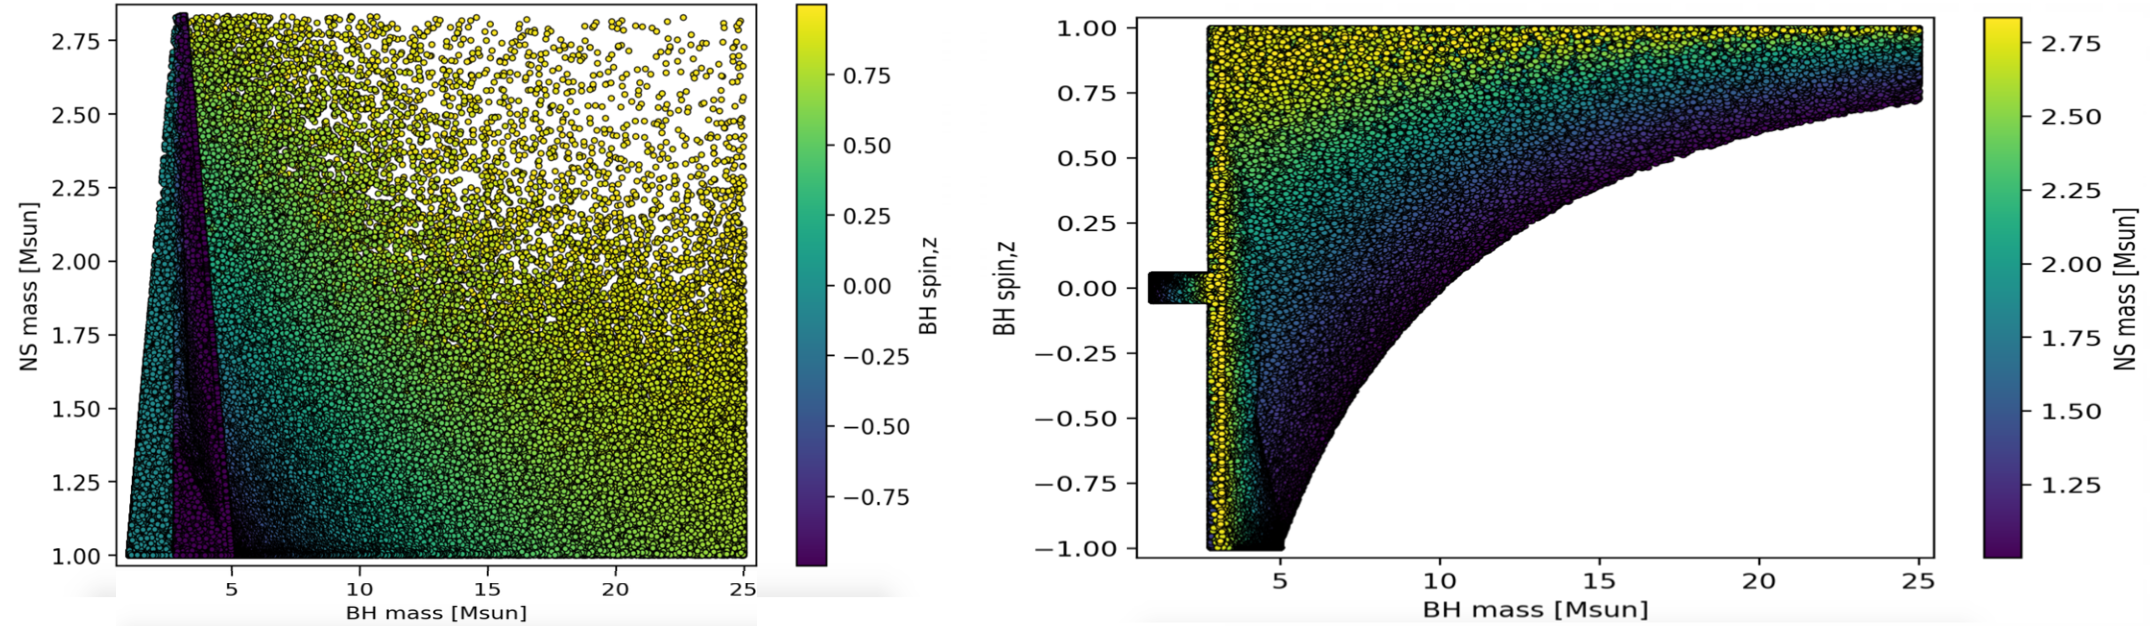
\includegraphics[scale=0.45]{banktest}}%
                        \centering
                        \caption{Parameter space boundaries for the O3a template bank illustrated through the BH spin vs BH mass.}
                        \label{fig:banktest}
                \end{figure}
	The effectiveness of the bank, in recovering the signal it searching for,
        can be assessed by calculating the fitting factor,
        already introduced in Sec.$\ref{subsec:fittingfactor}$.
        This is done by injecting two sets of known GW signals, broad and point injections,
        and determine how well the bank recovers them.
	The broad injections cover the entire BNS and NSBH parameter space and contains 10,000 injection signals each,
	approximated by the effective-one-body waveform model SEOBNRv4\_ROM, 
	which results to be faster during the bank simulation.\\
	The NSBH injection set is injected  through the same EM-bright condition so that
	only potentially EM-bright source waveforms are used to tune the pipeline and test its efficiency at making detections.
	The range of mass and spin parameters of the injected signals were chosen 
	to be the same as that of the bank and were drawn from a uniform distribution in this range. 
	The necessary requirements the bank must meet to be claimed effective are: 
	it needs to recover 99\% of injected signals is designed for with a fitting factor of 0.97 or better,
	no fitting factors with matches less than 0.95 should be present or 
	below 0.97 should not be clustered in a particular part of parameter space. 
	However, these conditions are not sufficient for the bank to  successfully recover all possible signals in the parameter region,
	since there may be different reasons why the template generation is not successful, such as different sensitivities in the two detectors, 	
	different waveform approximants, precession effects, tidal deformation, etc.\\
	The results are shown in Fig.$\ref{fig:fittingfactor}$: 
	the majority of fitting factors are above 0.97, 
	however, since the injection model is different from the one used to construct the template bank
	fitting factors down to 0.965 across the parameter space are present as expected.
	The first and fourth plot show that the bank performs well to match the injected signals 
	throughout the parameter space for NSBH and BNS systems, 
	except for those regions where both masses are high or for anti-aligned spins components.
	This could be explained as the placement method not performing properly in extreme regions of parameter space.
	From the missing clustering around points of either of the parameter spaces,
	the bank should not contain any systematic holes in its sensitivity.
		\begin{figure}[H]
                        \noindent
                        \label{fittingfactor}
                        \makebox[\textwidth]{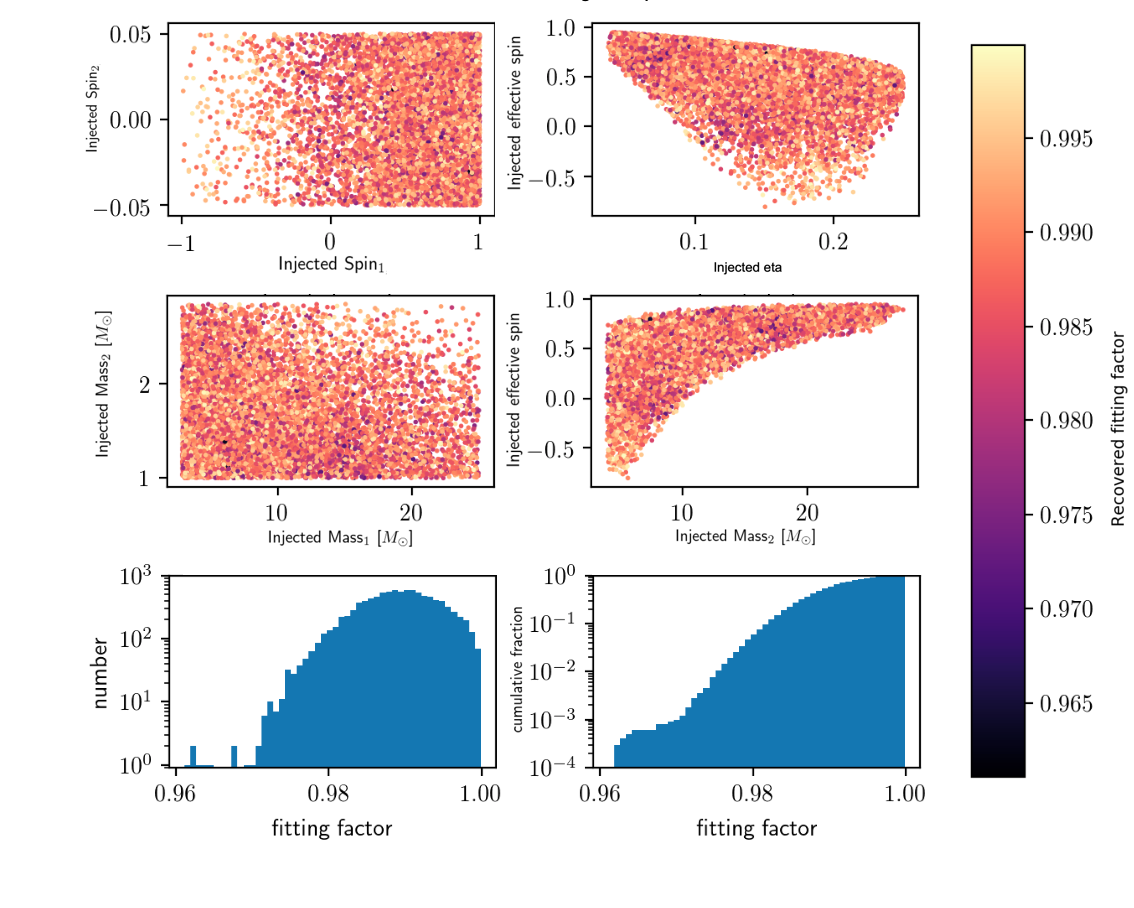
\includegraphics[scale=0.9]{fittingfactor}}%
                        \centering
                        \caption{Broad Injection set results. From top left to bottom right the plots are as follows: The first plot is of the fitting factors over the spin parameter space. The next plot is the fitting factors over the effective spin vs symmetric mass ratio $\eta$ parameter space. The third plot contains the the fitting factors over the mass parameter space. 
Plot four shows the fitting factor over the injected spin vs the secondary component mass. Plot five is a histogram of number of fitting factors per bin of fitting factors. The last plot has all the same data as the previous but is cumulative to determine percentages.}
                        \label{fig:fittingfactor}
                \end{figure}
	The average fitting factor for the entire bank is $\sim0.98$, that means a loss of detection rates of $\sim6\%$,
	because the detection rate  is proportional to the cube of the SNR, and SNR $\propto FF$.
	Since the analysis depends also on the extrinsic parameters such as sky-location and source distance,
	this is an ideal recovery rate.

	In Fig.$\ref{fig:pointinj}$, results from an additional check for the bank validity are shown: 
	this is done by using point injections, wherein 10,000 signals are injected at single points in the mass parameter space while varying the spins. 
	For this set, 43 points in the mass parameter space were chosen randomly. 
	It confirms that the bank works well, as the lowest fitting factor of these points is 0.9870, 
	which is consistent with the bank average from the broad injection set. 
                \begin{figure}[H]
                        \noindent
                        \label{pointinj}
                        \makebox[\textwidth]{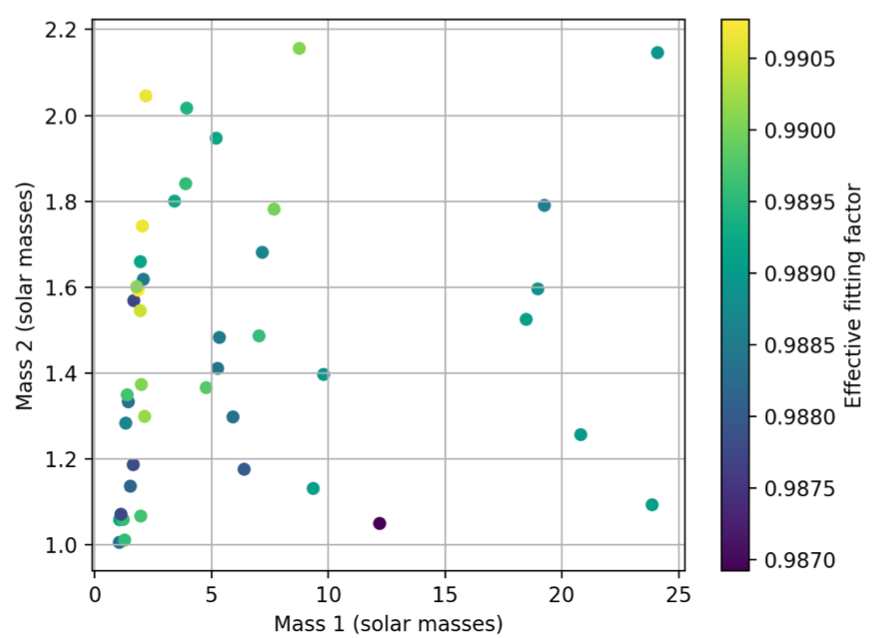
\includegraphics[scale=0.55]{pointinj}}%
                        \centering
                        \caption{The effective fitting factor is the signal-strength weighted average fitting factor. This is shown, as a function of masses, for the input injection sets. Injections are filtered so that only those passing the filter function used when creating the input files are considered. Usually this is used to restrict to only signals that are the parameter space used to create the template bank. Any point marked with a black cross contain no injections that pass the filter function.}
                        \label{fig:pointinj}
                \end{figure}

\section{O3 offline {\ttfamily PyGRB} analysis}
\label{sec:pygrb}
	The {\ttfamily PyGRB} pipeline performs a targeted search for CBC GW signals in LIGO and Virgo data associated with SGRBs seen by Swift and Fermi,
        using the known sky location of the SGRB and the relative GW detector sensitivities to analyses the data coherently, as described in $\ref{subsec:coherent}$.
        Even though this approach is more computationally expensive than a coincident search $\ref{subsec:coincident}$,
        it is more sensitive.
	The analysis is performed if at least two IFOs are active at the time the SGRB was observed, 
	and if the supplied data cover a sufficiently long period of time either side of the SGRB.
	The pipeline looks for a GW signal in a time window, “on-source”, that covers  5 s before to 1 s 
	after the Earth crossing time of the SGRB.
	However, in order to ensure that the detectors were operating stably at this time, 
	additional data is required to provide a good estimate of the detector sensitivity. 
	The first part of the analysis consists in matched-filtering the individual detector data;
	knowing sky location of the GRB and the fact that gravitational waves travel at the speed of light,
	data from each detector is then time-shifted so that there is a temporal coincidence between the GW and the GRB in each IFO.
	A list of triggers is assembled by keeping only times when the individual detector $\rho > 4$,
	and discarding any trigger that is not coincident in at least two detectors in the network. 
	Further trigger selection get accomplished after calculating the $\rho_{coinc}$, 
	and rejecting any trigger with $\rho_{coinc}<6$, and then repeating the same procedure for the $\rho_{coh}$.
	The last cut is done by computing the $\rho_{null}$ and keeping only the triggers that satisfy the following conditions:
		\begin{equation}
			\rho_{null} \leq 5.25 \hspace*{2cm} \text{and} \hspace*{2cm} \rho_{coh} \leq 20
		\end{equation}
		\begin{equation}
			\rho_{null} \leq {{\rho_{coh}-20}\over {5}} \hspace*{2cm} \text{and} \hspace*{2cm} rho_{coh} > 20
		\end{equation}
	This prevents losing possibile loud GW events, that have high $\rho_{null}$ and $\rho_{coh}$ values,
	because differences between the actual GW waveform and the template used for the matched filter, 
	as well as inaccuracies in timing and sky position, can all lead to some fraction of the energy of a GW contributing to the null SNR. 	
	From April 2019 to September 2019, the Advanced LIGO  and  Advanced  Virgo detectors undertook 
	the first part of the third observing run (O3a).
	PyGRB was used to search for GWs associated with short and ambiguous duration GRBs detected during O3a. 
	The GRBs analysed here were detected by Swift BAT or Fermi GBM.

\subsection{GRB190425089}
		\begin{figure}[H]
                        \noindent
                        \label{scienceseggrb1}
                        \makebox[\textwidth]{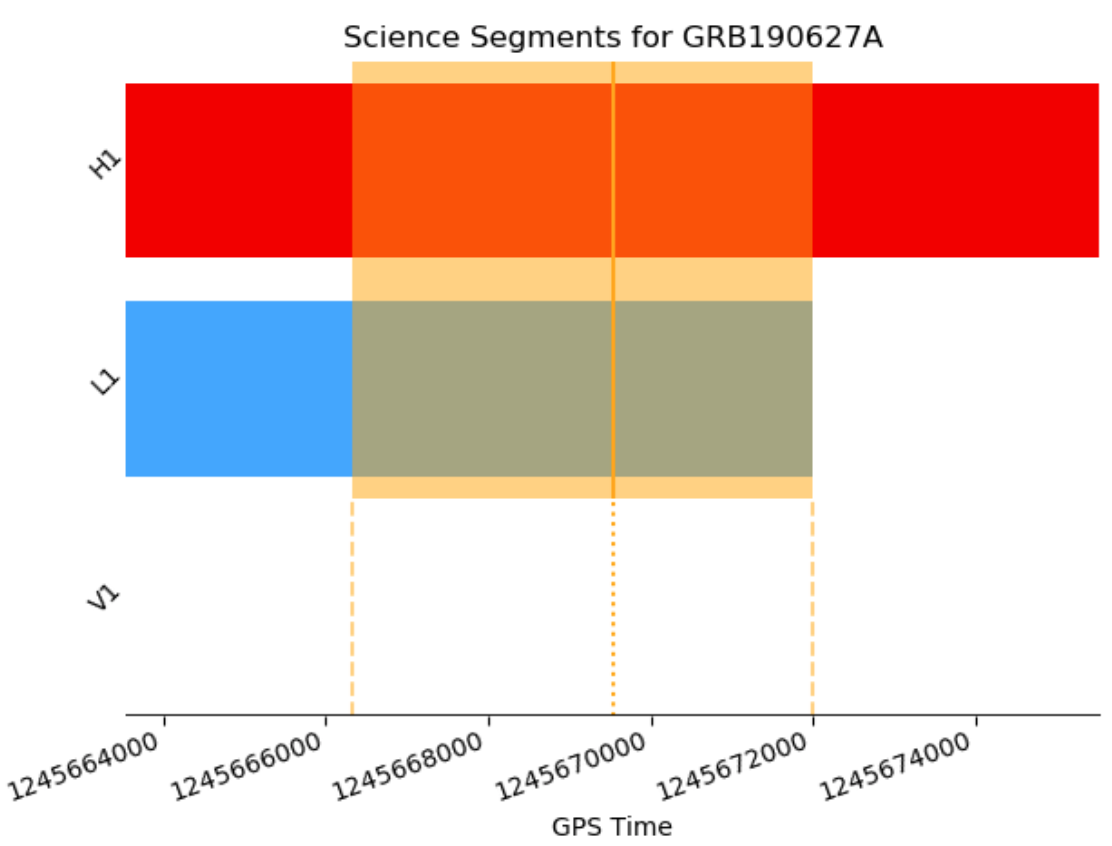
\includegraphics[scale=0.3]{scienceseggrb1}}%
                        \centering
	 		\caption{}
                        \label{fig:scienceseggrb1}
                \end{figure}





\subsection{GRB190627A}

\subsection{GRB190728271}

\section{{\ttfamily PyCBC} O3 HL C00 data preliminary runs}
\label{sec:pycbc00}
\subsection{Chunk 29}

%--------------------------------------------------------
\chapter*{Conclusions}
\addcontentsline{toc}{chapter}{Conclusions}
\markboth{Introduction}{Conclusions}

\fpg{Giri di correzione: 0.}%

\backmatter
\cleardoublepage

\phantomsection % Give this command only if hyperref is loaded \addcontentsline{toc}{chapter}{\bibname}

\begin{thebibliography}{500}

	\bibitem{1} Albert Einstein. On the General Theory of Relativity. Sitzungsber. Preuss. Akad. Wiss. Berlin (Math. Phys.), 1915:778–786, 1915. [Addendum: Sitzungsber. Preuss. Akad. Wiss. Berlin (Math. Phys.)1915,799(1915)]. 
	\bibitem{2} Albert Einstein. Naherungsweise integration der feldgleichungen der gravitation. Sitzungsberichte der Koniglich Preu{\ss}ischen Akademie der Wissenschaften (Berlin), 1:688–696, 1916. 
	\bibitem{3} M. Maggiore. Gravitational Waves: Volume 1: Theory and Experiments. Oxford University Press, 2008
	\bibitem{4} E. E. Flanagan and S.A .Hughes. The basics of gravitational wave theory. arXiv:gr-qc/0501041v3
	\bibitem{5} M. Blau, “Lecture Notes on General Relativity,” ICTP (2000). 
	\bibitem{6} Tjonnie G. F. Li. A. Extracting Physics from Gravitational Waves: Testing the Strong-field Dynamics of General Relativity and Inferring the Large-scale Structure of the Universe. Springer, 3 lug 2015	
	\bibitem{7} J. Weber. Detection and generation of gravitational waves. Phys. Rev., 117: 306–313, Jan 1960. doi:10.1103/PhysRev.117.306. 
	\bibitem{8} Gertsenshtein M.E.; Pustovoit V.I. On the detection of low frequency gravitational waves. Sov. J. Exp. Theor. Phys. 1962, 43, 605–607. 
	\bibitem{9} Yu, Haocun and others. Quantum correlations between the light and kilogram-mass mirrors of LIGO. [arXiv:2002.01519 [quant-ph]].
	\bibitem{10} Weinstein, A. Advanced LIGO optical configuration and prototyping effort. Class. Quantum Grav. 19, 1575–1584 (2002).
	\bibitem{11} D. G. Blair, E. J. Howell, L. Ju, C. Zhao. Advanced Gravitational Wave Detectors. Cambridge University Press, 16 feb 2012 
	\bibitem{12} Stephen Fairhurst. Triangulation of gravitational wave sources with a network of detectors. arXiv:0908.2356v2 [gr-qc]
	\bibitem{13} The LIGO Scientific Collaboration, the Virgo Collaboration. GWTC-1: A Gravitational-Wave Transient Catalog of Compact Binary Mergers Observed by LIGO and Virgo during the First and Second Observing Runs.arXiv:1811.12907v3 [astro-ph.HE]
	\bibitem{14} The LIGO Scientific Collaboration, the Virgo Collaboration. GW150914: First results from the search for binary black hole coalescence with Advanced LIGO. arXiv:1602.03839v3 [gr-qc]
        \bibitem{15} B.P. Abbott et al. (LIGO Scientific Collaboration and Virgo Collaboration). GW170817: Observation of Gravitational Waves from a Binary Neutron Star Inspiral. Phys. Rev. Lett. 119, 161101.	
	\bibitem{16} Charles W. Misner, Kip S. Thorne, and John Archibald Wheeler. Gravitation. W. H. Freeman, 1973
	\bibitem{17} Sean M. Carroll. Lecture Notes on General Relativity. arXiv:gr-qc/9712019v1
	\bibitem{18} B.S. Sathyaprakash, B.F. Schutz. Physics, Astrophysics and Cosmology with Gravitational Waves. arXiv:0903.0338v1 [gr-qc]
	\bibitem{19} Schutz, B. F. and Tinto, M. Antenna patterns of interferometric detectors of gravitational waves. I - Linearly polarized (ISSN 0035-8711), vol. 224, Jan. 1, 1987, p. 131-154.
	\bibitem{20} Francesco Zappa, Sebastiano Bernuzzi, Francesco Pannarale, Michela Mapelli, and Nicola Giacobbo. Black-Hole Remnants from Black-Hole–Neutron-Star Mergers. Phys. Rev. Lett. 123, 041102. 
	\bibitem{21} The LIGO Scientific Collaboration, the Virgo Collaboration. The basic physics of the binary black hole merger GW150914. arXiv:1608.01940v4 [gr-qc].
	\bibitem{22} C. J. Moore, R. H. Cole and C. P. L. Berry. Gravitational-wave sensitivity curves. Classical and Quantum Gravity, Volume 32, Number 1
	\bibitem{23} The LIGO Scientific Collaboration and the Virgo Collaboration. Tests of General Relativity with the Binary Black Hole Signals from the LIGO-Virgo Catalog GWTC-1. arXiv:1903.04467v3 [gr-qc].
	\bibitem{24} Bruce Allen. A chi-squared time–frequency discriminator for gravitational wave detection. Phys. Rev. D 71, 062001 (2005).
  	\bibitem{25} Collin Capano, Ian Harry, Stephen Privitera, and Alessandra Buonanno. Implementing a search for gravitational waves from non-precessing, spinning binary black holes. arXiv:1602.03509.
  	\bibitem{26} L. Wen et al 2008. Geometrical expression of the angular resolution of a network of gravitational-wave detectors and improved localization methods. J. Phys.: Conf. Ser. 122 012038.
	\bibitem{27} I. Harry, J. Calderon Bustillo, and A. Nitz, (2017). Searching for the full symphony of black hole binary mergers. arXiv:1709.09181 [gr-qc]. 
  	\bibitem{28} Samantha A. Usman et al. The PyCBC search for gravitational waves from compact binary coalescence.  Classical Quantum Gravity 33, 215004 (2016). 
  	\bibitem{29} Javier Roulet, Liang Dai, Tejaswi Venumadhav, Barak Zackay, and Matias Zaldarriaga. Template bank for compact binary coalescence searches in gravitational wave data: A general geometric placement algorithm. Phys. Rev. D 99, 123022. 
	\bibitem{30} S. Babak, R. Balasubramanian, D. Churches, T. Cokelaer, and B. S. Sathyaprakash. A template bank to search for gravitational waves from inspiralling compact binaries. I: Physical models. Class. Quant. Grav., 23:5477–5504, 2006. 
	\bibitem{31} Benjamin J. Owen, B. S. Sathyaprakash. Matched filtering of gravitational waves from inspiraling compact binaries: Computational cost and template placement. arXiv:gr-qc/9808076v1
	\bibitem{32} P. Ajith, N. Fotopoulos, S. Privitera, A. Neunzert, N. Mazumder, A. J. Weinstein. An effectual template bank for the detection of gravitational waves from inspiralling compact binaries with generic spins. arXiv:1210.6666v2.
	\bibitem{33} B. J. Owen. Search templates for gravitational waves from inspiraling binaries: Choice of template spacing. Phys. Rev. D 53, 6749 (1996). 
	\bibitem{34} I. W. Harry, B. Allen, and B. S. Sathyaprakash. A stochastic template placement algorithm for gravitational wave data analysis. Phys. Rev. D 80, 104014 (2009).  
	\bibitem{35} S. Roy, A. S. Sengupta, and N. Thakor. A hybrid geometric-random template placement algorithm for gravitational wave searches from compact binary coalescences. Phys. Rev. D 95, 104045 (2017). 
	\bibitem{36} N. Indik, K. Haris, T. Dal Canton, H. Fehrmann, B. Krishnan, A. Lundgren, A. B. Nielsen, and A. Pai. A stochastic template bank for gravitational wave searches for precessing neutron-star--black-hole coalescence events. Phys. Rev. D95, 064056 (2017), arXiv:1612.05173 [gr-qc].  
	\bibitem{37} Maccarone, T., and Knigge, C. Compact objects in globular clusters. Astron. Geophys. 48 5.12- 5.20 (2007)
	\bibitem{38} Harry I, Privitera S, Bohé A, Buonanno A (2016) Searching for gravitational waves from compact binaries with precessing spins. Phys Rev D 94:024012. https://doi.org/10.1103/PhysRevD.94.024012. arXiv:1603.02444
	\bibitem{39} Katerina Chatziioannou, Antoine Klein, Nicolás Yunes, and Neil Cornish. Constructing gravitational waves from generic spin-precessing compact binary inspirals. Phys. Rev. D 95, 104004
	\bibitem{40} L. K. Nuttall, T. J. Massinger, J. Areeda, J. Betzwieser, S. Dwyer, A. Effler, R. P. Fisher, P. Fritschel, J. S. Kissel, A. P. Lundgren, D. M. Macleod, D. Martynov, J. McIver, A. Mullavey, D. Sigg, J. R. Smith, G. Vajente, A. R. Williamson, C. C. Wipf. Improving the data quality of Advanced LIGO based on early engineering run results. arXiv:1508.07316v2 [gr-qc].
	\bibitem{41} Alexander H Nitz. Distinguishing short duration noise transients in LIGO data to improve the PyCBC search for gravitational waves from high mass binary black hole mergers. arXiv:1709.08974v2 [gr-qc].
	\bibitem{42} The LIGO Scientific Collaboration, the Virgo Collaboration. Effects of Data Quality Vetoes on a Search for Compact Binary Coalescences in Advanced LIGO's First Observing Run. arXiv:1710.02185v4 [gr-qc].
	\bibitem{43} Gareth S. Davies, Thomas Dent, Márton Tápai, Ian Harry, Connor McIsaac, Alexander H. Nitz. Extending the PyCBC search for gravitational waves from compact binary mergers to a global network. arXiv:2002.08291v2 [astro-ph.HE].
	\bibitem{44} LIGO Scientific, Virgo Collaboration, B. P. Abbott et al., A guide to LIGO-Virgo detector noise and extraction of transient gravitational-wave signals, Class. Quant. Grav. 37 (2020) 055002, [arXiv:1908.11170]. 
	\bibitem{45} Macleod D., Harry I. W. and Fairhurst S. A fully-coherent all-sky search for gravitational-waves from compact binary coalescences. 2016 Phys. Rev. D93 064004. 
	\bibitem{46} Williamson A., Biwer C., Fairhurst S. et al. Improved methods for detecting gravitational waves associated with short gamma-ray bursts. 2014 PhRvD 90 122004.
	\bibitem{47} S. Babak et al. Searching for gravitational waves from binary coalescence. Phys. Rev. D 87, 024033.
	\bibitem{48} Juan Calderón Bustillo, Francesco Salemi, Tito Dal Canton, and Karan P. Jani.Sensitivity of gravitational wave searches to the full signal of intermediate-mass black hole binaries during the first observing run of Advanced LIGO. Phys. Rev. D 97, 024016.
	\bibitem{49} Carl-Johan Haster, Zhilu Wang, Christopher P. L. Berry, Simon Stevenson, John Veitch, Ilya Mandel. Inference on gravitational waves from coalescences of stellar-mass compact objects and intermediate-mass black holes. https://doi.org/10.1093/mnras/stw233.
	\bibitem{50} C. Biwer et al. Validating gravitational-wave detections: The Advanced LIGO hardware injection system. Phys. Rev. D 95, 062002.
	\bibitem{51} Vassiliki Kalogera and Albert Lazzarini. LIGO and the opening of a unique observational window on the universe. PNAS March 21, 2017 114 (12) 3017-3025.
	\bibitem{52} Abbott, B. P. et al. (LIGO Scientific Collaboration, Virgo Collaboration). Observation of gravitational waves from a binary black hole merger. Phys. Rev. Lett. 116, 061102 (2016).
	\bibitem{53} KAGRA Collaboration, LIGO Scientific Collaboration, and Virgo Collaboration. Prospects for observing and localizing gravitational-wave transients with Advanced LIGO, Advanced Virgo and KAGRA (2019). Preprint at https://arxiv.org/abs/1304.0670. 
         \bibitem{54} Chen, H.-Y. et al. Distance measures in gravitational-wave astrophysics and cosmology (2017). arXiv:1709.08079.
	\bibitem{55} LIGO Scientific Collaboration and Virgo Collaboration et al. 2017b. Gravitational Waves and Gamma-rays from a Binary Neutron Star Merger: GW170817 and GRB 170817A.
	\bibitem{56} Abbott, B. P. et al. (LIGO Scientific Collaboration, Virgo Collaboration). Low-latency Gravitational-wave Alerts for Multimessenger Astronomy during the Second Advanced LIGO and Virgo Observing Run. ApJ 875, 161 (2019). 
	\bibitem{57} Abbott, B. P. et al. (LIGO Scientific Collaboration, Virgo Collaboration). GW150914: First Results from the Search for Binary Black Hole Coalescence with Advanced LIGO. Phys. Rev. D 93, 122003 (2016). 
	\bibitem{58} Abbott, B. P. et al. (LIGO Scientific Collaboration, Virgo Collaboration). GW151226: Observation of Gravitational Waves from a 22-Solar-Mass Binary Black Hole Coalescence. Phys. Rev. Lett. 116, 241103 (2016). 
	\bibitem{59} Abbott, B. P. et al. (LIGO Scientific Collaboration, Virgo Collaboration). Binary Black Hole Mergers in the First Advanced LIGO Observing Run. Phys. Rev. X 6, 041015 (2016).
	\bibitem{60} Abbott, B. P. et al. (LIGO Scientific Collaboration, Virgo Collaboration). GW170104: Observation of a 50-Solar-Mass Binary Black Hole Coalescence at Redshift 0.2. Phys. Rev. Lett. 118, 221101 (2017).
	\bibitem{61} Abbott, B. P. et al. (LIGO Scientific Collaboration, Virgo Collaboration). GW170814: A Three-Detector Observation of Gravitational Waves from a Binary Black Hole Coalescence. Phys. Rev. Lett. 119, 141101 (2017).
	\bibitem{62} Abbott, B. P. et al. (LIGO Scientific Collaboration, Virgo Collaboration). GW170817: Observation of Gravitational Waves from a Binary Neutron Star Inspiral. Phys. Rev. Lett. 119, 161101 (2017).         
	\bibitem{63} Abbott, B. P. et al. Multi-messenger observations of a binary neutron star merger. ApJ 848, L12 (2017).
	\bibitem{64} K. Belczynski, D. E. Holz, T. Bulik, and R. O’Shaugh- nessy, The First Gravitational-Wave Source from the Isolated Evolution of Two 40-100 Msun Stars, Nature (London) 534, 512 (2016)
	\bibitem{65} J. J. Eldridge and E. R. Stanway, BPASS Predictions for Binary Black-Hole Mergers, Mon. Not. R. Astron. Soc. 462, 3302 (2016).
	\bibitem{66} V. M. Lipunov, V. Kornilov, E. Gorbovskoy, N. Tiurina, P. Balanutsa, and A. Kuznetsov, The First Gravitational- Wave Burst GW150914. Part I. Scenario Machine Prediction, New Astron. 51, 122 (2016).
	\bibitem{67} S.E. de Mink and I. Mandel, The Chemically Homogeneous Evolutionary Channel for Binary Black Hole Mergers: Rates and Properties of Gravitational-Wave Events Detectable by Advanced LIGO, Mon. Not. R. Astron. Soc. 460, 3545 (2016).
 	\bibitem{68} K. Inayoshi, K. Kashiyama, E. Visbal, and Z. Haiman, Strong Gravitational Wave Background from Population III Binary Black Holes Consistent with Cosmic Reionization, Mon. Not. R. Astron. Soc. 461, 2722 (2016).
 	\bibitem{69} C. L. Rodriguez, C. J. Haster, S. Chatterjee, V. Kalogera, and F. A. Rasio, Dynamical Formation of the GW150914 Binary Black Hole, Astrophys. J. Lett. 824, L8 (2016). M. Mapelli, Massive Black Hole Binaries from Runaway Collisions: The Impact of Metallicity, Mon. Not. R. Astron. Soc. 459, 3432 (2016).
        \bibitem{70} I. Bartos, B. Kocsis, Z. Haiman, and S. Márka, Rapid and Bright Stellar-Mass Binary Black Hole Mergers in Active Galactic Nuclei, arXiv:1602.03831.
 	\bibitem{71} N. C. Stone, B. D. Metzger, and Z. Haiman, Assisted Inspirals of Stellar Mass Black Holes Embedded in AGN Disks, Mon. Not. R. Astron. Soc., doi: 10.1093/ mnras/stw2260 (2015).
       \bibitem{72} I. Mandel and S. E. de Mink, Merging Binary Black Holes Formed through Chemically Homogeneous Evolution in Short-Period Stellar Binaries, Mon. Not. R. Astron. Soc. 458, 2634 (2016).
         \bibitem{73} P. Marchant, N. Langer, P. Podsiadlowski, T. M. Tauris, and T. J. Moriya, A New Route Towards Merging Massive Black Holes, Astron. Astrophys. 588, A50 (2016).
     \bibitem{74}K. Belczynski, T. Bulik, and B. Rudak, The First Stellar Binary Black Holes: The Strongest Gravitational Wave Burst Sources, Astrophys. J. Lett. 608, L45 (2004).
       \bibitem{75} T. Kinugawa, K. Inayoshi, K. Hotokezaka, D. Nakauchi, and T. Nakamura, Possible Indirect Confirmation of the Existence of Pop III Massive Stars by Gravitational Wave, Mon. Not. R. Astron. Soc. 442, 2963 (2014).
         \bibitem{76} A. Tutukov and L. Yungelson, Evolution of Massive Close Binaries, Nauchnye Informatsii 27, 70 (1973).
         \bibitem{77} A. V. Tutukov and L. R. Yungelson, The Merger Rate of Neutron Star and Black Hole Binaries, Mon. Not. R. Astron. Soc. 260, 675 (1993).
        \bibitem{78} V. M. Lipunov, K. A. Postnov, and M. E. Prokhorov, Formation and Coalescence of Relativistic Binary Stars: The Effect of Kick Velocity, Mon. Not. R. Astron. Soc. 288, 245 (1997).
        \bibitem{79} R. Voss and T. M. Tauris, Galactic Distribution of Merging Neutron Stars and Black Holes—Prospects for Short Gamma-Ray Burst Progenitors and LIGO/Virgo, Mon. Not. R. Astron. Soc. 342, 1169 (2003).
        \bibitem{80} G. Nelemans, Galactic Binaries as Sources of Gravitational Waves, in Astrophysics of Gravitational Wave Sources, American Institute of Physics Conference Series, edited by J.M. Centrella (AIP, Melville, NY, 2003), Vol. 686, pp. 263–272.
         \bibitem{81} K. Belczynski, M. Dominik, T. Bulik, R. O’Shaughnessy, C. Fryer, and D. E. Holz, The Effect of Metallicity on the Detection Prospects for Gravitational Waves, Astrophys. J. Lett. 715, L138 (2010).
         \bibitem{82} B. McKernan, K. E. S. Ford, W. Lyra, and H. B. Perets, Intermediate Mass Black Holes in AGN DiscsI. Production and Growth, Mon. Not. R. Astron. Soc. 425, 460 (2012).
         \bibitem{83} J.M. Bellovary, M.-M. Mac Low, B. McKernan, and K. E. S. Ford, Migration Traps in Disks around Super- massive Black Holes, Astrophys. J. Lett. 819, L17 (2016).
         \bibitem{84} S. Sigurdsson and L. Hernquist, Primordial Black Holes in Globular Clusters, Nature (London) 364, 423 (1993).
        \bibitem{85} S. F. Portegies Zwart and S. L. W. McMillan, Black Hole Mergers in the Universe, Astrophys. J. 528, L17 (2000).
        \bibitem{86} M. C. Miller and V. M. Lauburg, Mergers of Stellar-Mass Black Holes in Nuclear Star Clusters, Astrophys. J. 692, 917 (2009).
        \bibitem{87} B. M. Ziosi, M. Mapelli, M. Branchesi, and G. Tormen, Dynamics of Stellar Black Holes in Young Star Clusters with Different Metallicities II. Black Hole-Black Hole Binaries, Mon. Not. R. Astron. Soc. 441, 3703 (2014).
         \bibitem{88} C.L. Rodriguez, M. Morscher, B. Pattabiraman, S. Chatterjee, C.-J. Haster, and F.A. Rasio, Binary Black Hole Mergers from Globular Clusters: Implications for Advanced LIGO, Phys. Rev. Lett. 115, 051101 (2015).
         \bibitem{89} C. P. L. Berry et al., Parameter Estimation for Binary Neutron-Star Coalescences with Realistic Noise During the Advanced LIGO Era, Astrophys. J. 804, 114 (2015).
 	\bibitem{90} S. Fairhurst, Source Localization with an Advanced Gravitational Wave Detector Network, Classical Quantum Gravity 28, 105021 (2011).
         \bibitem{91} L. P. Singer and L. R. Price, Rapid Bayesian Position Reconstruction for Gravitational-Wave Transients, Phys. Rev. D 93, 024013 (2016).
   	\bibitem{92} I. W. Harry,  S. Fairhurst, A targeted coherent search for gravitational waves from compact binary coalescences. 10.1103/PhysRevD.83.084002. 
    	\bibitem{93} B. P. Abbott, R. Abbott, T. D. Abbott et al. (LIGO Scientific Collaboration and Virgo Collaboration), Properties of the Binary Black Hole Merger GW150914, Phys. Rev. Lett. 116, 241102 (2016).
 	\bibitem{94} S. Vitale, R. Lynch, J. Veitch, V. Raymond, and R. Sturani, Measuring the Spin of Black Holes in Binary Systems Using Gravitational Waves, Phys. Rev. Lett. 112, 251101 (2014). 
 	\bibitem{95} M. V. van der Sluys, C. Roever, A. Stroeer, N. Christensen, V. Kalogera, R. Meyer, and A. Vecchio, Gravitational- Wave Astronomy with Inspiral Signals of Spinning Compact-Object Binaries,        Astrophys. J. 688, L61 (2008).
         \bibitem{96}S. Nissanke, D. E. Holz, S. A. Hughes, N. Dalal, and J. L. Sievers, Exploring Short Gamma-Ray Bursts as Gravitational-Wave Standard Sirens, Astrophys. J. 725, 496 (2010).
         \bibitem{97} B. Farr et al., Parameter Estimation on Gravitational Waves from Neutron-Star Binaries with Spinning Components, Astrophys. J. 825, 116 (2015).
    	\bibitem{98} C. Cutler and E. Flanagan, Gravitational Waves from Merging Compact Binaries: How Accurately Can One Extract the Binary’s Parameters from the Inspiral Waveform?, Phys. Rev. D 49, 2658 (1994) 
   	\bibitem{99} J. A. Gonzalez, U. Sperhake, B. Brügmann, M. Hannam, and S. Husa, Total Recoil: The Maximum Kick from Nonspinning Black-Hole Binary Inspiral, Phys. Rev. Lett. 98, 091101 (2007).
        \bibitem{100} E. Berti, V. Cardoso, J.A. Gonzalez, U. Sperhake, M. Hannam, S. Husa, and B. Brügmann, Inspiral, Merger and Ringdown of Unequal Mass Black Hole Binaries: A Multipolar Analysis, Phys. Rev. D 76, 064034 (2007).
         \bibitem{101} J. G. Baker, W. D. Boggs, J. Centrella, B. J. Kelly, S. T. McWilliams, and J.R. van Meter, Mergers of Non- spinning Black-Hole Binaries: Gravitational Radiation Characteristics, Phys. Rev. D 78, 044046 (2008). 
        \bibitem{102} C. Reisswig, S. Husa, L. Rezzolla, E.N. Dorband, D. Pollney, and J. Seiler, Gravitational-Wave Detectability of Equal-Mass Black-Hole Binaries with Aligned Spins, Phys. Rev. D 80, 124026 (2009). 
    	\bibitem{103} A. Taracchini, A. Buonanno, Y. Pan, T. Hinderer, M. Boyle et al., Effective-One-Body Model for Black-Hole Binaries with Generic Mass Ratios and Spins, Phys. Rev. D 89, 061502 (2014).
         \bibitem{104} M. Pürrer, Frequency Domain Reduced Order Model of Aligned-Spin Effective-One-Body Waveforms with Generic Mass-Ratios and Spins, Phys. Rev. D 93, 064041 (2016). 
        \bibitem{105} S. Husa, S. Khan, M. Hannam, M. Pürrer, F. Ohme, X. J. Forteza, and A. Bohé, Frequency-Domain Gravitational Waves from Nonprecessing Black-Hole Binaries. I. New Numerical Waveforms and Anatomy of the Signal, Phys. Rev. D 93, 044006 (2016).
         \bibitem{106}  S. Khan, S. Husa, M. Hannam, F. Ohme, M. Prrer, X. J. Forteza, and A. Boh, Frequency-Domain Gravitational Waves from Non-precessing Black-Hole Binaries. II. A Phenomenological Model for the Advanced Detector Era, Phys. Rev. D 93, 044007 (2016).
         \bibitem{107} M. Hannam, P. Schmidt, A. Bohé, L. Haegel, S. Husa, F. Ohme, G. Pratten, and M. Pürrer, Simple Model of Complete Precessing Black-Hole-Binary Gravitational Waveforms, Phys. Rev. Lett. 113, 151101 (2014).
         \bibitem{108} B. P. Abbott, R. Abbott, T. D. Abbott et al. (LIGO Scientific Collaboration and Virgo Collaboration), GW150914: The Advanced LIGO Detectors in the Era of First Discoveries, Phys. Rev. Lett. 116, 131103 (2016).
         \bibitem{109} T. Dal Canton et al., Implementing a Search for Aligned- Spin Neutron Star-Black Hole Systems with Advanced Ground Based Gravitational Wave Detectors, Phys. Rev. D 90, 082004 (2014).
 	\bibitem{110} S. A. Usman et al., An Improved Pipeline to Search for Gravitational Waves from Compact Binary Coalescence, arXiv:1508.02357.
        \bibitem{111} A. H. Nitz, I. W. Harry, J. L. Willis, C. M. Biwer, D. A. Brown, L. P. Pekowsky, T. Dal Canton, A. R. Williamson, T. Dent, C. D. Capano et al., PyCBC Software, https:// github.com/ligo!cbc/pycbc.
        \bibitem{112} K. Cannon, R. Cariou, A. Chapman, M. Crispin-Ortuzar, N. Fotopoulos et al., Toward Early-Warning Detection of Gravitational Waves from Compact Binary Coalescence, Astrophys. J. 748, 136 (2012).
 	\bibitem{113} S. Privitera, S. R. P. Mohapatra, P. Ajith, K. Cannon, N. Fotopoulos, M.A. Frei, C. Hanna, A.J. Weinstein, and J. T. Whelan, Improving the Sensitivity of a Search for Coalescing Binary Black Holes with Nonprecessing Spins in Gravitational Wave Data, Phys. Rev. D 89, 024003 (2014).
         \bibitem{114} C. Messick, K. Blackburn, P. Brady, P. Brockill, K. Cannon, S. Caudill, S. J. Chamberlin, J. D. E. Creighton, R. Everett, C. Hanna et al., Analysis Framework for the Prompt Discovery of Compact Binary Mergers in Gravi- tational-wave Data, arXiv:1604.04324
         \bibitem{115} A. Effler, R. M. S. Schofield, V. V. Frolov, G. Gonzalez, K. Kawabe, J. R. Smith, J. Birch, and R. McCarthy, Envi- ronmental Influences on the LIGO Gravitational Wave Detectors During the 6th Science Run, Classical Quantum Gravity 32, 035017 (2015). 
        \bibitem{116} B.P. Abbott et al. (LIGO Scientific Collaboration and Virgo Collaboration), Effects of Data Quality Vetoes on a Search for Compact Binary Coalescences in Ad- vanced LIGO’s First Observing Run 
        \bibitem{117} L. A. Wainstein and V. D. Zubakov, Extraction of Signals from Noise (Prentice-Hall, Englewood Cliffs, NJ, 1962). 
         \bibitem{118} K. S. Thorne, Gravitational Radiation, in Three Hundred Years of Gravitation, edited by S. W. Hawking and W. Israel (Cambridge University Press, Cambridge, England, 1987), Chap. 9, pp. 330–458. 
        \bibitem{119} B. S. Sathyaprakash and S. V. Dhurandhar, Choice of Filters for the Detection of Gravitational Waves from Coalescing Binaries, Phys. Rev. D 44, 3819 (1991). 
 	\bibitem{120} C. Cutler et al., The Last Three Minutes: Issues in Gravitational Wave Measurements of Coalescing Compact Binaries, Phys. Rev. Lett. 70, 2984 (1993).
 	\bibitem{121} C. E. Rhoades, Jr. and R. Ruffini, Maximum Mass of a Neutron Star, Phys. Rev. Lett. 32, 324 (1974). 
	\bibitem{122} V. Kalogera and G. Baym, The Maximum Mass of a Neutron Star, Astrophys. J. 470, L61 (1996). 
	\bibitem{123} F. Ozel, D. Psaltis, R. Narayan, and J. E. McClintock, The Black Hole Mass Distribution in the Galaxy, Astrophys. J. 725, 1918 (2010). 
	\bibitem{124} W. M. Farr, N. Sravan, A. Cantrell, L. Kreidberg, C. D. Bailyn, I. Mandel, and V. Kalogera, The Mass Distribution of Stellar-Mass Black Holes, Astrophys. J. 741, 103 (2011). 
	\bibitem{125} L. Kreidberg, C. D. Bailyn, W. M. Farr, and V. Kalogera, Mass Measurements of Black Holes in X-Ray Transients: Is There a Mass Gap?, Astrophys. J. 757, 36 (2012). 
	\bibitem{126} L. Blanchet, T. Damour, B. R. Iyer, C. M. Will, and A. G. Wiseman, Phys. Rev. Lett. 74, 3515 (1995).
	\bibitem{127} C. Cutler and E. E. Flanagan, Phys. Rev. D 49, 2658 (1994). 
	\bibitem{128} F. Ohme, A.B. Nielsen, D. Keppel, and A. Lundgren, Statistical and Systematic Errors for Gravitational-Wave Inspiral Signals: A Principal Component Analysis, Phys. Rev. D 88, 042002 (2013). 
	\bibitem{129} J. Antoniadis, P. C. C. Freire, N. Wex, T. M. Tauris, R. S. Lynch et al., A Massive Pulsar in a Compact Relativistic Binary, Science 340, 1233232 (2013). 
	\bibitem{130} K. Belczynski, A. Buonanno, M. Cantiello, C. L. Fryer, D. E. Holz, I. Mandel, M. C. Miller, and M. Walczak, The Formation and Gravitational-Wave Detection of Massive Stellar Black-Hole Binaries, Astrophys. J. 789, 120 (2014). 
	\bibitem{131} We quote the matched-filter SNR as computed by the PyCBC search using the updated calibration; the GstLAL values agree within 2\%. 
	\bibitem{132} C. E. Rhoades, Jr. and R. Ruffini, Maximum Mass of a Neutron Star, Phys. Rev. Lett. 32, 324 (1974).
        \bibitem{132} The LIGO Scientific Collaboration, the Virgo Collaboration. GW190412: Observation of a Binary-Black-Hole Coalescence with Asymmetric Masses. arXiv:2004.08342.
	\bibitem{134} B. P. Abbott et al. (LIGO Scientific Collaboration, Virgo Collaboration), Astrophysical Implications of the Binary Black-Hole Merger GW150914. Astrophys. J. Lett. 818, L22 (2016), arXiv:1602.03846 [astro-ph.HE]. 
	\bibitem{135} J. S. Vink, New Astron. Rev. 52, 419 (2008).
	\bibitem{136} B. P. Abbott et al. (LIGO Scientific Collaboration, Virgo Collaboration), Phys. Rev. X 6, 041015 (2016), arXiv:1606.04856 [gr-qc]. 
	\bibitem{137} B. P. Abbott et al. (LIGO Scientific Collaboration, Virgo Collaboration), Astrophys. J. Lett. 833, L1 (2016), arXiv:1602.03842 [astro-ph.HE]. 
	\bibitem{138} Cannon et al. 2015; Messick et al. 2017; Adams et al. 2016; Nitz et al. GW170608: Observation of a 19 Solar-mass Binary Black Hole Coalescence (2017b).
	\bibitem{139} Racine 2008; Ajith et al. 2011.
	\bibitem{140} Abbott et al. 2016e.
	\bibitem{141} Lattimer and Prakash 2016.
	\bibitem{142} Spera et al. 2015.
	\bibitem{143} K. Cannon et al., Astrophys. J. 748, 136 (2012).
	\bibitem{144} C. Messick et al., Phys. Rev. D 95, 042001 (2017).
	\bibitem{145} A. H. Nitz et al., PYCBC Software (GitHub, 2017) [https:// github.com/ligo-cbc/pycbc].
	\bibitem{146} A. H. Nitz, T. Dent, T. Dal Canton, S. Fairhurst, and D. A. Brown, arXiv:1705.01513.
	\bibitem{147} A. H. Nitz, arXiv:1709.08974.
	\bibitem{148} S. A. Usman et al., Classical Quantum Gravity 33, 215004 (2016).
	\bibitem{149} T. Dal Canton et al., Phys. Rev. D 90, 082004 (2014). 
	\bibitem{150} B. Allen, W. G. Anderson, P. R. Brady, D. A. Brown, and J. D. E. Creighton, Phys. Rev. D 85, 122006 (2012).
	\bibitem{151} S. Klimenko et al., Phys. Rev. D 93, 042004 (2016).
	\bibitem{152} J. Veitch et al., Phys. Rev. D 91, 042003 (2015).
	\bibitem{153} Meszaros, P. and Rees, M. J. Relativistic fireballs and their impact on external matter - Models for cosmological gamma-ray bursts. Astrophysical Journal, Part 1 (ISSN 0004-637X), vol. 405, no. 1, p. 278-284. 
	\bibitem{154} L. Blanchet, Living Rev. Relativity 17, 2 (2014).
	\bibitem{155} A. Buonanno and T. Damour, Phys. Rev. D 59, 084006 (1999).
	\bibitem{156} A. Buonanno and T. Damour, Phys. Rev. D 62, 064015 (2000).
	\bibitem{157} T. Damour, P. Jaranowski, and G. Schaefer, Phys. Rev. D 78, 024009 (2008).
	\bibitem{158} T. Damour and A. Nagar, Phys. Rev. D 79, 081503 (2009).
	\bibitem{159} A. Taracchini, A. Buonanno, Y. Pan, T. Hinderer, M. Boyle et al., Phys. Rev. D 89, 061502 (2014).
	\bibitem{160} M. Pürrer, Phys. Rev. D 93, 064041 (2016).
	\bibitem{161} S. Husa, S. Khan, M. Hannam, M. Pürrer, F. Ohme, X. J. Forteza, and A. Bohé, Phys. Rev. D 93, 044006 (2016). 
	\bibitem{162} Metzger, M et al. Spectral constraints on the redshift of the optical counterpart to the gamma-ray burst. 1997, Nature, 387, 878.
	\bibitem{163} M. Hannam, P. Schmidt, A. Bohé, L. Haegel, S. Husa, F. Ohme, G. Pratten, and M. Pürrer, Phys. Rev. Lett. 113, 151101 (2014).
	\bibitem{164} R. Smith, S.E. Field, K. Blackburn, C.-J. Haster, M. Pürrer, V. Raymond, and P. Schmidt, Phys. Rev. D 94, 044031 (2016).
	\bibitem{165} M. M. Kasliwal and S. Nissanke, Astrophys. J. 789, L5 (2014). 
	\bibitem{166} L. P. Singer, L. R. Price, B. Farr, A. L. Urban, C. Pankow et al., Astrophys. J. 795, 105 (2014). 
	\bibitem{167} C. P. L. Berry et al., Astrophys. J. 804, 114 (2015). 
	\bibitem{168} S. Fairhurst, New J. Phys. 11, 123006 (2009); 13, 069602 (E) (2011). 
 	\bibitem{169} S. Fairhurst, Classical Quantum Gravity 28, 105021 (2011). 
 	\bibitem{170} P. Ajith and S. Bose, Phys. Rev. D 79, 084032 (2009). 
 	\bibitem{171} D. M. Eardley, D. L. Lee, A. P. Lightman, R. V. Wagoner, and C. M. Will, Phys. Rev. Lett. 30, 884 (1973). 
 	\bibitem{172} D. M. Eardley, D. L. Lee, and A. P. Lightman, Phys. Rev. D 
 	\bibitem{173} J. M. Weisberg, D. J. Nice, and J. H. Taylor, Astrophys. J. 722, 1030 (2010).
 	\bibitem{174} P. C. C. Freire, N. Wex, G. Esposito-Farese, J. P. W. Verbiest, M. Bailes, B. A. Jacoby, M. Kramer, I. H. Stairs, J. Antoniadis, and G. H. Janssen, Mon. Not. R. Astron. Soc. 423, 3328 (2012).
 	\bibitem{175} I. H. Stairs, Living Rev. Relativity 6, 5 (2003).
 	\bibitem{176} N. Wex, arXiv:1402.5594.
	\bibitem{177} K. S. Thorne, Rev. Mod. Phys. 52, 299 (1980).
        \bibitem{178} A. Einstein, Sitzungsber. Preuss. Akad. Wiss. Berlin (Math. Phys. ) 1918, 154 (1918).
        \bibitem{179} E. T. Newman and R. Penrose, Journal of Mathematical Physics 7, 863 (1966).
	\bibitem{180} Klebesadel et al., 1973. Observations of Gamma-Ray Bursts of Cosmic Origin.
	\bibitem{181} Rees and Meszaros, 1992; Begelman et al., 1993.
	\bibitem{182} Gehrels et al. 2009. Gamma-Ray Bursts in the Swift Era. https://doi.org/10.1146/annurev.astro.46.060407.145147.
	\bibitem{183} Sari et al., 1999. Jets in Gamma-Ray Bursts. The Astrophysical Journal, 519:L17-L20, 1999 July 1.
	\bibitem{184} Meegan et al., 1992. Spatial distribution of gamma-ray bursts observed by BATSE. Nature, Volume 355, Issue 6356, pp. 143-145 (1992).
	\bibitem{185} A. M. Hillas, The origin of ultra-high-energy cosmic rays, ARAA 22, 425 (1984).
	\bibitem{186} B. Zhang, The Physics of Gamma-Ray Bursts (Cambridge University Press, 2018).
	\bibitem{187} L. Blanchet, Living Rev. Relativ. 9 (2006). 
	\bibitem{188} L. Blanchet, G. Faye, B. R. Iyer, and S. Sinha, Classical and Quantum Gravity 25, 165003 (2008). 
	\bibitem{189} L. E. Kidder, Phys. Rev. D 77, 044016 (2008). 
	\bibitem{190} J. Healy, P. Laguna, L. Pekowsky, and D. Shoemaker, Phys. Rev. D 88, 024034 (2013). 
	\bibitem{191} L. London, D. Shoemaker, and J. Healy, Phys. Rev. D 90, 124032 (2014). 
	\bibitem{192} C. K. Mishra, A. Kela, K. G. Arun, and G. Faye, Phys. Rev. D 93, 084054 (2016).
	\bibitem{193} N. J. Cornish and T. B. Littenberg. BayesWave: Bayesian Inference for Gravitational Wave Bursts and Instrument Glitches. Classical Quantum Gravity 32, 135012 (2015). 
	\bibitem{194} LIGO Scientific Collaboration, Virgo Collaboration, Fermi GBM, INTEGRAL, IceCube Collaboration, AstroSat Cadmium Zinc Telluride Imager Team, IPN Collaboration, The Insight-Hxmt Collaboration, ANTARES Collaboration, The Swift Collaboration, AGILE Team, The 1M2H Team, The Dark Energy Camera GW-EM Collaboration, the DES Collaboration, The DLT40 Collaboration, GRAWITA: GRAvitational Wave Inaf TeAm, The Fermi Large Area Telescope Collaboration, ATCA: Australia Telescope Compact Array, ASKAP: Australian SKA Pathfinder, Las Cumbres Observatory Group, OzGrav, DWF (Deeper, Wider, Faster Program), AST3, CAASTRO Collaborations, The VINROUGE Collaboration, MASTER Collaboration, J-GEM, GROWTH, JAGWAR, Caltech- NRAO, TTU-NRAO, NuSTAR Collaborations, Pan-STARRS, The MAXI Team, TZAC Consortium, KU Collaboration, Nordic Optical Telescope, ePESSTO, GROND, Texas Tech University, SALT Group, TOROS: Transient Robotic Observatory of the South Collaboration, The BOOTES Collaboration, MWA: Murchison Widefield Array, The CALET Collaboration, IKI-GW Follow-up Collaboration, H.E.S.S. Collaboration, LOFAR Collaboration, LWA: Long Wavelength Array, HAWC Collaboration, The Pierre Auger Collaboration, ALMA Collaboration, Euro VLBI Team, Pi of the Sky Collaboration, The Chandra Team at McGill University, DFN: Desert Fireball Network, ATLAS, High Time Resolution Universe Survey, RIMAS, RATIR, SKA South Africa/MeerKAT. Multi-messenger Observations of a Binary Neutron Star Merger.
	\bibitem{195} C.L. Fryer, K. Belczynski, G. Wiktorowicz, M. Dominik, V. Kalogera, D. Holz. Compact Remnant Mass Function: Dependence on the Explosion Mechanism and Metallicity. arXiv:1110.1726 [astro-ph.SR].
	\bibitem{196} 10.1038/s41550-019-0880-2.
	\bibitem{197} Reed Essick, Philippe Landry, Daniel E. Holz . Nonparametric Inference of Neutron Star Composition, Equation of State, and Maximum Mass with GW170817. 10.1103/PhysRevD.101.063007.
	\bibitem{198} Ben Margalit, Brian Metzger. Constraining the Maximum Mass of Neutron Stars From Multi-Messenger Observations of GW170817.  10.3847/2041-8213/aa991c.
	\bibitem {199} Ingo Tews, Peter T. H. Pang, Tim Dietrich, Michael W. Coughlin, Sarah Antier, Mattia Bulla, Jack Heinzel, Lina Issa. On the nature of GW190814 and its impact on the understanding of supranuclear matter. arXiv:2007.06057.
	\bibitem{200} Chang-Hwan Lee and Young-Min Kim. Neutron Star Mass Distribution in Binaries. Journal of Physics: Conference Series, Volume 716, 11th Edoardo Amaldi Conference on Gravitational Waves (AMALDI 11) 21–26 June 2015, Gwangju, South Korea.
	\bibitem{201} Cromartie, H.T., Fonseca, E., Ransom, S.M. et al. Relativistic Shapiro delay measurements of an extremely massive millisecond pulsar. Nat Astron 4, 72–76 (2020). https://doi.org/10.1038/s41550-019-0880-2.
	\bibitem{202} Peters, P. C., and Mathews, J. (1963). Gravitational radiation from point masses in a Keplerian orbit. Phys. Rev. 131:435. doi: 10.1103/PhysRev.131.435.
	\bibitem{203} Stephens, B. C., East, W. E., and Pretorius, F. (2011). Eccentric black hole-neutron star mergers. Astrophys. J. 737:L5. doi: 10.1088/2041-8205/737/1/L5.
	\bibitem{204} Shibata, M., Taniguchi, K. Coalescence of Black Hole-Neutron Star Binaries. Living Rev. Relativ. 14, 6 (2011). https://doi.org/10.12942/lrr-2011-6.
	\bibitem{205} Sebastian Khan, Sascha Husa, Mark Hannam, Frank Ohme, Michael Purrer, Xisco Jimenez Forteza, and Alejandro Bohe. Frequency-domain gravitational waves from nonprecessing black-hole binaries. ii. a phenomenological model for the advanced detector era. Physical Review D, 93(4), Feb 2016.
	\bibitem{206} Ben Farr, Christopher P. L. Berry, Will M. Farr, Carl-Johan Haster, Hannah Middleton, Kipp Cannon, Philip B. Graff, Chad Hanna, Ilya Mandel, Chris Pankow, and et al. Parameter estimation on gravitational waves from neutron-star binaries with spinning components. The Astrophysical Journal, 825(2):116, Jul 2016.
\end{thebibliography}

\printbibliography
\end{document} 

